%%%%%%%%%%%%%%%%%%%%%%%%%%%%%%%%%%%%%%%%%%%%%%%%%%%%%%%%%%%%%%%%%%%%%%%%%%%%
%  Dissertation Proposal – Expanded Outline
%  Title:  Intelligent and Secure Data Systems for Healthcare at Scale
%  Candidate:  Ph.D. student in Data Science (Computer Science focus)
%  Last update:  \today
%%%%%%%%%%%%%%%%%%%%%%%%%%%%%%%%%%%%%%%%%%%%%%%%%%%%%%%%%%%%%%%%%%%%%%%%%%%%
\documentclass[12pt]{report}
\usepackage{setspace}
\doublespacing % affects everything after this line

\usepackage[utf8]{inputenc}

\usepackage[backend=biber,style=numeric]{biblatex}
\addbibresource{sources.bib}


\usepackage{geometry}
\usepackage{graphicx}
\usepackage{amsmath,amssymb}

\usepackage{paralist}

\usepackage{booktabs}
\usepackage{hyperref}
\usepackage{xcolor}
\usepackage{longtable}
\usepackage{algorithm}

\usepackage{accessibility}
\usepackage{algorithmicx}
\usepackage{algpseudocode}
\usepackage{accessibility}
\usepackage{array}
\usepackage{paralist}
\usepackage{pifont}
\newcommand{\cmark}{\ding{51}}
\newcommand{\xmark}{\ding{55}}
\usepackage{etoolbox}
\usepackage[utf8]{inputenc}
\usepackage{calc}
\usepackage{enumitem}

\usepackage{newunicodechar}
\newunicodechar{≈}{\approx}
\newcommand{\etal}{\textit{et~al.}}
\geometry{margin=1in}
\hypersetup{colorlinks=true,linkcolor=blue,citecolor=blue,urlcolor=blue}

\begin{document}

\begin{titlepage}
    \centering
    \vspace*{3.5cm}
    {\LARGE\bfseries The Cost of Patient Autonomy in Cross-Silo Federated Learning for Healthcare\par}
    \vspace{0.8cm}
    {\large\itshape Measuring the price of dynamic, revocable consent in collaborative clinical modeling\par}
    \vspace{1.8cm}
    {\large Thuan Nhan\par}
    \vspace{2cm}
    {\large Ph.D.\ Program in Data Science\\
            Department of Computer Science\par}
    \vfill
    {\large \today\par}
\end{titlepage}

%%%%%%%%%%%%%%%%%%%%%%%%%%%%%%%%%%%%%%%%%%%%%%%%%%%%%%%%%%%%%%%%%%%%%%%%%%%%
% Abstract
%%%%%%%%%%%%%%%%%%%%%%%%%%%%%%%%%%%%%%%%%%%%%%%%%%%%%%%%%%%%%%%%%%%%%%%%%%%%
\begin{center}\textbf{\large Abstract}\end{center}
\vspace{0.5em}

Healthcare data is most valuable when aggregated across institutions and most
vulnerable when centralized. Predictive models trained inside a single hospital
generalize poorly to others, yet privacy law, institutional liability, and the
impracticality of moving records forbid pooling raw data. Cross-silo federated
learning (FL) is the standard response---train locally, share only model
updates---and a growing body of work adds a blockchain layer so that patients can
grant and revoke their participation in real time. That capability is now built.
What the field has not done is \emph{measure what it costs}.

This dissertation argues that giving patients fine-grained, dynamic, revocable
consent in a federated healthcare system is not free along two independent axes:
a \emph{systems} cost (on-chain and bandwidth overhead incurred whenever consent
is checked or changed) and a \emph{utility} cost (accuracy lost because revocable
consent makes the training population non-stationary, i.e.\ the non-IID regime
under which federated averaging is known to degrade). The central contribution is
the first dual-axis \emph{characterization} of this cost---a family of
cost--utility tradeoff curves and the configurations and breaking points at which
patient-controlled federated clinical prediction remains practical---rather than a
new architecture, a new learning algorithm, or a peak-accuracy result. The utility
axis is measured on a powered, real-world clinical task: 30-day hospital
readmission on the UCI Diabetes 130-US-hospitals cohort (roughly 102{,}000 real
encounters), with synthetic data confined to the systems axis, where signal
quality is irrelevant and only transaction volume matters.

The work is grounded in three components the candidate has prototyped and
published: a scalable, multimodal cervical-cancer classifier that establishes the
empirical rule for where distributed computation
earns its place (Chapter~\ref{chap:spark}); a blockchain-and-IPFS
patient-controlled health-record system that supplies the consent layer and a
validated methodology for measuring on-chain governance cost
(Chapter~\ref{chap:blockchain}); and a multi-institutional supply-chain study that
documents the regime-dependent feature shift---the real-world analog of
cross-silo heterogeneity that makes federation both necessary and hard
(Chapter~\ref{chap:supplychain}). These components are integrated into a
consent-gated federated system (Chapters~\ref{chap:fl_clusters}--%
\ref{chap:integration_eval}) whose evaluation sweeps consent dynamics to produce
the cost--utility frontier. The study is designed to surface non-obvious findings:
an overhead threshold beyond which per-round on-chain consent becomes infeasible
and must be amortized; and the separation of three physically distinct consent-%
churn regimes---transient departure, permanent withdrawal, and whole-silo
exit---testing the hypothesis that \emph{who} leaves matters more than \emph{how
many}, overturning the intuitive headcount model. Preliminary experiments on the
readmission task already support that hypothesis: removing an entire
positive-heavy silo costs roughly six times the utility of the same number of
patients withdrawing at random.

\clearpage
\tableofcontents
\clearpage

%==========================================================================%

%%%%%%%%%%%%%%%%%%%%%%%%%%%%%%%%%%%%%%%%%%%%%%%%%%%%%%%%%%%%%%%%%%%%%%%%%%%%
% Chapter 1 — Introduction and Motivation
%%%%%%%%%%%%%%%%%%%%%%%%%%%%%%%%%%%%%%%%%%%%%%%%%%%%%%%%%%%%%%%%%%%%%%%%%%%%
\chapter{Introduction and Motivation}\label{chap:intro}

%%%%%%%%%%%%%%%%%%%%%%%%%%%%%%%%%%%%%%%%%%%%%%%%%%%%%%%%%%%%%%%%%%%%%%%%%%%%
\section{Healthcare’s Challenges}

\subsection{Digitization and Privacy Risk}\label{sec:digitisation}
With the advancement of technology in general, healthcare systems in the US have heavily migrated from analog to digital information management. In particular, between 2010 and 2021, U.S.\ EHR adoption among office-based physicians rose from 25\% to 88\%, and certified systems from 16\% to 78\% \cite{ONC_EHR_Adoption_2021}. While digitization improves record legibility, care coordination, and analytics potential, it exposes the patient record itself to much more risk. As we rely more on these databases, the aggregation of organized private information makes them a tempting target for malicious activity. Many phishing or ransomware incident now targets an EHR front-end, an S3 bucket, or a misconfigured PACS server. The Office of Civil Rights recorded 723 breaches in 2023, exposing 133 million patient records, while in 2024, the Change Healthcare, Inc.\ breach affected 190,000,000 individuals \cite{HIPAAJournal_Breach_Report_2023}. 

This trend is echoed in the 2025 Data Breach Investigation Report by Verizon \cite{VerizonDBIR2025}, which highlights the risks associated with specialized Software as a Service providers that manage essential industry functions. The report notes that this centralization causes the distinction between cybersecurity threats and operational threats to virtually disappear. Using the Change Healthcare breach as a specific example, the report illustrates how a ransomware attack on one of these providers not only resulted in the theft of millions of patient records but also led to significant operational downtime and widespread business disruptions for the dependent healthcare organizations.. 

These statistics underscore a systemic tension: health data are most valuable when aggregated yet most vulnerable when centralised.

\subsection{Accuracy and Generalisability of Predictive Models}\label{sec:model_accuracy}
\subsubsection{Single-modality successes}
Due to rapid advancements in GPU hardware and optimization techniques, Artificial Intelligence has become integral to many industries and a part of daily life, largely popularized by the introduction of ChatGPT. In fact, the capabilities of state-of-the-art models have advanced to the point of demonstrating expert-level performance on complex tasks. They exhibit advanced reasoning capabilities and achieve high performance on benchmarks designed to test complex math, coding, and scientific knowledge \cite{OpenAI2025o3o4mini}.

Given these powerful new capabilities, machine learning now has a vast number of applications, and healthcare is no exception. A growing body of research demonstrates the potential for AI to perform at a level comparable to, or even exceeding, that of medical specialists in specific diagnostic tasks. For instance, deep convolutional networks have been shown to reach dermatology-level accuracy for skin-lesion triage \cite{Esteva2017} and can outperform ophthalmologists in diabetic-retinopathy screening with an AUC of approximately \(0.99\) \cite{Gulshan2016}. Likewise, when top-performing algorithms for chest x-ray interpretation were evaluated on data from an outside institution, their performance was comparable to or even exceeded average performance of radiologist. \cite{rajpurkar2020chexpedition}.

\subsubsection{Multimodal promise}
While singular model achieve impressive result, the diagnostic process in medicine is inherently multimodal; clinicians rarely rely on a single source of information to make a diagnosis. Instead, they create a holistic view of a patient’s health by synthesizing data from a wide array of sources, such as medical imaging, laboratory results, patient history, and physical examinations... For artificial intelligence to be a truly effective clinical partner, it must mirror this integrated approach rather than analyzing data points in isolation.

The value of this synthetic approach is supported by a growing body of research. A comprehensive scoping review that analyzed 128 different multimodal machine learning studies found that combining data sources show tangible improvement in perfomance. The review reported a mean accuracy lift of 6.4\% for multimodal models when compared to the best-performing single-modality baseline, demonstrating that a fusion of data provides a more powerful predictive signal than any single source can offer on its own.\cite{kline2022multimodal}.  

A specific application in cervical-cancer screening provides a compelling example of this principle in action. In one study, researchers developed a model that fused visual data from colposcopic images with structured data from clinical risk factors (such as age and patient history). This combination of imaging and clinical data significantly enhanced the model's diagnostic accuracy, raising its AUC from an already strong 0.88 to 0.953. This improvement illustrates how different modalities provide complementary information; the images offer visual evidence of potential disease, while the clinical factors provide essential context that helps the algorithm interpret that visual data with greater certainty. Ultimately, the promise of multimodal AI lies in its ability to create more robust, accurate, and context-aware clinical decision-support tools that more closely emulate the complex reasoning of an expert physician. \cite{madathil2025multimodal}.  

\subsubsection{External-validation gaps}
While individual research studies often report impressive performance for medical AI, the reliability of these models when generalizing to new, unseen clinical environments reveals a significant challenge. This performance fragility often stems from models learning statistical shortcuts specific to their training environment rather than the underlying pathological features. A landmark study on pneumonia detection, for example, found that a model's success was heavily influenced by the differing disease prevalence between hospital systems. This was demonstrated when a simple, non-image-based model achieved a high AUC of 0.861 just by using this prevalence data. Ultimately, the study confirmed that a model trained at one hospital was poorly calibrated for another, leading to a significant drop in performance when deployed externally \cite{zech2018variable}.

Beyond the challenge of generalization, gaps also exist in translating research into practice. A scoping review of 128 articles on multimodal machine learning—which fuses disparate data types to better mimic expert decision-making—found that while this approach improved predictive accuracy by an average of 6.4\% over single-data methods, most studies lacked clear strategies for clinical deployment or analysis of how these advanced models might address healthcare disparities \cite{kline2022multimodal}. This performance fragility stems from unstandardized data distributions and small, isolated within single institutions that call for cross-institution collaboration without raw-data pooling.

\subsubsection{Operational Speed and Supply-Chain Resilience}
The COVID-19 pandemic starkly exposed the fragility of hospital supply chains, leading to critical shortages of essential medical supplies. The scarcity of N95 respirators was particularly acute. A March 2020 survey of 1,591 U.S. hospitals by Premier Inc. revealed that facilities treating COVID-19 patients were consuming respirators at up to 17 times the normal rate, leaving them with a median of just three days of stock on hand \cite{Premier2020N95}. This was corroborated by an independent analysis from McKinsey \& Company, which reported a comparable 17-fold increase in U.S. N95 demand during the pandemic's first wave \cite{McKinsey2020Medtech}.

Shortages extended far beyond personal protective equipment. Since 2020, the U.S. Food and Drug Administration's (FDA) Device Shortage List has continuously included items such as ventilator circuits and breathing-tube accessories \cite{FDA506J2025}. The supply chain's vulnerability was further underscored by non-pandemic-related events, such as a nationwide, weeks-long shortage of iodinated contrast media for CT imaging in 2022 \cite{AHA2022ContrastShortage}.

Systemic issues were identified as significant contributors to these disruptions. A 2021 testimony to Congress by the U.S. Government Accountability Office (GAO) concluded that "fragmented procurement and limited visibility into national inventories" exacerbated the shortages and contributed to excess morbidity \cite{GAO2021COVIDSupply}. In response, subsequent analyses have recommended strategies to build more resilient supply chains, including implementing dynamic safety stocks, diversifying suppliers, and developing predictive models that incorporate epidemiological signals \cite{varnosfaderani_forouzanfar_2024}. However, a significant challenge remains in developing broadly applicable solutions, as most demand-forecasting studies are based on data from a single institution's enterprise resource planning (ERP) logs, which limits the external validity of their findings.


%%%%%%%%%%%%%%%%%%%%%%%%%%%%%%%%%%%%%%%%%%%%%%%%%%%%%%%%%%%%%%%%%%%%%%%%%%%%
\section{Problem Statement}
Predictive models for clinical decision-making often achieve high test accuracy
in their development setting yet generalize poorly across hospitals, because they
are trained on single-institution data whose distribution they silently overfit
(Section~\ref{sec:model_accuracy}). Pooling data across institutions would improve
robustness, but direct pooling of patient records violates privacy regulation and
sharply increases cyber-security exposure (Section~\ref{sec:digitisation});
keeping data locked in isolated silos protects confidentiality but starves models
of the diversity that makes them trustworthy. Cross-silo federated learning (FL)
resolves this tension in principle---train locally, share only model
updates---and a recent line of work attaches a blockchain consent layer so that
\emph{patients}, not just institutions, can grant and revoke their participation
in real time.

That capability is now built. The unsolved problem this dissertation addresses is
that nobody has measured what it \emph{costs}. Patient autonomy in a federated
system is not free along two independent axes. The first is a \textbf{systems
cost}: every consent grant or revocation is a ledger transaction with latency and
(on public chains) monetary cost, and every training round must resolve the
current set of consenting patients before it can proceed; on a public chain this
alone can dominate wall-clock time. The second is a \textbf{utility cost}: consent
that can be withdrawn at any moment makes the training population
\emph{non-stationary}, and patients (or entire silos) entering and leaving between
rounds reproduce precisely the non-IID condition under which federated averaging
is known to lose accuracy. These two costs trade off against each other and
against the autonomy they purchase---cheaper governance means consent is honored
more slowly, while strict per-round enforcement means higher overhead and a more
volatile training population. No prior work has mapped this frontier.

\section{Thesis Statement and Research Questions}\label{sec:thesis}

\noindent\textbf{Thesis.} \emph{The dissertation quantifies the two-axis cost of
patient autonomy---governance overhead and model-utility degradation---in a
consent-gated cross-silo federated healthcare system, and identifies the
configurations and breaking points at which patient-controlled federated
clinical prediction remains practical.} The contribution is a \emph{measurement and systems}
contribution, not a new federated-learning algorithm and not a peak-accuracy
result. The headline deliverable is a family of \textbf{cost--utility tradeoff
curves} and the breaking points on them; the scientific weight rests on the
\emph{deltas} as the parameters of autonomy are swept, and on the requirement that
the evaluation surface a \emph{non-obvious} finding---an outcome more interesting
than ``more dropout lowers accuracy,'' which is obvious and would not count.

The work is organized around four research questions. Each pairs a falsifiable
hypothesis with an explicit non-obvious-finding target.

\begin{description}[leftmargin=0cm, style=unboxed, itemsep=0.9em]

\item[\textbf{RQ1 (Systems cost).}]
How does on-chain consent-governance overhead scale with consent-churn rate,
consent-refresh cadence, federation size, and chain backend (local, permissioned,
public)?

\textbf{H1.} Per-round governance cost is dominated by consent-set resolution and
grows with churn rate, crossing a backend-dependent threshold beyond which
per-round enforcement is infeasible and consent must be amortized across rounds.
\emph{Target: locate that threshold and characterize the amortization--staleness
tradeoff it forces.}

\item[\textbf{RQ2 (Utility cost and churn regimes).}]
How does final model utility degrade as a function of consent dynamics, and do
physically distinct churn regimes degrade it differently? We separate three
regimes the literature conflates: (a) transient/rotating departure, (b) permanent
withdrawal (further split into random and outcome-biased variants), and (c)
whole-silo exit.

\textbf{H2.} The three are not interchangeable: transient churn is near-harmless
because contributions re-enter, whereas whole-silo departure inflicts a non-IID
shock that dominates all per-patient effects. \emph{Target: show that ``who
leaves'' matters more than ``how many leave,'' overturning the headcount model.
Preliminary results on the primary dataset already support H2 via a count-matched
isolation test (Section~\ref{sec:utility_axis}).}

\item[\textbf{RQ3 (The frontier).}]
Where is the joint cost--utility frontier, and what configurations keep the system
in a practical operating region?

\textbf{H3.} There exist consent-refresh cadences that recover most of the utility
of per-round enforcement at a fraction of the governance cost---i.e.\ the frontier
is sharply ``knee-shaped'' rather than linear. \emph{Target: identify the knee and
the deployment regimes it implies.}

\item[\textbf{RQ4 (Multi-project governance).}]
Can a single consent layer govern patients enrolled in several federated studies
at once (a patient\,$\times$\,study matrix), and what is the marginal governance
cost per additional study?

\textbf{H4.} Multi-project consent adds bounded, sub-linear on-chain overhead
because consent state is shared infrastructure---demonstrating that the framework
generalizes beyond a single disease model without building a second one.

\end{description}

\section{Scope and Assumptions}

\paragraph{Federation and disease model.} Experiments simulate a cross-silo
consortium of three to a small number of hospital nodes training a
\emph{30-day hospital readmission} classifier on the UCI Diabetes
130-US-hospitals cohort\footnote{\url{https://archive.ics.uci.edu/dataset/296}}:
roughly 102{,}000 real inpatient encounters from 130 U.S.\ hospitals
(1999--2008), with an 11\% positive rate ($\approx$11{,}000 positive cases).
Readmission is chosen because the utility axis demands a task that is both
\emph{real} (so that degradation curves measure genuine clinical signal, not
generator artifacts) and \emph{large} (so that per-silo churn deltas remain
statistically powered); the methodology itself is disease-agnostic. The
cervical-cancer task of Chapter~\ref{chap:spark} is retained as a small
secondary \emph{signal-validity anchor}, preserving continuity with the
candidate's published work.

\paragraph{Data: one powered primary, one synthetic stressor.} A single primary
dataset carries the entire utility axis: Diabetes 130 provides real signal
\emph{and} the scale to power the degradation study---collapsing an earlier
two-source workaround in which synthetic data would have carried the powered
curves. \emph{Synthea}\footnote{\url{https://synthetichealth.github.io/synthea/}}
is confined to the \emph{systems} axis, where signal quality is irrelevant and
only transaction volume and payload size matter: it generates FHIR-native
patient populations at hospital scale to stress-test on-chain governance cost
and locate the H1 infeasibility threshold. The real cervical dataset (858
records, Chapter~\ref{chap:spark}) is too small to power a churn study---at
roughly 286 records per silo, its 54 positive cases dissolve to single digits
per silo under high churn---and serves only as the signal-validity anchor above.
Year~2/3 work extends to cervical \emph{images} (SipakMed), where the heavier
Spark/CNN pipeline of Chapter~\ref{chap:spark} is justified.

\paragraph{Federated algorithm and privacy posture.} The Year-1 reference is
class-weighted \textbf{FedAvg}: a neutral baseline whose non-IID sensitivity is a
\emph{feature} of the instrument, because it is what renders consent churn
visible as a utility cost. This choice is now empirically grounded rather than
held on faith: a five-method comparison (FedAvg, FedProx, FedAvgM, FedAdam,
SCAFFOLD) on the primary task shows the aggregation choice barely moves utility
at $K{=}3$ until heterogeneity becomes pathological
(Section~\ref{sec:fl_design}). The Year-1 claim is deliberately
\emph{consent governance and data autonomy}, not \emph{privacy}: FedAvg alone
yields leaky data-locality, not a formal privacy guarantee. Differential privacy
and secure aggregation are composable layers added in a later thrust that earns
the word ``privacy'' and adds a third axis (noise\,$\rightarrow$\,accuracy loss)
to the same frontier.

\paragraph{Blockchain configuration.} The consent layer extends the
Ethereum/IPFS design of Chapter~\ref{chap:blockchain}: the chain holds only
\texttt{\{patientID, consentStatus, content-identifier, key, authorizedViewers\}}
while encrypted clinical data resides off-chain on IPFS---never on-chain, as an
immutable, replicated ledger holding protected health information would be a
privacy liability. Governance cost is measured across local, permissioned, and
public backends rather than assumed.

\paragraph{Out of scope.} Daily EHR transaction processing, billing workflows,
production deployment, and supply-chain demand forecasting as a co-equal modeling
target lie outside this dissertation. Supply-chain analytics appear in
Chapter~\ref{chap:supplychain} as evidence of cross-institution regime shift---the
real-world motivation for cross-silo robustness---not as a second contribution.

\section{Contributions}\label{sec:contributions}

This dissertation makes the following contributions, each mapped to the research
questions of Section~\ref{sec:thesis}.

\begin{enumerate}[label=\textbf{C\arabic*:}, leftmargin=*, itemsep=0.6em]

\item \textbf{A dual-axis measurement of the cost of patient autonomy.}
The first joint characterization of governance overhead and utility degradation
under dynamic, revocable consent in cross-silo FL, expressed as cost--utility
tradeoff curves with explicit breaking points. \emph{(RQ1, RQ3.)}

\item \textbf{A three-regime model of consent churn.}
A separation of transient departure, permanent withdrawal, and whole-silo exit
into physically distinct regimes, with evidence on which degrade a federated model
and which do not---testing the claim that \emph{who} leaves matters more than
\emph{how many}. Preliminary five-seed experiments on the primary task already
demonstrate the separation and confirm the claim via a count-matched isolation
test (Section~\ref{sec:utility_axis}). \emph{(RQ2.)}

\item \textbf{A multi-project consent framework.}
A patient\,$\times$\,study consent matrix implemented at the contract/ledger level,
demonstrating governance of patients enrolled in several federated studies
simultaneously, with measured marginal cost per study. \emph{(RQ4.)}

\item \textbf{Validated, reusable components and methodology.}
A scalable multimodal cervical classifier (Chapter~\ref{chap:spark}); a
patient-controlled blockchain/IPFS consent layer with a validated on-chain
cost-measurement methodology (Chapter~\ref{chap:blockchain}); and a
multi-institutional regime-shift analysis motivating cross-silo robustness
(Chapter~\ref{chap:supplychain}). \emph{(Feasibility for all RQs.)}

\item \textbf{An open, reproducible testbed and benchmark.}
The consent-gated FL testbed, smart contracts, churn-schedule generators, and the
Synthea-derived populations that drive the systems axis, released open-source so
that the cost--utility measurements can be reproduced and extended.
\emph{(Supports all RQs.)}

\end{enumerate}

\section{Roadmap}

The remainder of this dissertation is organized as follows.

\begin{description}[style=nextline, leftmargin=1.5cm, itemsep=0.5em]

\item[\textbf{Chapter~\ref{chap:lit}} — Background and Related Work.]
Surveys the healthcare data landscape, privacy-preserving machine learning,
blockchain for consent and provenance, hospital supply-chain analytics, and the
big-data frameworks that make the integration feasible.

\item[\textbf{Chapter~\ref{chap:spark}} — Benchmarking Spark as a High-Throughput Data Backbone.]
Presents the published cervical-cancer classifier work and establishes the
empirical rule for where distributed computation earns its place (images, not
small tabular data). \emph{(Published component.)}

\item[\textbf{Chapter~\ref{chap:blockchain}} — Patient-Centric Blockchain for EHRs.]
Presents the Ethereum/IPFS consent layer with grant/revoke semantics and a
validated methodology for measuring on-chain governance cost---the instrument used
for RQ1. \emph{(Published component.)}

\item[\textbf{Chapter~\ref{chap:supplychain}} — Learning from Supply-Chain Disruptions.]
Documents regime-dependent feature shift between normal and pandemic operation
across a multi-institutional supply chain---the real-world analog of cross-silo
heterogeneity that motivates federated robustness. \emph{(Published component.)}

\item[\textbf{Chapter~\ref{chap:fl_clusters}} — Federated Learning Across Hospital Clusters.]
Specifies the consent-gated cross-silo FL system and reports the executed
utility-axis studies on the primary readmission task: the centralized ceiling,
the five-method federated baseline, and the three-regime consent-churn study
(RQ2), together with the design of the systems-cost (RQ1) and multi-project
(RQ4) studies. \emph{(New contribution; utility axis executed.)}

\item[\textbf{Chapter~\ref{chap:integration_eval}} — System Integration and Evaluation.]
Presents the end-to-end prototype, the consent-churn experiments, and the
resulting cost--utility frontier. \emph{(New contribution.)}

\item[\textbf{Chapter~\ref{chap:conclusion}} — Discussion, Conclusions, and Future Work.]
Interprets the frontier, states limitations, and outlines the privacy thrust
(differential privacy / secure aggregation), robustness checks, federated
unlearning, and image-scale extensions.

\end{description}
%%%%%%%%%%%%%%%%%%%%%%%%%%%%%%%%%%%%%%%%%%%%%%%%%%%%%%%%%%%%%%%%%%%%%%%%%%%%
% Chapter 2 — Background and Related Work
%%%%%%%%%%%%%%%%%%%%%%%%%%%%%%%%%%%%%%%%%%%%%%%%%%%%%%%%%%%%%%%%%%%%%%%%%%%%

\chapter{Background and Related Work}\label{chap:lit}

This chapter surveys the five key domains that form the foundation for this dissertation. We begin by examining the complex and fragmented nature of modern healthcare data. Next, we review the state of the art in privacy-preserving machine learning, multimodal data fusion, and the inherent re-identification risks in medical data. We then explore the application of blockchain technology for consent management and supply-chain provenance. Following this, we survey analytical models used in hospital logistics. Finally, we discuss the high-performance computing frameworks that make large-scale, privacy-preserving analytics computationally feasible.

%----------------------------------------------------------------------
\section{Healthcare Data Landscape}\label{sec:data_landscape}
%----------------------------------------------------------------------

\subsection{Data Modalities and Standards}
The modern healthcare ecosystem is characterized by extreme data heterogeneity. A single patient's journey generates a wide array of digital artifacts that hospital information systems must manage and interpret. These inputs range from highly structured billing and procedure codes (e.g., ICD-10, CPT) and legacy clinical messages (HL7 v2) to unstructured, free-text progress notes, imaging objects in the DICOM format, and, with the rise of precision medicine, high-throughput sequencing data like whole-genome FASTQ and VCF streams \cite{ONC2024Interop}. To bring order to this complexity, health informatics has moved toward standardized, API-first interoperability frameworks. The latest release of HL7's Fast Healthcare Interoperability Resources (FHIR) standard, R5, introduces a rich set of native resource types such as \texttt{Observation}, \texttt{MedicationDispense}, and \texttt{BiologicallyDerivedProduct}. The primary goal of FHIR is to normalize the exchange of this diverse information via a common RESTful web standard, enabling different systems to communicate seamlessly while maintaining backward compatibility with the widely deployed FHIR R4 APIs \cite{FHIRR5Resources}.

\subsection{Cross-Hospital Heterogeneity}
While standards like FHIR provide a syntactic foundation for interoperability, semantic consistency remains a significant challenge. Even when two institutions adopt the same controlled vocabularies, such as SNOMED-CT for clinical findings and LOINC for laboratory tests, local implementation differences and “code-first” mapping practices inevitably lead to divergence. For example, a standard SARS-CoV-2 PCR test might be catalogued under LOINC code 94500-6 at one medical center but as 94316-7 at another, a seemingly minor difference that can generate significant feature drift and degrade the performance of multi-site analytical models \cite{Zhang2024Harmonize}. Manually harmonizing these terminologies is a labor-intensive and error-prone process. To address this, recent research has focused on automated, data-driven solutions. Semantic embedding approaches, which represent medical concepts as vectors in a high-dimensional space, can learn cross-standard alignments directly from metadata and dictionary definitions, significantly outperforming manual mapping workflows on benchmark corpora and offering a promising path toward true semantic interoperability \cite{Tu2022LOINC,Zhang2024Harmonize}.

%----------------------------------------------------------------------
\section{Privacy-Preserving Machine Learning}\label{sec:ppml}
%----------------------------------------------------------------------

\subsection{Federated Learning Algorithms}
Federated Learning (FL) has emerged as the dominant paradigm for training machine learning models on decentralized data without exchanging the raw data itself. The canonical algorithm, \textbf{FedAvg}, operates by having each participating client compute model updates locally (e.g., via stochastic gradient descent) and then sending only these updates—not the data—to a central server for aggregation \cite{McMahan2017FedAvg}. While simple and effective, FedAvg's performance can degrade when client data is not independent and identically distributed (non-IID). To address the statistical heterogeneity inherent in real-world decentralized data, \textbf{FedProx} introduces a proximal term to the local objective function, which helps stabilize optimization and prevent client models from drifting too far from the global model \cite{Li2020FedProx}. The \textbf{FedOpt} family of algorithms extends this concept by incorporating adaptive server-side optimizers like Adam or Yogi, which can further accelerate convergence on complex vision and language tasks \cite{Reddi2021FedOpt}.

To harden these systems against privacy attacks, two key technologies are often integrated. First, secure aggregation protocols, frequently based on primitives like Shamir's secret-sharing, allow the server to compute the sum of client updates without being able to inspect any individual update, providing security even if the coordinator is malicious or compromised \cite{Bonawitz2017SecureAgg}. Second, client-level differential privacy (DP) injects calibrated noise into the updates before they are sent, providing formal, mathematical guarantees against information leakage. This technique can bound privacy exposure below a strong event-level budget of $\varepsilon \le 3$ while still preserving model utility, particularly when the number of participating clients is in the hundreds or thousands \cite{Geyer2018DPFL}.

\subsection{Multimodal Fusion Techniques}
Clinical decision-making is inherently multimodal, integrating diverse data sources for a holistic patient view. Early machine learning approaches to data fusion often relied on simply concatenating feature vectors from different modalities, a technique that scales poorly and suffers from the “curse of dimensionality.” Modern architectures have overcome this limitation. Transformer-based models like \emph{Perceiver IO}, for instance, use a fixed-size latent bottleneck and cross-attention mechanisms to decouple the model's computational complexity from the input data size. This enables joint learning over disparate data types like physiological waveforms, high-resolution images, and structured tabular data without requiring handcrafted alignment steps \cite{Jaegle2021PerceiverIO}. Recent temporal-graph approaches explicitly model longitudinal visit graphs; models such as the Transformer-based TRANS\cite{Chen2024TRANS} and the multimodal MM-STGNN\cite{Tang2023MMSTGNN,Tang2023JBHI} outperform strong LSTM baselines on MIMIC-IV and multi-centre cohorts, raising AUROC by 3–15 points.However, a critical gap remains: the vast majority of these advanced fusion techniques assume that all data modalities are co-located in a single repository, making their application in a privacy-preserving, federated setting a nascent and challenging research area.

\subsection{Re-identification Risks}
The need for robust privacy controls is underscored by the surprising ease with which de-identified medical data can be re-identified. Even without explicit identifiers, high-dimensional data can contain latent biometric signatures. A striking study demonstrated that detailed facial surfaces could be reconstructed from standard T1-weighted MRI brain scans, achieving an 83\% top-1 re-identification rate against public photograph databases using commodity facial-recognition software \cite{Schwarz2019MRI}. Similarly, the genomic domain is vulnerable; so-called “beacon” queries, which simply ask if a specific genetic variant exists in a database, can be used to infer an individual's membership with as few as 250 single-nucleotide polymorphism (SNP) probes. This poses a direct threat to the safe-harbor de-identification assumptions under HIPAA \cite{Shringarpure2015Beacon}. These findings demonstrate that effective privacy controls must defend not only explicit identifiers like names and addresses but also the high-dimensional latent representations learned by machine learning models.

%----------------------------------------------------------------------
\section{Blockchain in Healthcare}\label{sec:blockchain}
%----------------------------------------------------------------------

\subsection{Permissioned Consensus Mechanisms}
Blockchain technology offers a mechanism for creating tamper-resistant, decentralized audit trails, making it a candidate for managing sensitive operations like patient consent. In enterprise settings, permissioned blockchains are preferred over public ones. \textbf{Hyperledger Fabric}, a leading enterprise framework, utilizes a modular architecture with a pluggable ordering service (e.g., Kafka or Raft) and Membership Service Provider (MSP). This design allows it to achieve high throughput, sustaining over 3,000 TPS in synthetic benchmarks—more than sufficient for logging consent events, though not for storing bulk data like medical images \cite{Androulaki2018Fabric}. In contrast, \textbf{Quorum} employs a variant of the Istanbul Byzantine Fault Tolerant (BFT) consensus algorithm, which offers faster transaction finality but can incur higher overhead under conditions of high network churn.

\subsection{EHR Pilot Projects}
Several research projects have explored using blockchain to enhance patient control over medical records. The pioneering \emph{MedRec} project used the Ethereum public testnet to create immutable audit trails for EHR data pointers, demonstrating a proof-of-concept for patient-controlled key rotation, albeit with a high latency of $\approx$15~s on the Ropsten testnet \cite{azaria2016medrec}. The \emph{MyHealth-MyData} project refined this design for GDPR compliance by storing only content-agnostic consent tokens on-chain. This approach enables the “right-to-erasure’’ via off-chain pointer revocation without altering the blockchain itself \cite{MHMD2017Whitepaper}. Despite this progress, a 2021 systematic review of the field highlights several lingering challenges for real-world deployment, including secure key management (escrow) for non-technical users, achieving semantic interoperability between systems, and meeting the strict response-time requirements of clinical workflows \cite{Radanovic2021ConsentBC}.

%----------------------------------------------------------------------
\section{Supply-Chain Analytics in Hospitals}\label{sec:supply_chain}
%----------------------------------------------------------------------

\subsection{Demand Forecasting Models}
Parallel to clinical analytics, data-driven methods are increasingly used to optimize hospital supply chains. For demand forecasting, hybrid models that combine the strengths of different algorithms have shown promise. For example, ensembles of \textbf{Prophet and LSTM} models can predict demand for ICU beds or personal protective equipment (PPE) with a Mean Absolute Percentage Error (MAPE) below 10\% during stable periods, though this error can spike to 30–40\% during demand surges like those seen during the COVID-19 pandemic \cite{Ribeiro2022ProphetLSTM}. For modeling logistics outcomes, tree-based ML models (e.g., gradient-boosted trees) are often effective because they can incorporate many covariates and nonlinear effects; for example, extreme gradient boosted trees have been shown to perform well in predicting supply-chain outcomes in real-world order-fulfilment settings \cite{ModerHoberg2024Complaints}. Beyond forecasting, unsupervised methods like \textbf{Isolation Forest} have been effective for flagging anomalies in purchase-order data, which can serve as an early warning signal for impending shortages \cite{Abdalla2023IFSC}.

\subsection{Blockchain for Provenance}
In logistics, blockchain's primary value lies in creating a shared, immutable ledger for tracking product provenance and combating counterfeiting. The FDA-endorsed \emph{MediLedger} DSCSA pilot linked EPCIS events across 25 manufacturers, reducing counterfeit alerts and demonstrating sub-second serialization look-ups \cite{MediLedger2023}. In another application, a blockchain-based cold-chain platform tracked temperature excursions for COVID-19 vaccines, logging over 10,000 deliveries with immutable telemetry and smart-contract alerts \cite{Antal2021VaxChain}. To overcome the inherent latency of blockchain writes, recent prototypes have employed techniques like commit-timestamp proofs and batched transactions, successfully cutting confirmation times by over 60\% \cite{Wang2022Latency}.

%----------------------------------------------------------------------
\section{Big-Data Processing Frameworks}\label{sec:spark}
%----------------------------------------------------------------------

\subsection{Spark Architecture and Extensions}
Implementing the complex analytical and federated learning pipelines described above at scale requires a robust big-data processing engine. \textbf{Apache Spark} is the de facto industry standard, built on a driver–executor model that distributes computation across a cluster. It provides high-level APIs like DataFrames for structured data manipulation, which are built atop its foundational Resilient Distributed Dataset (RDD) abstraction. To meet the demands of modern machine learning, Spark's performance can be significantly enhanced with hardware acceleration. For instance, the \textbf{NVIDIA RAPIDS Shuffle Manager} offloads Spark's most expensive operation—shuffling data between nodes—to the GPU, yielding 5–20$\times$ ETL acceleration on common Parquet workloads in Spark 3.5 \cite{RAPIDS2024Shuffle}.

\subsection{Spark + Federated Learning}
The scalability of Spark makes it a natural backend for orchestrating federated learning across many clients. Several frameworks have been developed to bridge these two ecosystems. \emph{FATE-on-Spark}, for example, schedules each party in an FL protocol as a distributed Spark job, allowing it to leverage existing cluster managers like YARN for resource allocation and security. This integration provides a 1.4$\times$ throughput improvement over FATE's default engine on a benchmark credit-risk dataset \cite{FATE2023Spark}. The \emph{Flower} framework takes a different approach, exposing lightweight PySpark User-Defined Function (UDF) wrappers. This design allows developers to orchestrate entire federated training rounds directly from within a Spark SQL pipeline, adding less than 5\% overhead compared to a pure Python implementation and enabling seamless integration of FL into existing big-data workflows \cite{Beutel2020Flower}.



\chapter{Benchmarking Spark as a High-Throughput Data Backbone}\label{chap:spark}

\noindent\emph{Chapter bridge.} This chapter establishes the clinical model that
later chapters federate, and answers a design question on which the whole stack
depends: \emph{where does distributed computation actually earn its place?} Using
cervical-cancer screening as the task, it benchmarks Spark/SparkML against
single-node baselines on both tabular risk factors and Pap-smear images. The
finding that distributed compute pays off on large image workloads but is overkill
on small tabular data directly shapes the dissertation's scope: the federated
study of Chapters~\ref{chap:fl_clusters}--\ref{chap:integration_eval} begins with
plain tabular FedAvg (where the consent-cost signal lives) and defers the heavy
image pipeline to later work. The tabular cervical dataset introduced here also
becomes the real-signal validity check on the federated degradation curves. This
chapter is adapted from the candidate's published work~\cite{nhan2024cervical}.

\section{Introduction}
\label{sec:intro}
Cervical cancer is a type of cancer that predominantly affects the cervix in women. According to the World Health Organization (WHO) \cite{WHO}, it was the fourth most common cancer among women in 2020, with 90\% of new cases and deaths occurring in low and middle-income countries. WHO recommends four different tests for detection, including HPV DNA testing, visual inspection of acetic acid, biopsy procedures, and liquid-based cytology \cite{XGBoost}. However, these tests are expensive, time consuming, and unsuitable for large-scale testing. Consequently, there is a pressing need for a better and more efficient cervical cancer detection tool\cite{win2020computer}. In the field of healthcare, machine learning has gained relevance and can be used to create advanced detection tools \cite{HealthCareML}. One of the key advantages of machine learning is its ability to rapidly deploy applications with a low barrier of entry for users, including healthcare professionals\cite{lee2021application}. Furthermore, machine learning can greatly enhance accuracy by analyzing vast amounts of data from multiple resources\cite{gorriz2020artificial}, allowing the identification of patterns and trends that may not be discernible to the human eye alone.

Using the potential of machine learning, a new generation of cervical cancer detection tools can be developed\cite{katki2009risk}. These tools promise to provide a more efficient and accurate solution, significantly improving patient lives, reducing costs, decreasing mortality rates, and increasing the effectiveness of prevention programs. With seamless integration of machine learning, the limitations of current detection methods can be addressed, marking a significant step forward in the fight against cervical cancer.\cite{IoT} tries to combine the usage of IoT devices and different machine learning models to reach results as high as 0.98\% on average. \\
\indent Multimodal deep learning has significant applications in cervical cancer detection and diagnosis, as demonstrated by various research studies \cite{ming2022deep,xu2016multimodal}. In this setting, a imaging modality with other clinical labels, biomarkers data, etc in the textual formats are analyzed which gives the complementary informations about the subjects and hence helps in capturing the more realistic informations than unimodals \cite{ngiam2011multimodal,upadhya2024improving}. Hence, by integrating different types of data in our research, we envision this will help in enhancing diagnostic accuracy for better reliability and efficiency of the medical conditions like cervical cancer detection.


However, most paper pay more attention to accuracy, which can be an oversight. In the era of Big Data, machine learning models must not only be accurate but also be able to handle large volumes of data in an efficient manner. This is a reasonable expectation as IoT devices are being used to improve accuracy and improve the life of users \cite{IoT}. Since IoT devices can generate a large amount of data, other factors such as training time and scalability should also be considered.

In order to effectively handle data-rich data sets, parallelization is required\cite{dobre2014parallel}. However, implementing parallelization can be tricky and system dependent. Additionally, code portability can also be a concern for parallelized implementation. Spark can be a solution to this problem. Spark is a big data platform that has a massive performance advantage compared to other big data platforms such as Hadoop MapReduce \cite{sparkvsmapreduce}. SparkML, the Spark's machine learning component, provides a scalable and parallelized machine learning library. In this project, we explore the usage of SparkML for Cervical Cancer prognosis and evaluate its accuracy and performance compared to nonparallelized platforms such as SkLearn. Our research makes following key contributions:
% \begin{itemize}

1.  \textit{Development of a Pipeline}: We introduce a pipeline that demonstrates how Spark can serve as an alternative to conventional machine learning tasks, showcasing its potential to enhance efficiency and scalability in cervical cancer prediction.

2.  \textit{Performance Comparison} We conduct an analysis to understand the differences in performance—focusing on both training time and accuracy—between Spark and traditional machine learning models. 

3.  \textit{Handling Image Data} We propose a methodology for processing image data within Spark. This approach allows for the integration of image-based analysis in Spark's ecosystem, expanding its applicability in medical imaging tasks.

4.  \textit{Multimodal Approach to Cervical Cancer Detection} Our study approaches cervical cancer detection from two angles: analyzing structured data in CSV format and unstructured image data. This multimodal strategy underscores the versatility of Spark in processing diverse data types for healthcare applications.

% \end{itemize}

Our research aims to underscore Spark's capabilities within the realm of big data and machine learning, particularly focusing on classification tasks and applications in Cervical Cancer.

\section{Literature Review}
Most of the research on cervical cancer prediction has focused predominantly on the Cervical Cancer Risk Classification dataset \cite{kaggle}, a CSV text file. However, limited exploration has been made in harnessing images of cervical cells for prediction. Although some research groups have developed proprietary image datasets, the only publicly available labeled dataset is SipakMed \cite{Sipakmed}, introduced in 2018. Remarkably, this particular dataset remains largely underexplored in the research domain. Numerous papers have explored the application of machine learning in cervical cancer prediction, with a primary focus on the Cervical Cancer Risk Classification Dataset \cite{kaggle}. For example, in \cite{pred_ml_approach}, the authors evaluated four machine learning models: Naive Bayes, Decision Tree, Logistic Regression and Random Forest using the aforementioned dataset. Among them, the Decision Tree model exhibited an impressive accuracy of 96.8\%.\\
\indent Expanding the scope, another study, \cite{various_ml_cervical}, delved into various machine learning models, including Logistic Regression, Bagging with Decision Tree as the base, Random Forest, and XG-Boost (Extreme Gradient Boost). Each proposed model demonstrated accuracies greater than 95\%, with XG-Boost attaining the highest accuracy of 97.08\%. \\
\indent Furthermore, in \cite{model_explainablility}, researchers explored different machine learning algorithms, culminating in an impressive accuracy of 99.71\% using Random Forest. Beyond accuracy, this study also focused on the importance of the characteristics and the explainability of the model. Employing SHAP (SHapley Additive exPlanations), the authors identified key influential features affecting the model's performance, such as Schiller, Hinselmann, Age, and Hormonal Contraceptive.\\
\indent Despite achieving remarkable accuracy levels, research related to improving the scalability of machine learning algorithms for the prediction of cervical cancer remains scarce. One notable exception is the work by \cite{cervical}, which used a multi-objective genetic algorithm to reduce the dimensions of the characteristics while maintaining a high precision of 0.965. In line with addressing this gap, our research aims to prioritize scalability as a critical performance metric in the context of cervical cancer prediction. By exploring both traditional CSV text files and cell images, we aim to advance the accuracy and applicability of cervical cancer prediction models.
% \section{Dataset}

\section{Methodology}
\subsection{MapReduce}
MapReduce is a programming framework originally introduced by Google to handle large datasets \cite{MapReduce}. MapReduce allows data to be processed across cluster of commodity hardware\cite{karloff2010model}. The MapReduce framework consists of 2 procedures, map and reduce. The map step is where the data is preprocessed. The reduce step is where the data are aggregated. In a typical MapReduce workflow, input is divided into smaller chunks. Then the small chunks of data are processed independently across different nodes in the cluster. The results from each node are then combined for the final output. 

One of the most popular MapReduce implementations is Hadoop MapReduce. MapReduce is known for scalability and fault tolerance. MapReduce is used for batch processing and offline data processing jobs.

\subsection{Spark and SparkML}
Apache Spark address the limitations of  Big Data processing frameworks such as MapReduces. Spark expands on the original MapReduce model by adding more feature sets and optimization \cite{Spark}. Fig.\ref{fig:SparkVMR} shows some of the differences between Spark and MapReduce.
Sparks offers caching itermediated data in RAM, which significantly increases performance compared to disk-based processing in MapReduce. Spark also provides support and integration with other programming languages and platforms. Spark also provided higher-level API and more expressive programming models thus lower the barrier of entry compared to MapReduce.

SparkML is a Spark library that offers a scalable and distributed platform for machine learning. It supports multiple programming languages and streamlines the development of machine learning pipelines \cite{SparkML}. Through SparkML, users can easily deploy parallelized machine learning models on extensive datasets. By providing a high-level API for a wide range of machine learning tasks, SparkML significantly reduces the complexity of implementing distributed machine learning solutions. Furthermore, it incorporates implementations of several well-known machine learning algorithms, enhancing the efficiency of model deployment.

%-////////////////////////////////////////////////////////////////////
\begin{figure}[t]
    \centering
    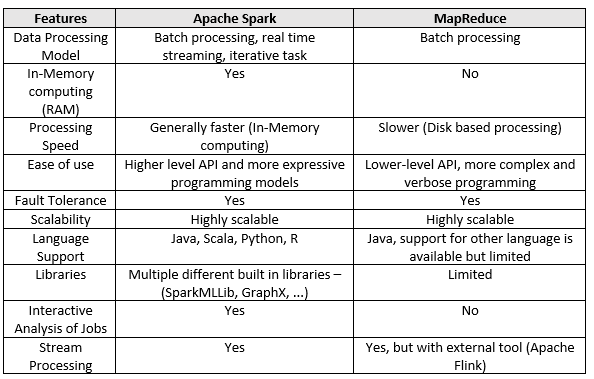
\includegraphics[width=0.99\linewidth]{SparkPaperFigure/SparkVsMapReduce.png}
    \caption{Comparison between Spark and MapReduce}
    \label{fig:SparkVMR}
\end{figure}



%-////////////////////////////////////////////////////////////////////
% \section{Material and Methods}
\subsection{Dataset}
\subsubsection{Cervical Cancer Risk Classification}
This data set can be accessed on Kaggle\cite{kaggle}. The data set has 858 rows and 36 features. The features included are provided in figure \ref{Feature_list} with "Biopsy" being the designated target class.
 

\begin{figure}
    \centering
    
    \begin{tabular}{|m{5em}|m{5em}|m{5em}|}
        
        \hline
         Age&STDs (number)&STDs: HPV  \\
         \hline
         Number of sexual partners& STDs: condylomatosis &STDs: Number of diagnosis\\
         \hline
         First sexual intercourse& STDs:cervical condylomatosis &STDs: Time since first diagnosis\\
         \hline
         Num of pregnancies& STDs: vaginal condylomatosis &STDs: Time since last diagnosis\\
         \hline
         Smokes& STDs: vulvo-perineal condylomatosis & Dx:Cancer\\
         \hline
         Smokes (years)&STDs: syphilis&Dx:CIN	  \\
         \hline
         Smokes (packs/year)&  STDs: pelvic inflammatory disease&Dx:HPV\\
         \hline
         Hormonal Contraceptives& STDs: genital herpes &Dx \\
         \hline
         Hormonal Contraceptives (years)&  STDs: molluscum contagiosum & Hinselmann\\
         \hline
         IUD&  STDs: AIDS & Schiller\\
         \hline
         IUD (years)& STDs: HIV& Citology \\
         \hline
         STDs&  STDs: Hepatitis B & total\_std\\
         \hline
         total\_tests&Biopsy& \\
         \hline
    \end{tabular}
    \caption{All features in Cervical Cancer Risk Classification dataset}
    \label{Feature_list}
\end{figure}		







\subsubsection{Sipakmed}
%Sipakmed, introduced in 2018, is one of the first publicly available dataset for labeled Pap smear images. Sipakmed was developed to standardized and increase availablity for Pap smear images. The dataset consists of 5 different classed, annoted based on the cells cytomorphological fetures.

Sipakmed, introduced in 2018, is one of the first publicly available datasets for labeled Pap smear images\cite{Sipakmed}. Its development aimed to standardize and increase the availability of Pap smear images. The data set encompasses five distinct classes, annotated based on the cytomorphological characteristics of the cells as follows:

\begin{itemize}
    \item Normal Cells
        \begin{itemize}
            \item Superficial-Intermediate Cells
            \item Parabasal Cells
        \end{itemize}
    \item Abnormal Cells
    \begin{itemize}
        \item Koilocytotic Cells
        \item Dyskeratotic Cells
    \end{itemize}
    \item Begnign Cells
    \begin{itemize}
        \item Metaplastic Cells
    \end{itemize}
\end{itemize}

Sipakmed has 966 images, including 4049 cells in total. The specific distribution is shown in Figure \ref{SipakDist}. For the purpose of this project, only the photo of each individual cell is considered for training and testing purposes.

%-////////////////////////////////////////////////////////////////////
\begin{figure}[t]
\vspace{0.5em} % added for space adjustment. Modify/delete for your paper
    \centering
    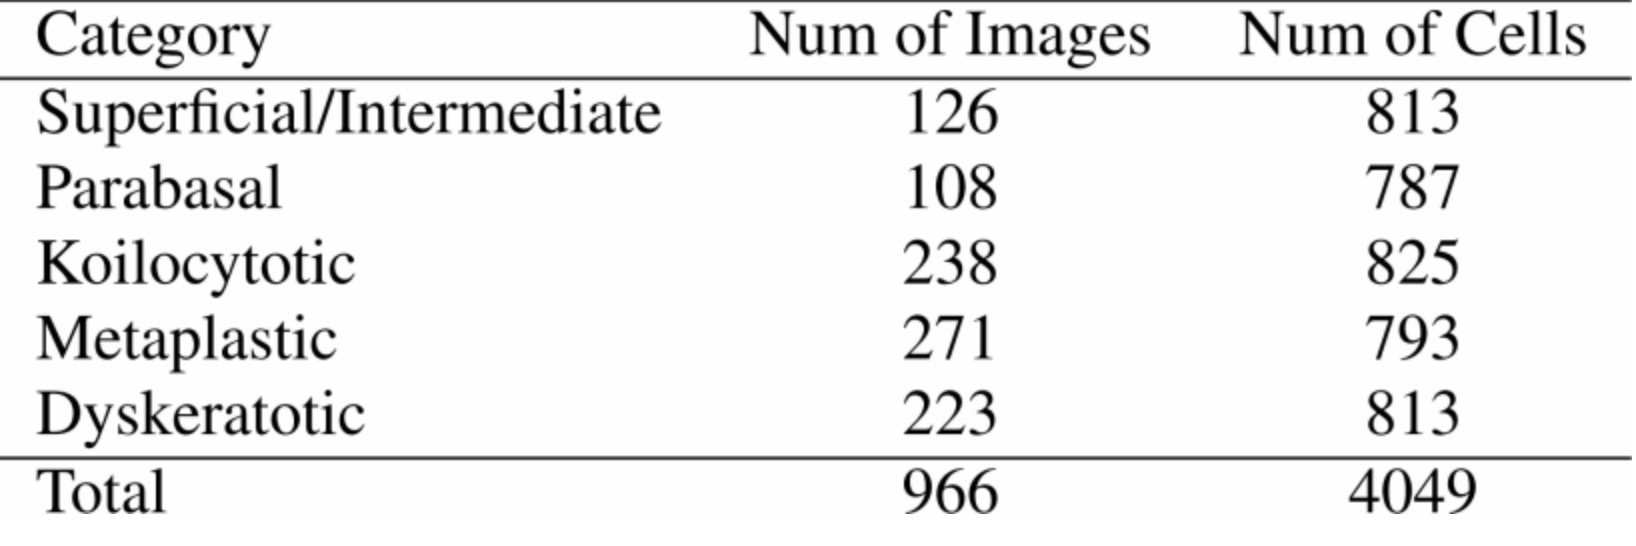
\includegraphics[width=1.0\linewidth]{SparkPaperFigure/Distribution.jpg}
    \caption{Sipakmed's Distribution}
    \vspace{-0.75em} % added for space adjustment. Modify/delete for your paper
    \label{SipakDist}
\end{figure}

\subsection{PreProcessing}
\subsubsection{Cervical Cancer Risk Classfication}
Before the training, several basic steps were taken to make sure the data were ready for machine learning models. First, all "?" values are replaced with the median of their respective columns. Additionally, all duplicated data was removed, resulting in a reduction in the number of rows from 858 to 835 rows.\\
\indent The data set was heavily skewed. Specifically, most of the data set was within the age group of 21 to 32 (Figure \ref{AgeDist}). Other features are also skewed. However, no modification was done to ensure balance on the data set apart from using ADASYN (a super sampling technique) on the "Biopsy" target class. This was necessary due to the imbalanced ratio of 781 to 54 between the values of 0 and 1 for the class of 'biopsy', as demonstrated in Figure \ref{imba-target}.

%-////////////////////////////////////////////////////////////////////
\begin{figure}[t]
\vspace{0.5em} % added for space adjustment. Modify/delete for your paper
    \centering    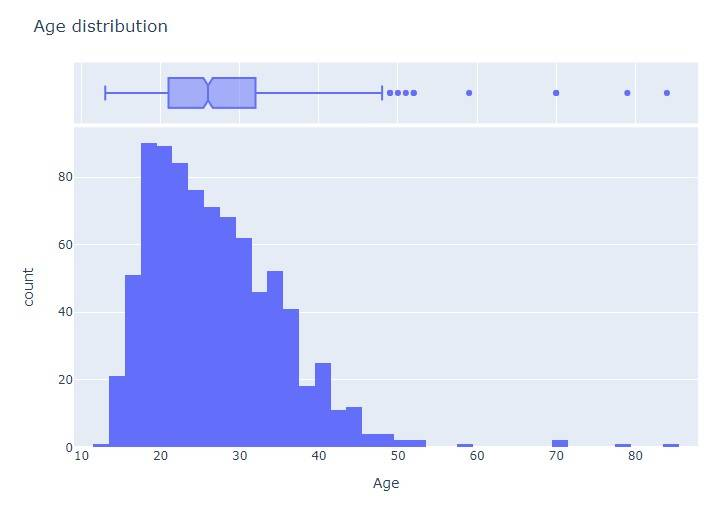
\includegraphics[width=1.0\linewidth]{SparkPaperFigure/Age-Dist.jpg}
    \caption{Age distribution}
    \vspace{-0.75em} % added for space adjustment. Modify/delete for your paper
    \label{AgeDist}
\end{figure}
%-////////////////////////////////////////////////////////////////////

%-////////////////////////////////////////////////////////////////////
\begin{figure}[t]
\vspace{0.5em} % added for space adjustment. Modify/delete for your paper
    \centering

    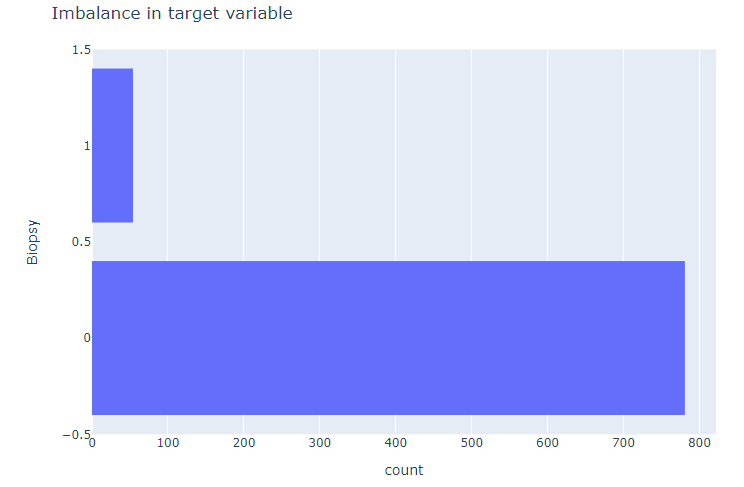
\includegraphics[width=0.9\linewidth]{SparkPaperFigure/imbalance-target-var.png}
    \caption{Imbalance of target variable}
    \vspace{-0.75em} % added for space adjustment. Modify/delete for your paper
    \label{imba-target}
\end{figure}
%-////////////////////////////////////////////////////////////////////

\subsubsection{Sipakmed}
%For Sipakmed data set, first the image is first turn into grayscale, then the images would be compressed to lessen computational burden. Then the compressed image would be convert to dataframe where each features is the color value of that particular pixel. Then standard scaler is applied to the dataframe.

%Since images has lots of pixels, PCA was done to project the dataset to lower dimesionality. All of the process above is doned using SkLearn the reason for which would be explained later. The result after PCA is being saved as CSV and feed to Spark for training and testing.
For the Sipakmed dataset, the initial step involves compressing the images to alleviate the computational load. In this process, the images are resized to a squared dimension of 77x77 pixels. Although it is common to convert images to grayscale to further mitigate computational demands, it was found that grayscale conversion resulted in a 20\% decrease in accuracy during testing. As a result, the decision was made to retain the images' original RGB values without converting to grayscale. Subsequently, the compressed images are transformed into a dataframe structure, where each feature corresponds to the color value of a specific pixel.\\
\indent Given the considerable number of pixels present in the images, Principal Component Analysis (PCA) is conducted to project the dataset into a lower-dimensional space. SkLearn is employed for these pre-processing stages, a choice that will be rationalized in a subsequent explanation. Following PCA, the resulting dataset is saved as a CSV file and input into Apache Spark for subsequent training and testing phases.
\subsection{PCA}
Principal Component Analysis (PCA) is a fundamental technique used to reduce the dimensionality of a dataset while retaining crucial information. In the context of this paper, PCA serves as a vital tool for dimensionality reduction in pap smear cell images. Given an image dataset $X$ comprising $n$ samples, where each sample $x_i$ represents a vector in a high-dimensional space, PCA aims to identify a set of orthogonal vectors (principal components) that capture the maximum variance present in the data. \\
\indent 
Mathematically, the PCA process involves calculating the covariance matrix\cite{mishra2017multivariate}
\begin{equation}
    Sigma = (1/n) * X^T * X, 
\end{equation}
followed by determining its eigenvectors and eigenvalues. Subsequently, the eigenvectors are ordered according to their associated eigenvalues, signifying the directions of maximum variance within the dataset. Through projection onto these principal components, an alternative, lower-dimensional representation of the original data is generated, which effectively retains the predominant variability encapsulated within the dataset. By integrating PCA into our methodology, we can effectively transform patterns inherent in pap smear cell images into a more manageable and informative feature space, thereby facilitating subsequent machine learning tasks.\\
\indent In this case, the images dataframe after compression has dimensions of $4049$ by $17787$. This indicates that the dataframe represents $4049$ photos, each with $17787$ features. The result from PCA analysis demonstrates that $1000$ features are sufficient to explain more than $99\%$ of the original dataframe variance (see Figure \ref{PCA_var}). This substantial reduction in the number of features significantly alleviates the computational overhead required for the classification task.

%-////////////////////////////////////////////////////////////////////
\begin{figure}[t]
\vspace{0.5em} % added for space adjustment. Modify/delete for your paper
    \centering

    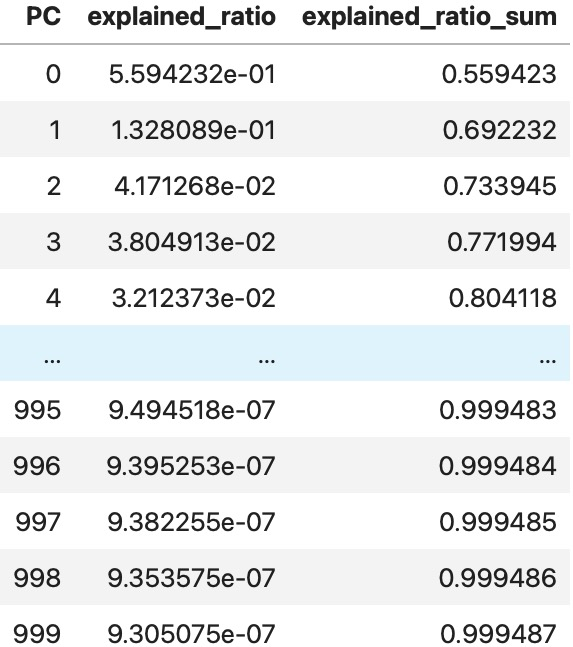
\includegraphics[width=0.5\linewidth]{SparkPaperFigure/PCA_variance.jpg}
    \caption{PCA explained variance}
    \vspace{-0.75em} % added for space adjustment. Modify/delete for your paper
    \label{PCA_var}
\end{figure}
%-////////////////////////////////////////////////////////////////////

\subsection{Model chosen}
\subsubsection{Logistic Regression}
Logistic regression is a linear classification algorithm that models the relationship between input variables and a binary output using the logistic function. It is widely used due to its simplicity and interpretability. Logistic Regression performs well when the relationship between features and the target class is linear. It is computationally efficient and works well with large datasets. However, Logistic Regression may struggle with complex relationships and non-linear data. It assumes linearity and may not capture intricate interactions between variables.
\subsubsection{Decision Tree}
Decision Tree Classifier is a non-parametric algorithm that builds a tree-like model of decisions and their possible consequences. It is intuitive and easy to understand. Decision trees can handle both numerical and categorical data, require minimal data preprocessing, and can capture complex interactions between variables. However, decision trees tend to be prone to overfitting, especially with deep trees. They can be sensitive to small changes in the data, and their interpretability decreases as the tree grows larger.

\subsubsection{Random Forest}
Random Forest Classifier is an ensemble method that combines multiple decision trees to reduce overfitting and improve generalization. It constructs an ensemble of decision trees, where each tree is trained on a random subset of the data and a random subset of the features. Random Forest can handle large datasets, high-dimensional data, and capture complex relationships between variables. However, Random Forest models can be challenging to interpret compared to single decision trees. Training time and memory requirements may increase with a large number of trees in the forest.
\subsubsection{Gradient Boosted Classifier}
Gradient Boosted Classifier is an ensemble method that sequentially builds models, each improving upon the mistakes of the previous ones. It combines weak learners, typically decision trees, in a stage-wise manner. Gradient Boosting can handle complex relationships, works well with heterogeneous data, and can capture feature interactions. It is especially effective in dealing with imbalanced datasets. However, Gradient Boosting can be computationally expensive and may require careful tuning of hyperparameters. It may also be prone to overfitting if the number of boosting iterations is too high.

\subsubsection{Linear Support Vector Machine}
Linear Support Vector Machine (SVM) is a popular classification algorithm that finds the hyperplane that maximally separates the classes in the feature space. SVMs are effective in high-dimensional spaces and can handle both linear and non-linear data by using different kernel functions. They provide robustness against outliers and perform well with small to medium-sized datasets. However, SVMs can be computationally expensive for large datasets and require proper scaling of features. The choice of the kernel function and regularization parameter can significantly impact the performance of SVMs.

\subsubsection{Naives Bayes}
Naive Bayes is a probabilistic classification algorithm that applies Bayes' theorem with the "naive" assumption of feature independence. It is simple, fast, and performs well with high-dimensional datasets. Naive Bayes can handle categorical features and works well with small training sets. It is robust to irrelevant features. However, Naive Bayes assumes feature independence, which may not hold true in real-world scenarios. It may struggle with capturing complex relationships and interactions between variables.

\subsubsection{Factorization Machine Classifier}
Factorization Machine Classifier is a versatile algorithm that models feature interactions in a flexible and scalable manner. It captures complex interactions between features and can handle high-dimensional and sparse data. Factorization Machines are robust to overfitting and require less memory compared to other models. They work well with large-scale datasets and have been successful in various applications, including recommendation systems, click-through rate prediction, and text classification.
\subsection{Experimental Setup and Analysis}
The project has two specific goals: 
\begin{itemize}
    \item \textbf{Demonstrating Spark's Viability as an Alternative Platform}: One of the key aims is to establish Spark as a compelling alternative platform in comparison to traditional machine learning frameworks such as SKLearn or CNN.
    \item \textbf{Comparing Spark's Scalability}: Additionally, the project strives to conduct a  comparison of Spark's scalability in contrast to other non-parallelized platforms, with a particular focus on SKLearn.
\end{itemize}

To address the first objective, the preprocessed data undergoes shuffling and is then divided into a 70-30 training-testing split. Subsequently, the training data is fed into each of the aforementioned machine learning algorithms. This process is repeated ten times, and the resulting outcomes are averaged over these iterations. The default implementation of each algorithm provided by Spark is employed. The methodology is also replicated for the Sipakmed dataset. To evaluate the model performance, a range of performance metrics including accuracy, precision, F1 score, and recall are computed. These results are subsequently compared with those from SkLearn (for CSV files) and CNN (for images) to provide an overview that supports the claim of Spark's viability as a platform.\\
\indent In relation to the second objective, given the challenges encountered during image classification in Spark, the assessment of scalability focuses exclusively on the Cervical Cancer Risk Classification dataset. The initial step involves recording the training time for each machine learning algorithm. Subsequently, the algorithm with the longest training time is selected for further analysis. This chosen algorithm is implemented both in SkLearn and Spark. The chosen algorithm is then applied to a CSV file, which is subsequently duplicated in size with each iteration of the loop. Starting at an initial file size of 268KB, the file grows to a substantial 217MB following ten iterations. Within this context, the singular evaluation metric considered is training time, given that the duplicated data points introduce an element of artificiality. These methodological steps collectively contribute to an exhaustive assessment of Spark's potential as a scalable and viable alternative platform for the context of cervical cancer prediction.\\

\section{Results and Discussion}
\subsection{Accuracy}
\subsubsection{Cervical Cancer Risk Classification}


%-////////////////////////////////////////////////////////////////////
% \begin{figure}[t]
%     \centering

%     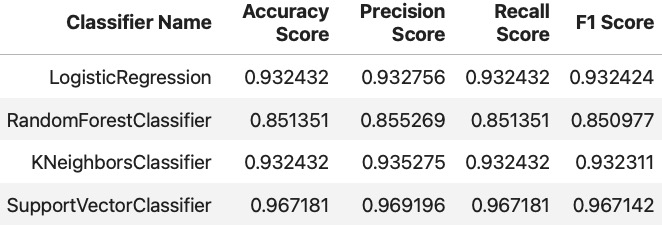
\includegraphics[width=0.9\linewidth]{SparkPaperFigure/SkResult.jpg}
%     \caption{SkLearn's Accuracy on Cervical Cancer Risk Classification }
%     \vspace{-0.75em} % added for space adjustment. Modify/delete for your paper
%     \label{SkChart}
% \end{figure}
%-////////////////////////////////////////////////////////////////////

%-////////////////////////////////////////////////////////////////////
% \begin{figure}[t]
%     \centering

%     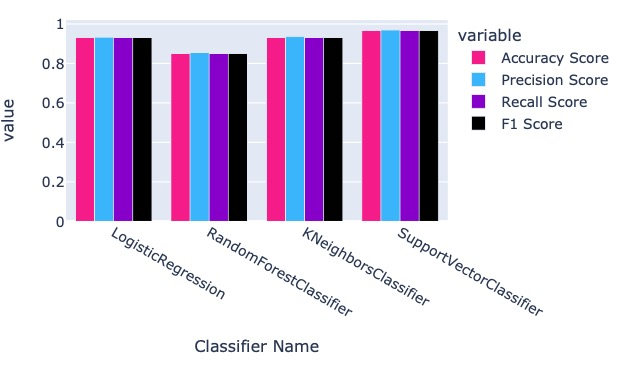
\includegraphics[width=0.9\linewidth]{SparkPaperFigure/SkResultAcc.jpg}
%     \caption{SkLearn's Accuracy on Cervical Cancer Risk Classification}
%     \label{SkTable}
% \end{figure}
%-////////////////////////////////////////////////////////////////////

%%%%%%%%%%%%%%%%%%%%%
%this table about fig 7&8 earlier ones
\begin{table}
    \caption{SkLearn's Accuracy on Cervical Cancer Risk Classification}
    \label{tab:SkLearn's Accuracy on Cervical Cancer Risk}
    
    \begin{center}
    \begin{tabular}{|c|c|c|c|c|}
    \hline
    \textbf{Name} & \textbf{Accuracy} & \textbf{Precision} & \textbf{Recall} & \textbf{F1} \\ \hline
    Logistic Regression  & 0.93 & 0.93 & 0.93 & 0.93 \\ \hline
    Random Forest & 0.85 & 0.86 & 0.85 & 0.85 \\ \hline
    K Nearest Neighbour & 0.93 & 0.94 & 0.93 & 0.93 \\ \hline
    Support Vector Classifier & 0.97 & 0.97 & 0.97 & 0.97 \\ \hline
    
    \end{tabular}
    \end{center}
\end{table}

%%%%%%%%%%%%%%%%%%%

%-////////////////////////////////////////////////////////////////////
% \begin{figure}[t]
%     \centering

%     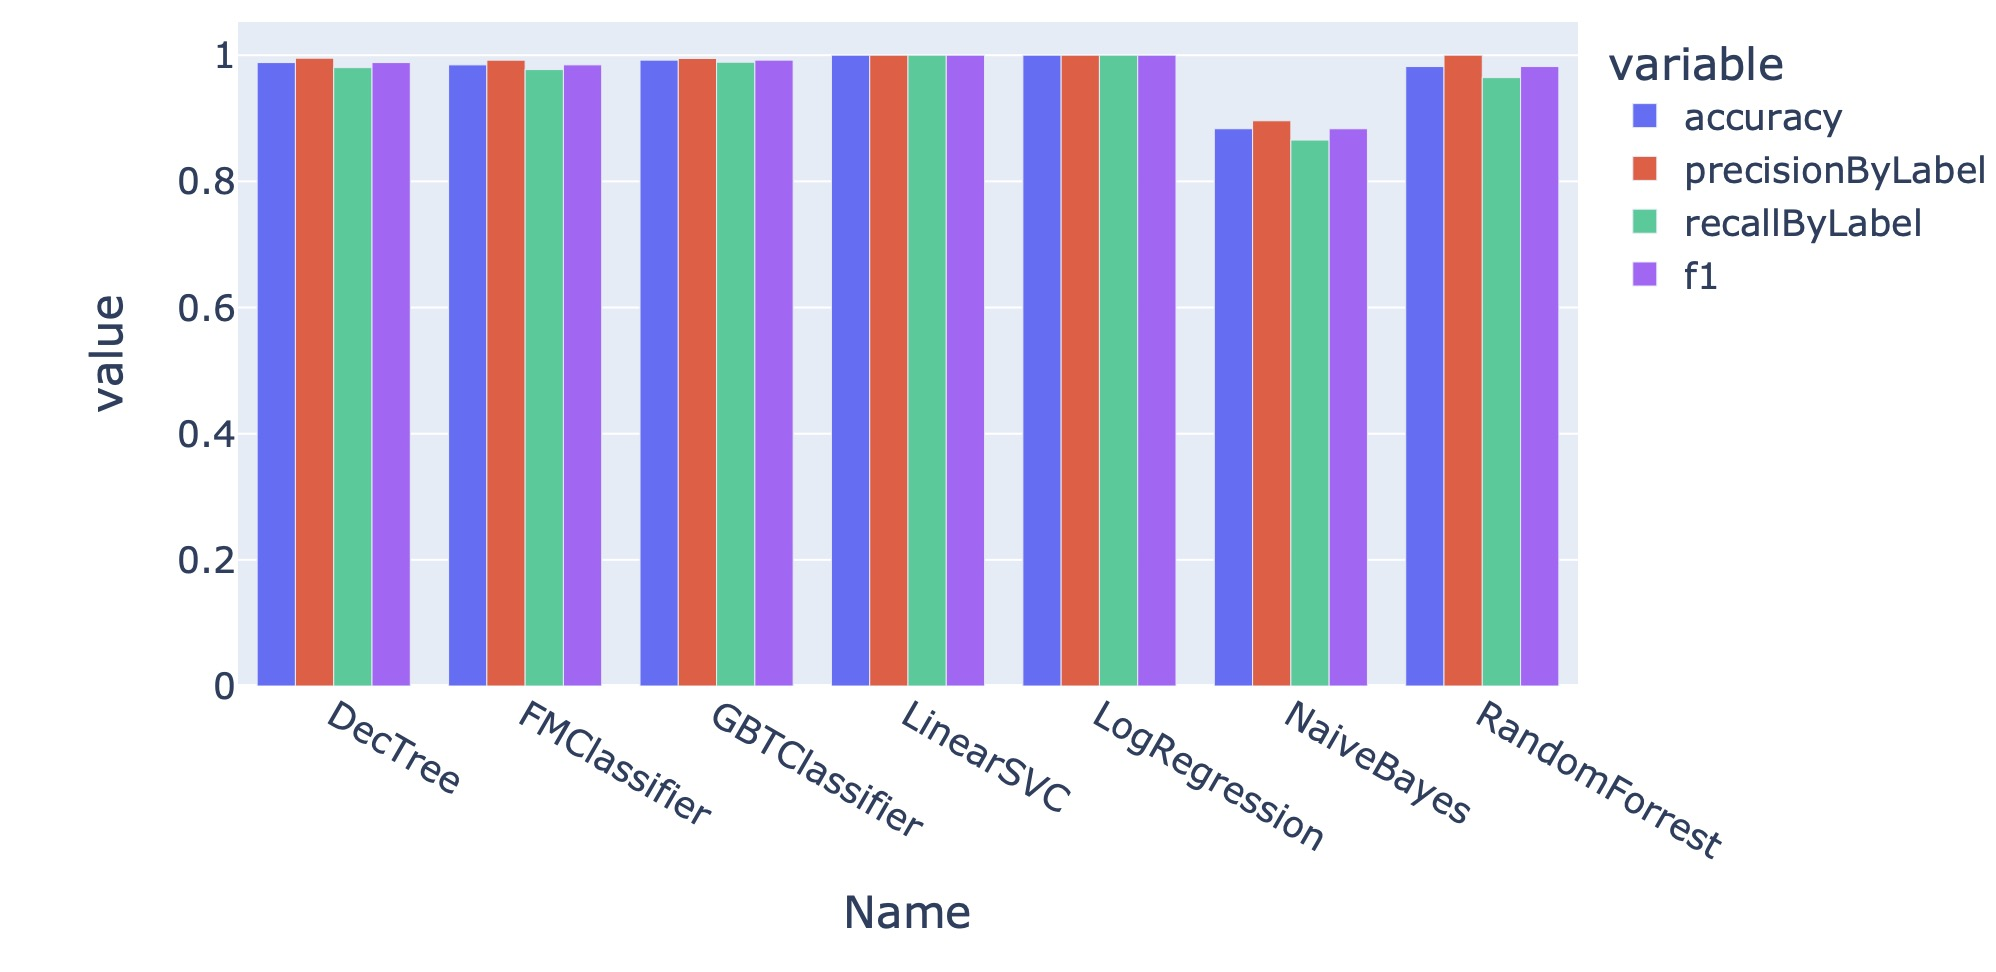
\includegraphics[width=0.9\linewidth]{SparkPaperFigure/Spark-Performance-Og.jpg}
%     \caption{Spark's Accuracy on Cervical Cancer Risk Classification }
%     \vspace{-0.75em} % added for space adjustment. Modify/delete for your paper
%     \label{Spark-Per-OG}
% \end{figure}
%-////////////////////////////////////////////////////////////////////

%-////////////////////////////////////////////////////////////////////
% \begin{figure}[t]
%     \centering

%     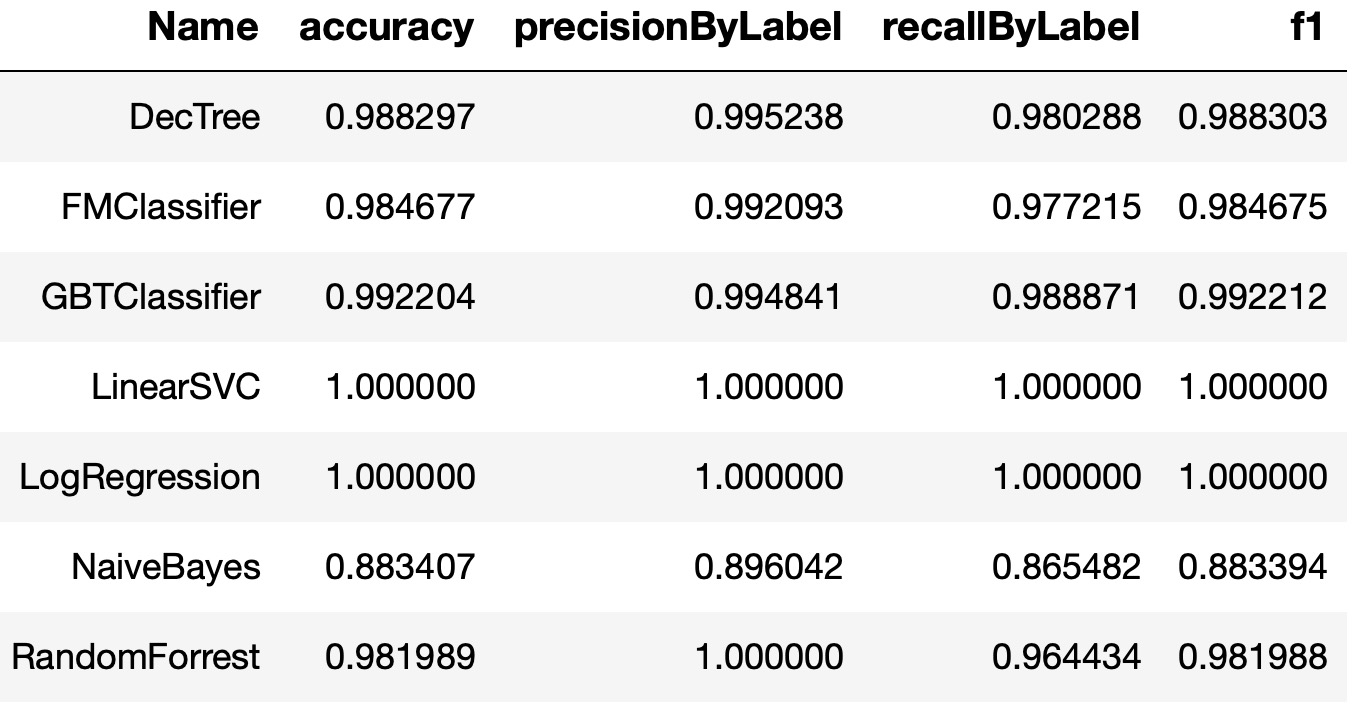
\includegraphics[width=0.9\linewidth]{SparkPaperFigure/acc_chart.jpg}
%     \caption{Spark's Accuracy on Cervical Cancer Risk Classification}
%     \label{Spark-Per-OG-Tab}
% \end{figure}
%-////////////////////////////////////////////////////////////////////

%%%%%%%%%%%%%%%%
\begin{table}
    \caption{Spark's Accuracy on Cervical Cancer Risk Classification}
    \label{tab:model-performance-Spark's Accuracy on Cervical Cancer}
    
    \begin{center}
    \begin{tabular}{|c|c|c|c|c|}
    \hline
    \textbf{Name} & \textbf{Accuracy} & \textbf{Precision} & \textbf{Recall} & \textbf{F1} \\ \hline
    Decision Tree & 0.93 & 0.98 & 0.94 & 0.94 \\ \hline
    FM Classifier & 0.89 & 0.97 & 0.92 & 0.91 \\ \hline
    GBT Classifier & 0.94 & 0.97 & 0.97 & 0.94 \\ \hline
    Linear SVC & 0.95 & 0.99& 0.96 & 0.96 \\ \hline
    Logistic Regression  & 0.93 & 0.98 & 0.95 & 0.94 \\ \hline
    Naive Bayes & 0.82 & 0.98 & 0.83 & 0.86 \\ \hline
    Random Forest & 0.96 & 0.99 & 0.97 & 0.96 \\ \hline
    
    \end{tabular}
    \end{center}
\end{table}


%%%%%%%%%%%%%%%

%Figure \ref{Spark-Per-OG} and Figure \ref{Spark-Per-OG-Tab} show that all  Spark's implemented algorithms are performing well. Notably, all algorithms apart from Naive Bayes exhibit excellent performance, with none falling below 98\% accuracy in any metric.  The Naive Bayes algorithm performs the worst out of all the chosen algorithms. Nevertheless, it still achieves a respectable accuracy of 88\%, while maintaining consistent precision, recall, and F1 scores also around 88\%.

%Figure \ref{SkChart} and figure \ref{SkTable} show the result of the accuracy when implementatd by SkLearn. While the result is lower compared to Spark's implementation, SkLearn's implementation of the code also performs well, with the best result came from Support Vector Classifer which achived score greater than 96\% for all metric. Random forest perform the worst with score around 85\% accross all metrics.

%The result shows that Spark's accuracy is reliable and compared to SkLearn's. However, the exceptional performance of the remaining algorithms raises a valid concern regarding potential overfitting. It is essential to thoroughly investigate this possibility, considering the choices made during the preprocessing stage and the utilization of ADASYN for data balancing. A comprehensive analysis should be conducted to ensure the reliability and generalizability of the models.

%Assuming the absence of major issues in the code implementation, the decision tree algorithm emerges as a promising choice for the given problem. As depicted in Figure \ref{Spark-Time-OG}, this algorithm exhibits an average training time of 0.997 seconds, ranking second in terms of efficiency. Remarkably, despite its efficient performance, the decision tree algorithm maintains consistently high performance levels (above 98\%) across all other metrics, further solidifying its suitability for the task at hand.


% Figures \ref{Spark-Per-OG} and \ref{Spark-Per-OG-Tab}.
As illustrated in Table \ref{tab:model-performance-Spark's Accuracy on Cervical Cancer}, the Spark-implemented algorithms demonstrate robust performance. Notably, except for Naive Bayes, all other algorithms exhibit strong performance, consistently maintaining accuracy rates above 90% for all metrics (the FM classifier also achieves a commendable accuracy of 89%). Despite Naive Bayes performing relatively poorer compared to the other selected algorithms, it still achieves a respectable accuracy of 82%, coupled with a high precision of 99%, albeit with a lower recall of 83%.

% Figures \ref{SkChart} and \ref{SkTable}.
In Table \ref{tab:SkLearn's Accuracy on Cervical Cancer Risk}, the accuracy results when implemented using Scikit-learn are illustrated. While the accuracy rates exhibit a comparable range to those observed in Spark's implementation, the Support Vector Classifier stands out with the best results, achieving accuracy scores exceeding 96\% for all metrics. However, Random Forest performs comparatively less favorably, with accuracy scores hovering around 85\% across all metrics.

For Spark's Implementation, the Random Forest algorithm emerges as a promising solution for the given problem. This is an interesting observation, as the Scikit-learn implementation of the same algorithm yields a much lower result. The difference most likely comes from default parameters of each platform, as we used the default parameters for both platforms. As shown in Figure \ref{Spark-Time-OG}, this algorithm boasts an average training time of 1.18 seconds, ranking as the third most efficient. Remarkably, despite its efficient training, the Random Forest algorithm maintains consistently high performance levels (above 96\%) across all other metrics, further affirming its suitability for the task at hand.


\subsubsection{Sipakmed Dataset}
%Figure \ref{Img_acc},\ref{Img_time} and \ref{Img_table} show the result of for the SipakMed dataset. Overall, the result is not good as no model is able to get to more than 80\% for any metrics.  The best result comes from Decision Tree classifier which achieve higher than 72\% for all metrics. Random forest performs the worst with recall score of 57\%, other metrics achieved above 65\%. While this perfomance is much better than blind guessing since classification is done between 5 classes, this result is far from desireable.

%Figure \ref{CNN_chart} shows that CNN performance is significantly bettern than this paper's Spark implementation. Although program with 32 epochs in mind, by epochs 10, CNN implementation outperform all Spark's implemented algorithm. By epochs 32, CNN achieved accuracy of 92.75\% on the same image set.

%This result show that Spark's or this specific implemenation of Spark is not as suited for image classification task. However, this behaviour is expected as CNN have demonstrated exellent perfomance as images classification task.\cite{CNN}

% \ref{Img_time}, and \ref{Img_table} 
In Table. \ref{tab:spark-accuracy-sipakmed}, the results for the SipakMed dataset regarding Spark accuracy are presented. Overall, the outcomes are suboptimal, with no model surpassing the 80\% mark for any metrics. The most favorable performance is observed in the Decision Tree classifier, achieving scores above 72\% for all metrics. On the other end of the spectrum, Random Forest performs the least effectively, with a recall score of 57\%, although other metrics achieve scores above 65\%. While this performance surpasses random guessing, considering the classification task's complexity across five classes, the results remain far from desirable.

Historically, Convolutional Neural Networks (CNNs) have excelled in image classification tasks\cite{CNN}. Figure \ref{fig-CNN_chart} showcases the significant superiority of CNN performance compared to the Spark implementation in this paper as in Figure \ref{Img_time}. Despite being designed with 32 epochs in mind, CNN outperforms all of Spark's implemented algorithms as early as epoch 10. By the 32nd epoch, CNN attains an accuracy of 92.75\% on the same image dataset.

 This result highlights the fact that image classification is not an area where Spark demonstrates strength, especially in comparison to specialized deep learning frameworks like TensorFlow or PyTorch that leverage GPU acceleration. While Spark ML serves as a versatile tool for distributed computing tasks, its architecture and default configurations are not optimized for the intricacies of image processing and deep learning. 

%-////////////////////////////////////////////////////////////////////
\begin{figure}[t]
\vspace{0.5em} % added for space adjustment. Modify/delete for your paper
    \centering

    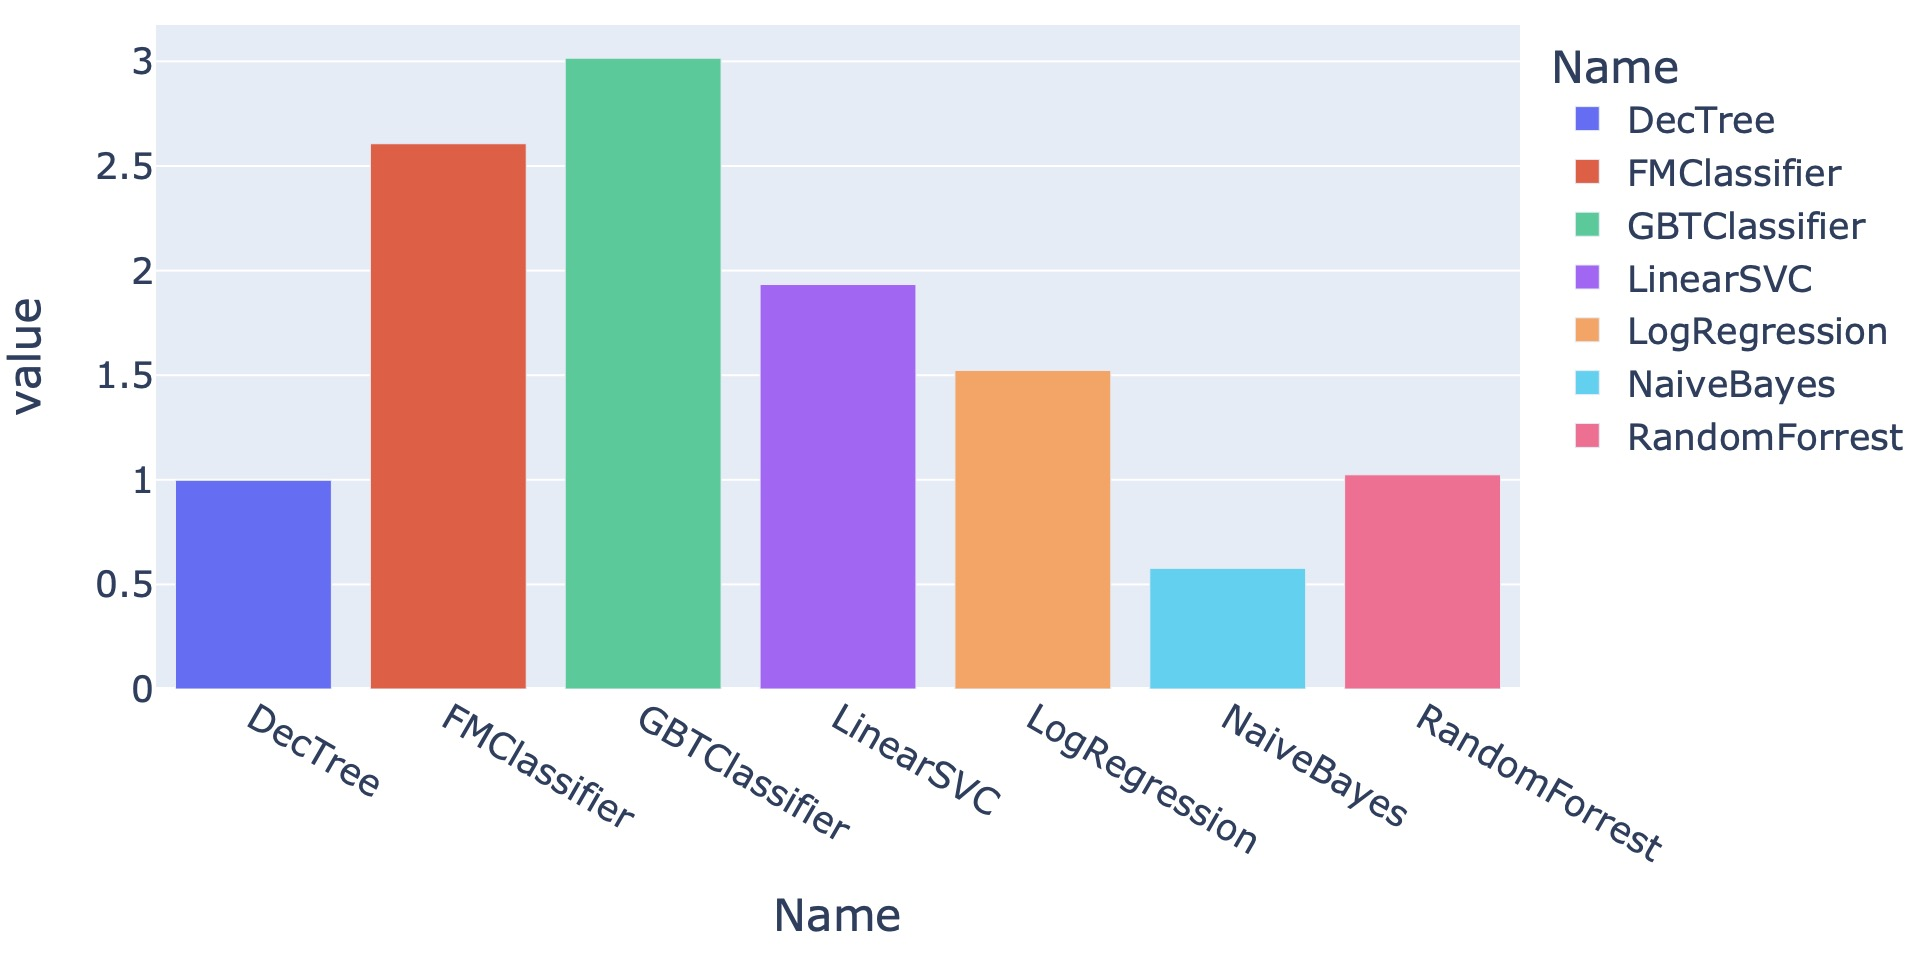
\includegraphics[width=0.9\linewidth]{SparkPaperFigure/Spark-Time-Og.jpg}
    \caption{Spark's Training Time (Cerivical Cancer Classification)}
    \label{Spark-Time-OG}
\end{figure}
%-////////////////////////////////////////////////////////////////////
\begin{figure}[t]
\vspace{0.5em} % added for space adjustment. Modify/delete for your paper
    \centering

    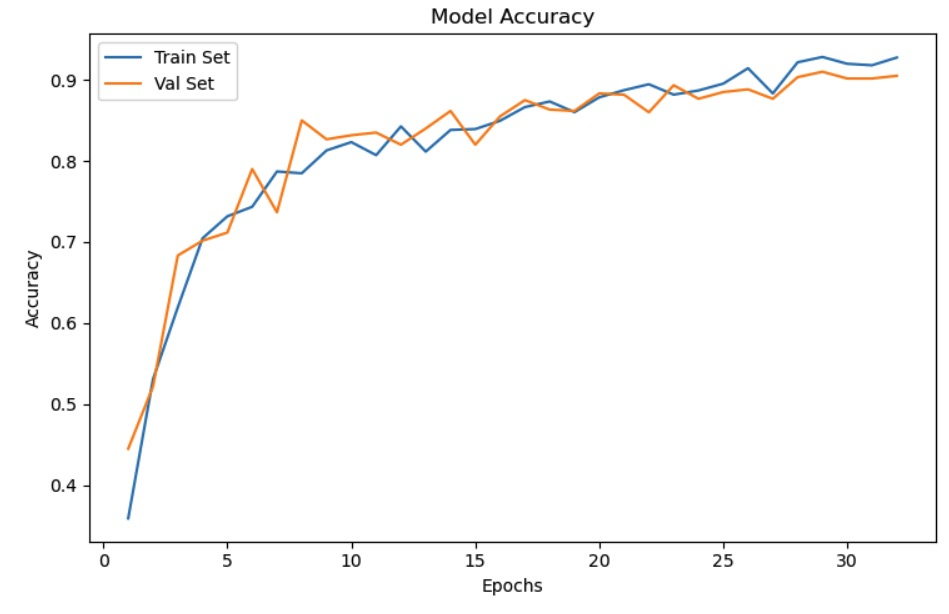
\includegraphics[width=0.9\linewidth]{SparkPaperFigure/CNN.jpg}
    \caption{CNN's Accuracy (SipakMed)}
    \label{fig-CNN_chart}
\end{figure}
%-////////////////////////////////////////////////////////////////////
% \begin{figure}[t]
% \vspace{0.5em} % added for space adjustment. Modify/delete for your paper
%     \centering

%     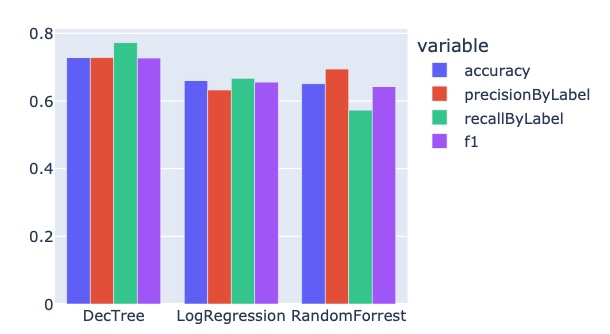
\includegraphics[width=1.05\linewidth]{SparkPaperFigure/Image_acc.jpg}
%     \caption{Spark's Accuracy (SipakMed)}
%     \label{Img_acc}
% \end{figure}
%-////////////////////////////////////////////////////////////////////
%-////////////////////////////////////////////////////////////////////

%-////////////////////////////////////////////////////////////////////
%-////////////////////////////////////////////////////////////////////
% \begin{figure}[t]
% \vspace{0.5em} % added for space adjustment. Modify/delete for your paper
%     \centering

%     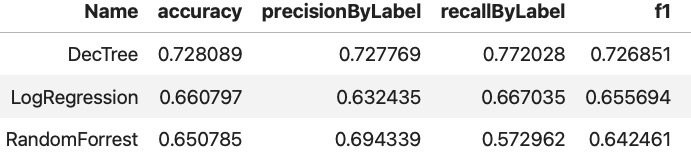
\includegraphics[width=0.9\linewidth]{SparkPaperFigure/ImgTable.jpg}
%     \caption{Spark's Accuracy (SipakMed)}
%     \label{Img_table}
% \end{figure}
%-////////////////////////////////////////////////////////////////////
%%%%%%%%%%%%%%%%%%%%%%
\begin{table}
    \caption{Spark's Accuracy (SipakMed)}
    \label{tab:spark-accuracy-sipakmed}
    
    \begin{center}
    \begin{tabular}{|c|c|c|c|c|}
    \hline
    \textbf{Name} & \textbf{Accuracy} & \textbf{Precision} & \textbf{Recall} & \textbf{F1} \\ \hline
    Decision Tree & 0.73 & 0.73 & 0.77 & 0.73 \\ \hline
    Logistic Regression  & 0.66 & 0.63 & 0.67 & 0.66 \\ \hline
    Random Forest & 0.65 & 0.70 & 0.57 & 0.64 \\ \hline
    
    \end{tabular}
    \end{center}
\end{table}






%%%%%%%%%%%%%%%%%%%%



\subsection{Scalability}
%-////////////////////////////////////////////////////////////////////
\begin{figure}[t]
\vspace{0.5em} % added for space adjustment. Modify/delete for your paper
    \centering

    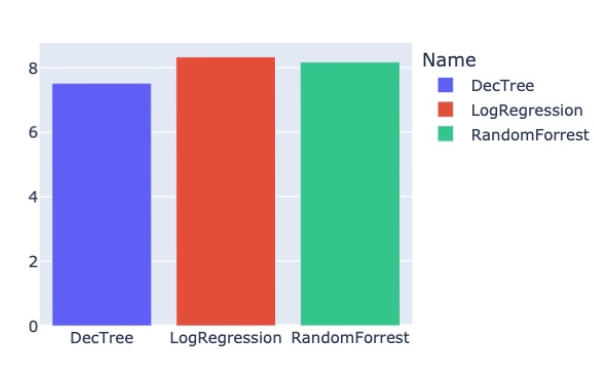
\includegraphics[width=0.9\linewidth]{SparkPaperFigure/ImgTrainingtime.png}
    \caption{Spark's Training time (SipakMed)}
    \label{Img_time}
\end{figure}
%-////////////////////////////////////////////////////////////////////


%-////////////////////////////////////////////////////////////////////
\begin{figure}[t]
\vspace{0.5em} % added for space adjustment. Modify/delete for your paper
    \centering

    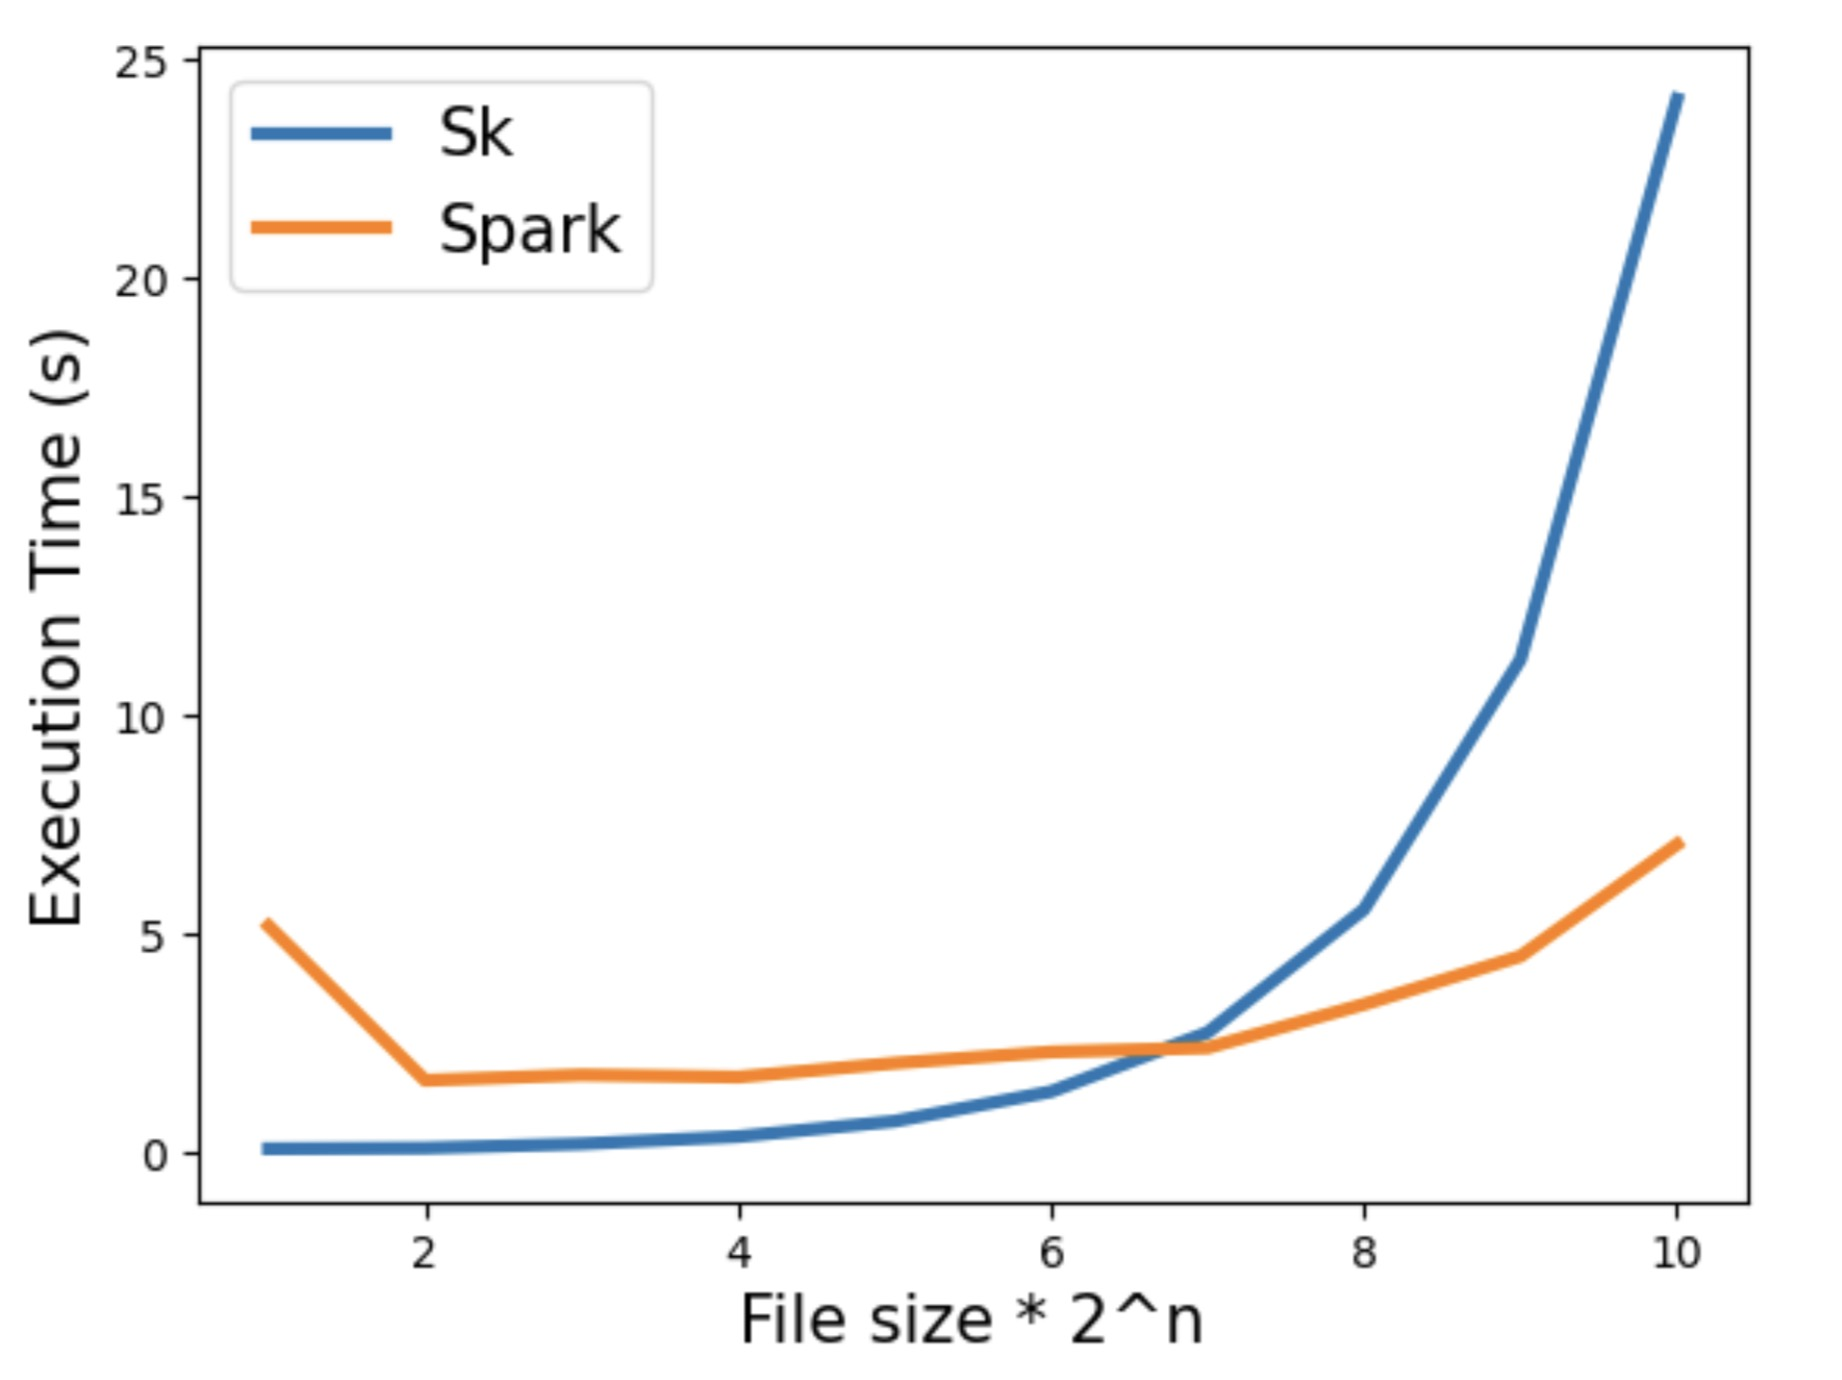
\includegraphics[width=0.9\linewidth]{SparkPaperFigure/Scale-Sk-Spark.jpg}
    \caption{Scalability (Chart)}
    \label{fig-Scale_graph}
\end{figure}
%-////////////////////////////////////////////////////////////////////

%-////////////////////////////////////////////////////////////////////
% \begin{figure}[t]
% \vspace{0.5em} % added for space adjustment. Modify/delete for your paper
%     \centering

%     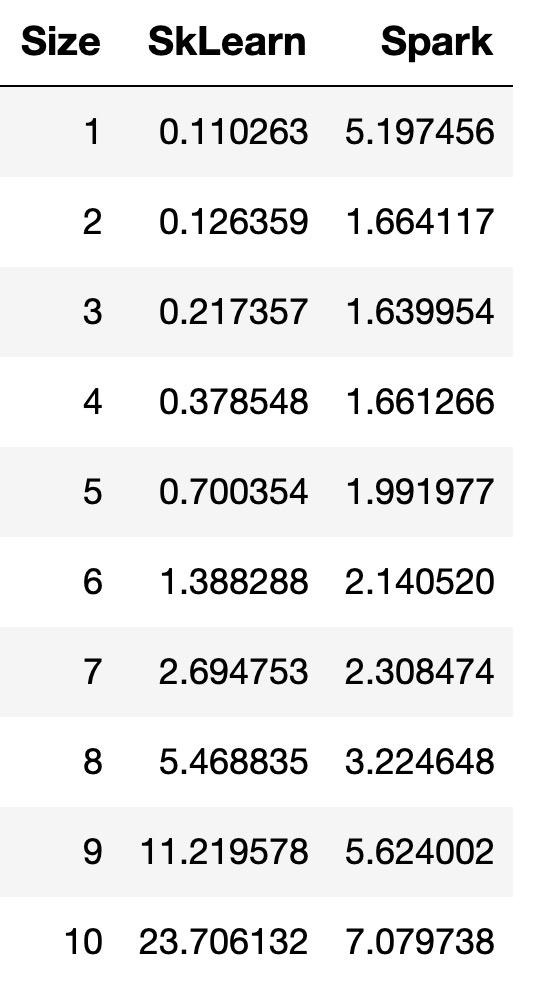
\includegraphics[width=0.9\linewidth]{SparkPaperFigure/Scale_table.jpg}
%     \caption{Scalability (Table)}
%     \label{Scale_table}
% \end{figure}
%-////////////////////////////////////////////////////////////////////


%%%%%%%%%%%%%%
\begin{table}
    \caption{Scability of SKLearn and Spark}
    \label{tab:model-performance-sklearn-spark}
    
    \begin{center}
    \begin{tabular}{|c|c|c|}
    \hline
    \textbf {Size} & \textbf{SkLearn (s)} & \textbf{Spark (s)}   \\ \hline
    1 & 0.110263 & 5.197456  \\ 
    \hline
    2 & 0.126359 & 1.664117  \\ \hline
    3 & 0.217357 & 1.639954  \\ \hline
    4 & 0.378548 & 1.661266  \\ \hline
    5 & 0.700354 & 1.991977  \\ \hline
    6 & 1.388288 & 2.140520  \\ \hline
    7 & 2.694753 & 2.308474  \\ \hline
    8 & 5.468835 & 3.224648  \\ \hline
    9 & 11.219578 & 5.624002  \\ \hline
    10 & 23.706132 & 7.079738  \\ \hline
    
    \end{tabular}
    \end{center}
\end{table}


%%%%%%%%%%%

Figure \ref{Spark-Time-OG} illustrates the training times of various algorithms, guiding the selection of the Gradient Boosted Tree algorithm for scalability testing due to its longer training duration.

As shown in the Fig. \ref{fig-Scale_graph}, SkLearn's fitting time doubles with each iteration, reflecting its lack of parallelization. This behavior aligns with expectations, considering the proportional increase in training time with growing file size. In contrast, Spark exhibits a distinct pattern. While the initial iteration involves additional setup time for parallelization, subsequent iterations demonstrate a significant performance advantage over SkLearn. Notably, Spark maintains consistent and comparatively faster training times from the second to the fourth iteration, hovering around 1.6 seconds.

As shown in the Table \ref{tab:model-performance-sklearn-spark},
Spark's training time, after the initial setup in the first iteration, remains relatively steady across iterations 2, 3, and 4. Remarkably, starting from the seventh iteration, Spark exhibits a substantial performance improvement, achieving considerably faster training times.\\
\indent While SkLearn showcases a relatively faster training time in percentage terms before the sixth iteration, the practical difference between instant completion and a 2-second interval remains minimal. However, as the iterations progress, Spark's lead becomes evident, resulting in a 16-second difference in training time by the tenth iteration. This means, the scalability of spark grows three times than the SkLearn in the 10th iterations, reducing the time complexity. This emphasizes Spark's superiority in terms of scalability.

These findings show that Spark has significant advantage over SkLearn when managing larger datasets and achieving efficient parallel processing. Spark's capability to deliver consistent and fast performance, even as data size increases, solidifies its position as the preferred platform for scalable text based machine learning tasks.

\section{Spark's Implementation Issues}

Despite Spark's demonstrated scalability with larger text data and satisfactory performance with smaller datasets, certain issues arise in its implementation:

\begin{itemize}
    \item \textbf{Performance Discrepancies Between Platforms}: In this research scope, significant performance variations were observed between Spark instances running on different hardware setups. For example, Spark exhibited notably faster execution on an M1 chip compared to a Windows machine equipped with an i7-12700 processor. While the training of the smallest model on the Windows machine took at least 50 seconds, the M1 chip completed the same task, including setup time, in just 5.3 seconds.

    \item \textbf{Popularity and Algorithm Availability}: Unlike Scikit-learn, Spark has a smaller user base, resulting in fewer available algorithms. While the SparkML library offers a diverse range of algorithms, it may not provide as extensive a selection as Scikit-learn. Users may find a wider range of readily accessible algorithms within the Scikit-learn ecosystem.
\end{itemize}

Furthermore, while not directly related to Spark as a library, developing custom algorithms within the Spark framework can be significantly more complex compared to Scikit-learn. To fully leverage Spark's capabilities, users need to understand additional concepts such as MapReduce and Resilient Distributed Datasets (RDDs). This steep learning curve may require users to invest more time and effort to extract the maximum benefits from Spark. We encountered this firsthand when attempting image classification tasks, where the traditional workflow involving image compression, grayscale transformation, and subsequent PCA proved challenging. Despite having 32GB of RAM, loading images and applying PCA resulted in memory overflow. Upgrading to a system with 128GB of RAM allowed PCA processing to begin, but after approximately 15 minutes, Spark's PCA implementation unexpectedly reduced the dataset's dimensionality, contrary to PCA's intended function. This issue stemmed from both code implementations and potential limitations in Spark's PCA implementation. However, we addressed this issue by using PCA from Scikit-learn, saving the output as a CSV, and then feeding it into Spark. Nonetheless, the inability to perform all tasks solely within the Spark ecosystem remains a constraint.2

Overall, Spark offers significant scalability benefits and a comprehensive machine learning library suitable for diverse computational environments, including those primarily utilizing CPUs. Nevertheless, it is imperative to acknowledge potential performance discrepancies based on hardware configurations, algorithm availability with respect to SkLearn, and the additional expertise required to effectively wield Spark. Furthermore, Spark may not be as well-suited for certain machine learning tasks, such as image classification, which can benefit from specialized hardware like GPUs."

\section{Conclusion}
Our research has revealed that Spark is a viable option for the medical sector, particularly in the area of cervical cancer prediction. All algorithms tested for CSV file showed excellent results, with most achieving an accuracy of 98\% or higher. Furthermore, Spark was able to efficiently manage large datasets, which is essential given the growing availability of data from IoT devices that can be used to improve machine learning model performance. It is important to note that Spark is not a universal solution for all machine learning problems. There are many difficulties encounter when trying to make image recognition works on Spark. But in the context of big data, the field of machine learning should be moving towards increased parallelization. Spark's capabilities are well-suited to this trend, making it a valuable tool for taking advantage of the potential of big data in medical applications and beyond. A key aspect of the research is its multimodal approach to cervical cancer detection, analyzing structured data in CSV format and unstructured image data. By addressing the detection challenge from multiple angles, the study underscores the potential of Spark in processing various data types for healthcare applications, paving the way for more comprehensive and effective diagnostic solutions.
In future works, we plan to explore about image classification in general settings using Spark implementations for other modalities, that might help in improvements in scalability issues.

\chapter{Patient-Centric Blockchain for EHRs}\label{chap:blockchain}

\noindent\emph{Chapter bridge.} This chapter builds the consent layer that the
federated system depends on, and---just as importantly---the \emph{instrument} for
measuring its cost. It presents a patient-controlled health-record system in which
an Ethereum smart contract holds permissions, content identifiers, and keys while
the clinical payload sits encrypted off-chain on IPFS, exposing grant and revoke
operations whose latency and gas cost are measured on both a local chain and a
public testnet. Those grant/revoke semantics become the patient-consent tier of
the two-tier consent layer in Chapter~\ref{chap:fl_clusters}, and the on-chain
cost-measurement methodology established here is exactly what RQ1
(Section~\ref{sec:thesis}) reuses to quantify governance overhead per federated
round. This chapter is adapted from the candidate's published work~\cite{nhan2024ehr}.

\section{Introduction}

\subsection{EHR and Current Deployment}
Electronic Health Record (EHR) systems are integral to the digitization of healthcare, enabling the storage, retrieval, and management of patient health information electronically. Despite their advantages in improving the efficiency and quality of healthcare services, EHR systems are plagued by challenges such as centralization, which leads to single points of failure and potential system downtimes. Also, since data is centralized, patients have no control over their data, leading to potential abuse. Additionally, the lack of standardization across different EHR systems complicates the interoperability and seamless exchange of patient information across various healthcare providers. Furthermore, these systems often fall short in ensuring robust security measures, leaving sensitive patient data vulnerable to breaches and unauthorized access. These challenges not only compromise patient privacy and trust but also hamper the scalability and adaptability of healthcare services to meet evolving needs. The introduction of blockchain technology promises to address these issues by decentralizing data storage, enhancing data security, and improving interoperability through standardized protocols, paving the way for a more resilient and patient-centric healthcare ecosystem.


% Make sure to keep this image from unncessary floating. Keep this image  between Motivation and Why Blockchain?
\begin{figure}[!b]
    \centering
    \resizebox{\columnwidth}{!}{%
        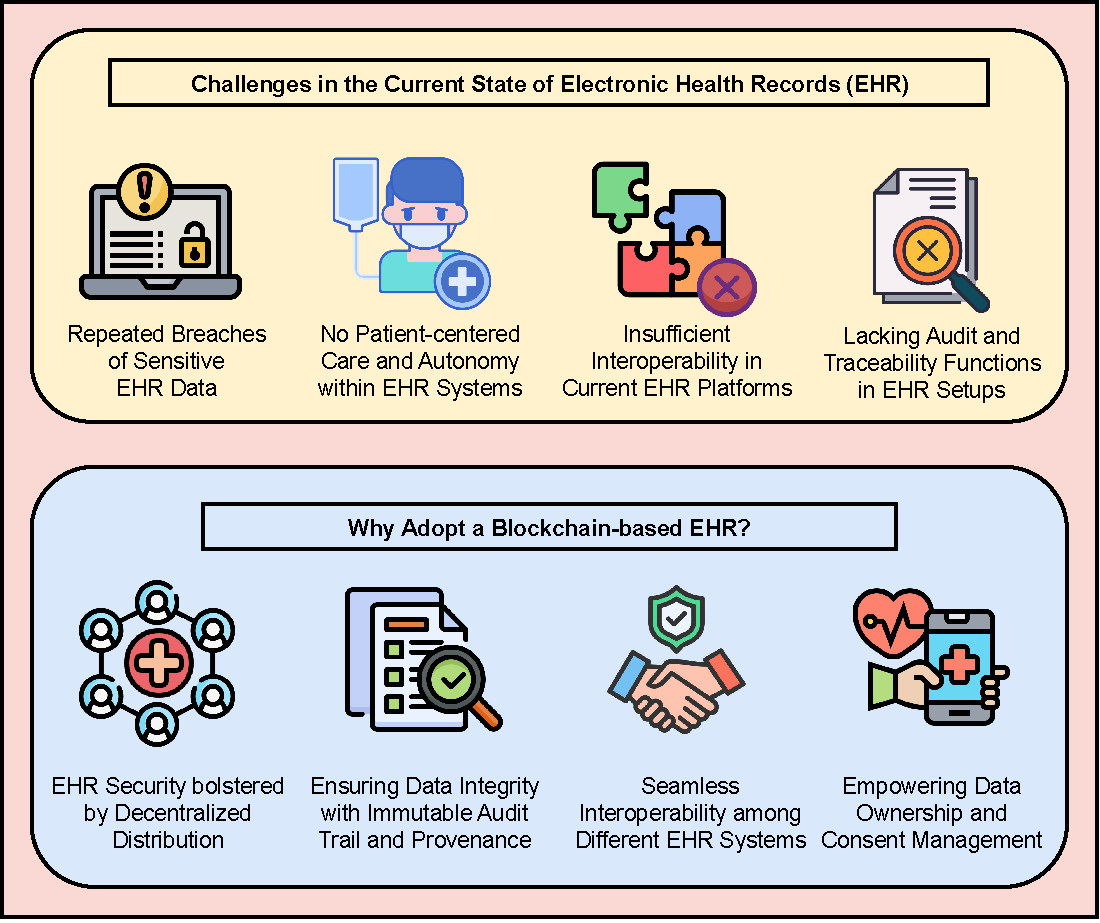
\includegraphics[width=0.3\linewidth]{BlockChainPaper/Problem-Motivation.pdf}
    }
    \caption{The inherent incapability and vulnerability present-day EHR systems causes concerns with breaches, autonomy, and interoperability. This emphasizes how important it is for EHRs to implement blockchain technology, which offers improved security, integrity, interoperability, and patient empowerment in addition to numerous other benefits when handling healthcare data.}
    
    \label{fig:problem-motivation}
\end{figure}

\subsection{Problem Motivation}
The motivation behind this research stems from the want to overcome the limitations of current EHR systems. With healthcare data breaches on the rise and the increasing demand for seamless healthcare data exchange, it is necessary to explore different solutions that can bolster the security, reliability, and efficiency of EHRs.

Expanding on this motivation, we can delve into several key points:

\begin{enumerate}
    \item \textbf{Repeated Breaches of Sensitive EHR Data:} The total NIA (number of individuals affected) is 173,627,498 (roughly 173.6 million people) between Oct 2009 and Jun 2017. On average, one data breach takes place every 1.5 days \cite{koczkodaj2019massive}. Healthcare data breaches pose a significant threat to patient confidentiality and trust in healthcare systems. Recent incidents highlight the vulnerability of centralized data storage, underscoring the need for alternative approaches to data security.
    
    \item \textbf{No Patient-centered Care and Autonomy within EHR Systems:} Empowering patients with greater control over their health information is essential for fostering patient-centered care models. Enhancing data accessibility and transparency not only promotes patient autonomy but also enables informed decision-making and personalized treatment plans.

    \item \textbf{Insufficient Interoperability in Current EHR Platforms:} The lack of interoperability among existing EHR systems hampers the seamless exchange of patient information between healthcare providers. This fragmentation impedes timely access to critical medical data, leading to inefficiencies and potentially compromising patient care.

    \item \textbf{Lacking Audit and Traceability Functions in EHR Setups:} The capabilities of EHR systems today are insufficient for tasks like data tracking and fair audits. This makes it more difficult to keep an eye on and validate data access, usage, and integrity within the system.  
\end{enumerate}




\subsection{Why Blockchain?}

Blockchain technology, showing potential across multiple domains, offers a robust solution to various longstanding challenges by ensuring decentralization, transparency, and security. Its inception, popularized through Bitcoin \cite{nakamoto2008bitcoin}, laid the groundwork for its extensive applicability. In sectors such as electronic voting, music, renewable energy, and e-government, blockchain enhances legitimacy, transparency, and operational efficiency \cite{BlockchainVotingJafar2021, BlockchainMusicChavan2019, BlockchainRenewableEnergyGorski2022, BlockchainEgovernmentWang2022}. Similarly, it promises improvements in smart education, coffee distribution, energy management, image copyright protection, identity management, and legal documentation, by ensuring a secure, decentralized approach to data management and exchange \cite{BlockchainSmartEducationDubey2023, BlockchainCoffeeDistributionInayatulloh2023, BlockchainEnergyManagementWang2023, BlockchainImageCopyrightXiao2023, BlockchainIdentity, BlockchianPoliceRecord}.

In the healthcare domain, blockchain emerges as a robust solution to several challenges in healthcare data management. Its decentralized architecture increases system reliability by removing single points of failure. The immutability of blockchain records strengthens data integrity and trustworthiness, critical for secure health data management. Moreover, blockchain facilitates seamless data exchange across diverse EHR systems through smart contracts and consensus mechanisms, envisioning an EHR system paradigm that is secure, interoperable, and centered around patient care.

Expanding on the rationale for utilizing blockchain technology in healthcare, we explore the following aspects:

\begin{enumerate}
    \item \textbf{EHR Security Bolstered by Decentralized Distribution:} By distributing data across a network of nodes, blockchain eliminates reliance on centralized authorities, reducing the risk of data manipulation or unauthorized access. This decentralized approach enhances system resilience and mitigates the impact of potential security breaches.
    
    \item \textbf{Ensuring Data Integrity with Immutable Audit Trail and Provenance:} The immutable nature of blockchain transactions ensures that once data is recorded, it cannot be altered or tampered with retroactively. This feature provides a transparent audit trail of data interactions, enhancing accountability and facilitating compliance with regulatory requirements.
    
    \item \textbf{Seamless Interoperability among Different EHR Systems:} Blockchain's standardized protocols and interoperable nature enable integration with existing EHR systems and healthcare infrastructure.
    
    \item \textbf{Empowering Data Ownership and Consent Management:} Blockchain-based solutions empower patients to maintain ownership of their health data and control access permissions. Smart contracts can enforce consent mechanisms, allowing patients to specify who can access their data and under what conditions, fostering trust and transparency in healthcare transactions.
\end{enumerate}

\subsection{Our Contributions}
\begin{itemize}
    \item We develop a novel framework for the integration of blockchain technology into electronic health records systems, enhancing data integrity, security, and patient privacy.
    \item We introduce a patient-centric model that empowers individuals with high control and access over their health data, promoting autonomy in personal health data management.
    \item We design and implement robust security protocols that leverage the decentralized nature of blockchain to safeguard against unauthorized data breaches and access, ensuring a secure environment for patient data.
    \item We have implemented a modular system designed to accommodate changes in components if necessary, such as the security method.
\end{itemize}

\subsection{Outline}
This paper is structured to explore the application of blockchain technology in EHR systems. Section 2 delves into the background and existing literature, providing a comprehensive brief  EHR paper with blockchain. Section 3 details the methodology employed in this study, including the design and implementation of our blockchain-based EHR system. Section 4 presents the results of our research, showcasing the practical benefits and challenges encountered during the implementation phase. Section 5 discusses the limitations of our current system and proposes directions for future research. Finally, Section 6 concludes the paper by summarizing our findings, highlighting the potential of blockchain to revolutionize EHR systems, and suggesting areas for further investigation to fully harness the benefits of this technology in healthcare.


\section{Existing Studies }

% \newcommand{\xmark}{\text{\texttimes}} % Duplicate definition removed
\begin{table}[h]
\centering
\resizebox{\columnwidth}{!}{%
\begin{tabular}{lccccccc}
\hline
\textbf{Reference}            & \cite{singh2023exploring} & \cite{azaria2016medrec} & \cite{kuo2017distributedled} & \cite{abdelsalam2023blockchain} & \cite{yue2016healthcare} & \cite{schmeelk2022electronic} & \textbf{Our Work} \\
\hline
\textbf{Year}                 & 2023                       & 2016                    & 2017                         & 2023                             & 2016                     & 2022                            & \textbf{2024}          \\
\textbf{Use of Smart Contract}& \checkmark                & \checkmark              & \checkmark                   & \xmark                        & \xmark                  & \xmark                          & \textbf{\checkmark}     \\
\textbf{Use Blockchain}       & \checkmark                & \checkmark              & \checkmark                   & \checkmark                       & \checkmark              & \checkmark                      & \textbf{\checkmark}     \\
\textbf{Implement EHR System} & \xmark                    & \checkmark              & \checkmark                   & \checkmark                       & \checkmark              & \checkmark                      & \textbf{\checkmark}     \\
\textbf{Load Testing on Live Network} & \xmark           & \xmark                  & \xmark                       & \xmark                           & \xmark                  & \xmark                          & \textbf{\checkmark}     \\
\textbf{Testing on Local Network} & \xmark              & \xmark                  & \xmark                       & \xmark                           & \xmark                  & \xmark                          & \textbf{\checkmark}     \\
\hline
\end{tabular}
}
\caption{Comparison highlighting all main points, including our novel methodological approach to EHR and blockchain, not covered by other papers in this domain.}
\label{table:comparison}
\end{table}


The integration of blockchain technology in healthcare has been a subject of considerable interest in recent years. Studies by Singh et al.~\cite{singh2023exploring} and Abdelsalam~\cite{abdelsalam2023blockchain} have highlighted the promising aspects of blockchain as an alternative to traditional databases for healthcare applications, emphasizing its potential for ensuring data integrity, enhancing security, and improving interoperability within healthcare systems.

Further contributions by Azaria et al.~\cite{azaria2016medrec}, Kuo et al.~\cite{kuo2017distributedled}, and Yue et al.~\cite{yue2016healthcare} have moved beyond the conceptual phase to create real-world models and prototypes that showcase the practical applications of blockchain in managing Electronic Health Records (EHR). These works provide valuable insights into the deployment of blockchain technologies for healthcare data management, though they predominantly focus on the developmental stage, with limited discussion on comprehensive load testing or extensive real-world implementation.

Schmeelk et al.~\cite{schmeelk2022electronic} further explore the interoperability requirements and the use of blockchain for privacy-preserving data analysis in healthcare. However, like the preceding studies, this research also indicates a gap between the theoretical framework and practical application, particularly in the context of load testing and system scalability.

Our work seeks to address these limitations by implementing an EHR system that leverages blockchain technology, enhanced by smart contracts for data management and the InterPlanetary File System (IPFS) for distributed storage. This approach not only aims to validate the theoretical benefits of blockchain in healthcare but also to demonstrate its practical viability and scalability through more load testing on both live and local networks, moving beyond the prototype stage to offer and try to offer a more user-centric model for healthcare data management.

\section{Methodology}
\subsection{Overview of system Architecture}
The architecture of our Electronic Health Records (EHR) system is designed with an emphasis on security, efficiency, and user accessibility. At its heart, the system employs a Python Application Layer that acts as a conduit for all interactions between the users, the blockchain smart contract, and the InterPlanetary File System (IPFS), as illustrated in Figure \ref{fig:overview}. This setup ensures there is no direct communication between the user and the blockchain smart contract or IPFS, thereby enhancing security and simplifying the user experience.

\begin{figure}[ht]
    \centering
    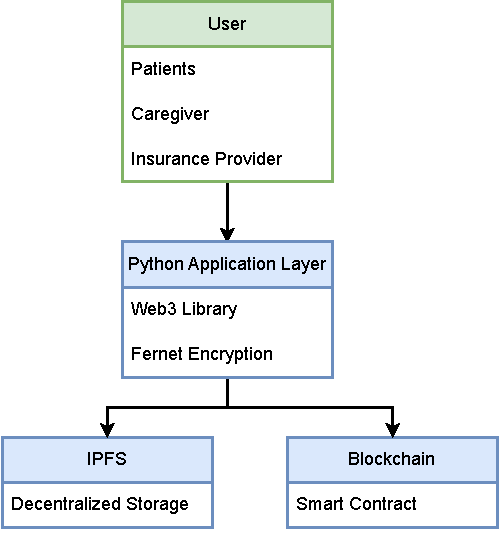
\includegraphics[width=0.5\columnwidth]{BlockChainPaper/Overview.pdf}
    \caption{General overview of system architecture. The Python Application acts as the intermediary, handling communication between IPFS and the blockchain smart contract. This architecture prevents direct communication between the user and both the smart contract and IPFS.}
    \label{fig:overview}
\end{figure}
By utilizing the Python Application Layer as the intermediary, the architecture efficiently manages data storage and access. The blockchain smart contract is optimized to store minimal yet crucial information: the Content Identifier (CID) for locating patient data within IPFS and the decryption keys needed for accessing this data. This method addresses the high costs and slow processing times associated with storing large volumes of data directly on the blockchain. Furthermore, it leverages the blockchain's strengths for secure, immutable transactions while utilizing IPFS for its scalable, decentralized data storage capabilities.

This bifurcated strategy allows the system to benefit from the security and immutability of blockchain technology for access management, while IPFS handles the heavy lifting of data storage, offering a solution that is both cost-effective and scalable. Thus, our system architecture not only prioritizes data security but also ensures that the system remains secured while having good quality of service.


\subsection{Core Components}

\begin{figure}[ht]
\centering
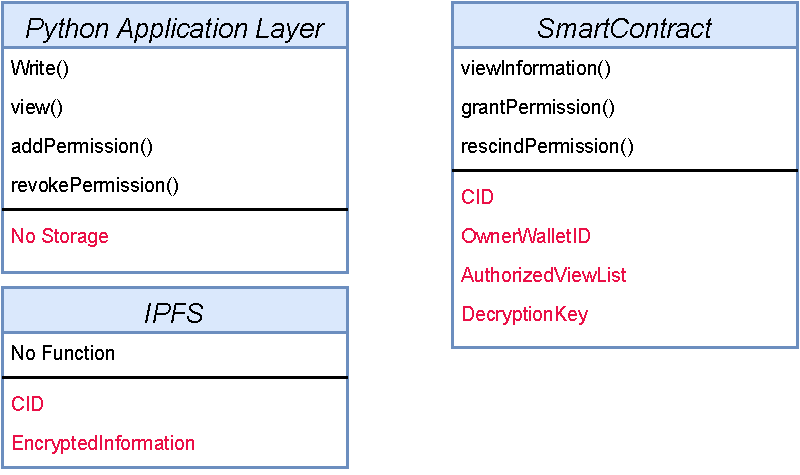
\includegraphics[width=0.7\columnwidth]{BlockChainPaper/ComponentOverview.pdf}
\caption{In this components overview, the Python application layers solely function as the user interface, offering various functionalities. Data storage doesn't occur at the application level. Instead, IPFS stores the Content Identifier (CID) and encrypted data. The smart contract retains the CID, wallet ID, authorized viewers, and decryption key, safeguarded by the blockchain wallet. Moreover, the system ensures data privacy by never exposing raw data.}
\label{fig:components}
\end{figure}

\subsubsection{IPFS}
The InterPlanetary File System (IPFS) \cite{ipfs2023} is fundamental to our EHR system, selected for its decentralized architecture, which mitigates the risks associated with centralized data storage systems. By leveraging a peer-to-peer network, IPFS ensures enhanced data resilience and widespread availability, distributing files across a global network of nodes. This approach not only strengthens the security and integrity of the data but also safeguards patient privacy by eliminating single points of control over the data.

IPFS's cost-effectiveness coupled with substantial community support further cements its role within our system. Operating as a free platform, it perfectly aligns with our vision for a cost-efficient, scalable EHR system devoid of exorbitant storage fees. Continuous development and support from its active community guarantee that IPFS stays on the cutting edge of decentralized storage solutions, making it the preferred choice for the secure handling of extensive patient records.

As depicted in Figure \ref{fig:components}, the decentralized and peer-to-peer nature of IPFS means universal accessibility with the correct Content Identifier (CID). To protect patient confidentiality and prevent unauthorized access to sensitive information, only encrypted patient EHR records are stored on IPFS. In our architecture, each patient's record is associated with a unique CID, positioning IPFS as a secure database. Users retrieve their encrypted information by providing the corresponding CID, maintaining privacy and security across the system.


\subsubsection{Blockchain and Smart Contract}
In the realm of blockchain technology, Ethereum\cite{ethereum2014} emerges as a platform offering advanced functionalities that surpass traditional cryptocurrency systems like Bitcoin. Ethereum's introduction of smart contracts—self-executing contracts with the terms of the agreement directly written into code—enables sophisticated applications across various sectors, notably in healthcare, where data integrity and access control are paramount. Opting for Ethereum as the backbone of our Electronic Health Records (EHR) system leverages these benefits to assure unparalleled security, integrity, and management flexibility for sensitive health data.

The utilization of blockchain technology within our EHR system introduces a high level of security and integrity, capitalizing on the inherent characteristics of blockchain that safeguard against unauthorized access and tampering. By ensuring that users maintain the privacy of their wallet's private key, the blockchain serves as an impregnable repository for extremely sensitive information, such as access permissions and ownership details of medical records.

To facilitate usage on the blockchain, we wrote a  smart contract, EHRContract, a self-executing program that operates autonomously on the blockchain. As illustrated in the pseudocode \ref{pseudocode} and Figure \ref{fig:components}, the smart contract is designed to manage critical aspects of the EHR system:

\begin{algorithm}
\caption{EHRContract: Electronic Health Records Smart Contract}
\begin{algorithmic}[1]

\State \textbf{Private Variables:}
\State \quad $owner$: Address of the contract creator
\State \quad $ehrCID$: String, unique identifier for EHR data
\State \quad $authorizedViewers$: List of addresses authorized to view EHR data
\State \quad $DecryptionKey$: Fernet decryption key used for data access

\Procedure{Constructor}{\_ehrCID: String, \_DecryptionKey: String}
    \State $owner \gets \text{current user}$
    \State $ehrCID \gets \_ehrCID$
    \State $DecryptionKey \gets \_DecryptionKey$
    \State Add $owner$ to $authorizedViewers$
\EndProcedure

\Procedure{grantPermission}{viewer: Address}
    \If{$\text{current user} = owner$}
        \State Add $viewer$ to $authorizedViewers$
    \EndIf
\EndProcedure

\Procedure{rescindPermission}{viewer: Address}
    \If{$\text{current user} = owner$}
        \State Remove $viewer$ from $authorizedViewers$ if present
    \EndIf
\EndProcedure

\Function{viewInformation}{}
    \If{$\text{current user} \in authorizedViewers$}
        \State \Return $ehrCID, DecryptionKey$
    \Else
        \State \Return "Access Denied"
    \EndIf
\EndFunction

\Function{isViewerAuthorized}{viewer: Address}
    \State \Return $viewer \in authorizedViewers$
\EndFunction

\end{algorithmic}
\label{pseudocode}
\end{algorithm}
This smart contract structure outlines the storage of the Content Identifier (CID) of patient records in IPFS, the decryption key for accessing these records, a list of viewers authorized to access the data (authorizedViewers), and the owner of the data. The functions grantPermission, rescindPermission, and viewInformation encapsulate the essence of our system's permission management, enabling the record owner to exert full control over who can access their medical records. Such functionality ensures that patients can dynamically manage access to their data, granting or rescinding permissions as needed with immediate effect.

The deployment of this smart contract within our EHR system architecture maximized user control over their medical records, enhancing patient autonomy and trust in the digital management of health information. By leveraging the immutable and decentralized nature of blockchain, our system not only secures sensitive medical data but also fosters a more transparent and accessible healthcare ecosystem.

\subsubsection{Python Application Layer}
Within our Electronic Health Records (EHR) system, the Python Application Layer fulfills two critical roles: it functions as both the user interface (UI) and the conduit for all interactions between the InterPlanetary File System (IPFS), the blockchain smart contract, and the end-users. Illustrated in Figure \ref{fig:components}, the operations facilitated by this layer closely correspond to those defined within the smart contract, with the notable inclusion of a write function. This strategic design ensures that user interactions, which might be complex if navigated directly through the smart contract and IPFS, are significantly simplified.

In addition to serving as an intermediary, this Python application is tasked with the responsibility of managing data encryption and decryption. For this purpose, it utilizes Fernet due to its straightforward application and effective data protection capabilities. Fernet's ease of implementation provides a security framework suitable for the prototype phase of our system. Nonetheless, we recognize that transitioning to a deployment ready for industry adoption may necessitate the integration of a more advanced encryption architecture. However, thanks to the modularity of the design, the transition process should be straight forward.



\subsection{User Roles and Interaction}

Our EHR system defines three primary user roles to effectively cater to the diverse interactions within the healthcare ecosystem: patients, caregivers (doctors), and insurance providers.

\begin{figure}[ht]
\centering
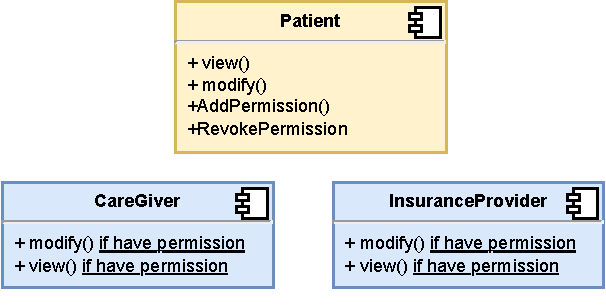
\includegraphics[scale=0.75]{BlockChainPaper/UserPermission.pdf}

\caption{Permissions overview, illustrating the specific capabilities assigned to patients, caregivers, and insurance providers within the EHR system.}
\label{fig:userPermission}
\end{figure}

As shown in Figure \ref{fig:userPermission}, the design prioritizes patient autonomy over their health records, allowing them comprehensive control, including read, write, and permission management capabilities. Caregivers and insurance providers are also enabled to view and modify EHRs, provided they have obtained explicit consent from the patient.

\begin{figure}[ht]
\centering
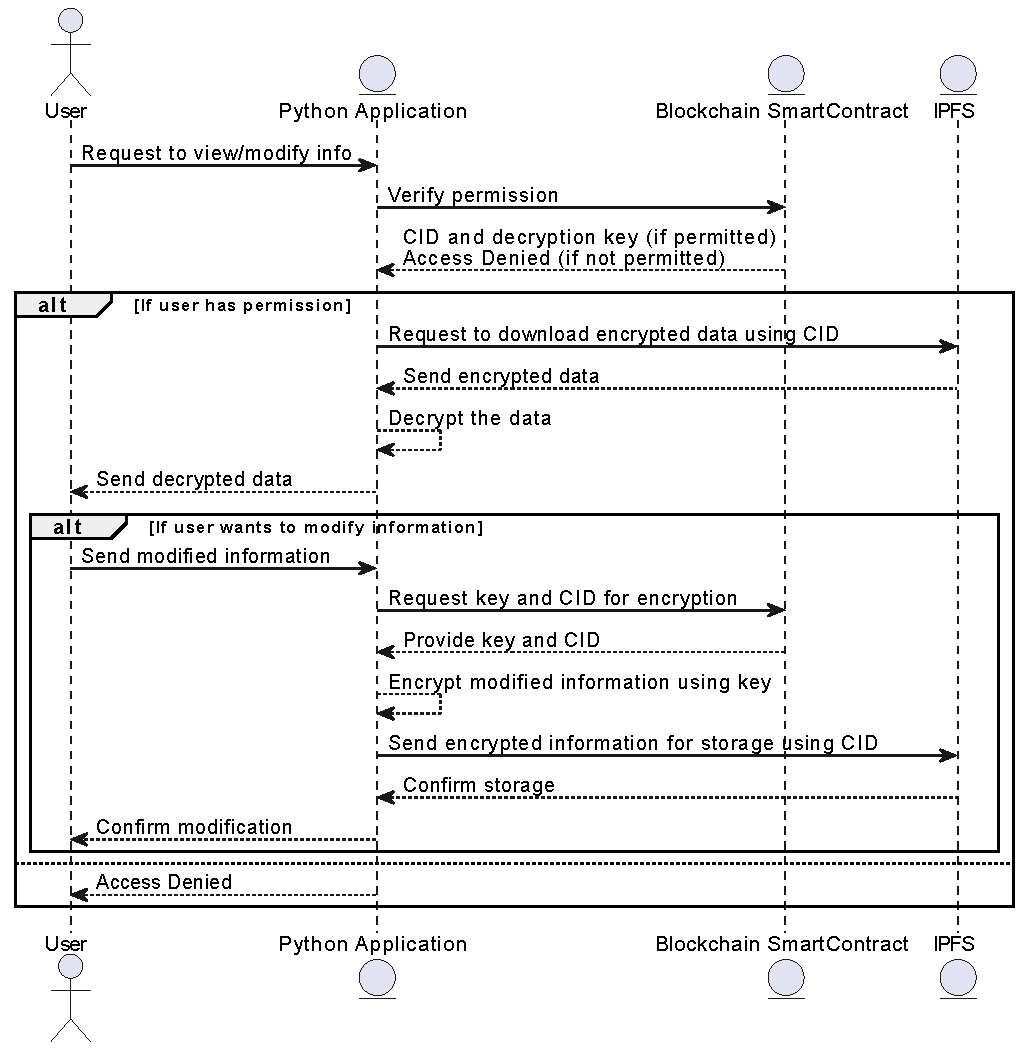
\includegraphics[width=0.8\columnwidth]{BlockChainPaper/ReadWriteProcess.pdf}
\caption{Flowchart depicting the sequence of operations in a typical read/write process within the EHR system, emphasizing the steps from user interaction to data retrieval or modification.}
\label{fig:readwrite}
\end{figure}

The process of interacting with the EHR system for reading or writing data involves several key steps, as outlined in Figure \ref{fig:readwrite}:

\begin{itemize}
  \item \textbf{Initial User Access:} Users first access the system through the Python application.
  \item \textbf{Authentication and Authorization:}
  \begin{itemize}
    \item The Python application queries the smart contract to verify user permissions.
    \item If unauthorized, the system displays an error message.
  \end{itemize}
  \item \textbf{Data Retrieval for Authorized Users:}
  \begin{itemize}
    \item Upon authorization, the smart contract provides the CID (Content Identifier) and decryption key.
    \item The Python application uses the CID to fetch the encrypted data from IPFS.
    \item The decryption key is then applied to decrypt the data, which is presented to the user.
  \end{itemize}
  \item \textbf{Data Modification (Write Requests):}
  \begin{itemize}
    \item Users make modifications to their EHR data within the Python application.
    \item The application requests the CID and decryption key from the smart contract for the data to be modified.
    \item After user modifications, the Python application encrypts the data using the same Fernet key (due to Fernet's symmetric encryption).
    \item The newly encrypted data is uploaded back to IPFS, completing the write process.
  \end{itemize}
\end{itemize}


\subsection{Dataset and Processing}

\subsubsection{Synthea}

In our endeavor to meticulously address privacy and ethical concerns associated with the use of real-life patient data, particularly in light of its exposure to IPFS, we have chosen to employ the Synthea dataset. Synthea\cite{synthea2017}, an open-source software tool, is adept at generating synthetic but remarkably realistic patient health records. It crafts detailed medical histories that closely replicate the format, structure, and content of genuine EHRs—encompassing demographics, allergies, medications, and various medical encounters. This capacity renders Synthea an exemplary substitute for actual patient data within our blockchain-based EHR system. Our project specifically utilized '1K Sample Synthetic Patient Records, CSV' obtained from Synthea.

\begin{figure}[ht]
\centering
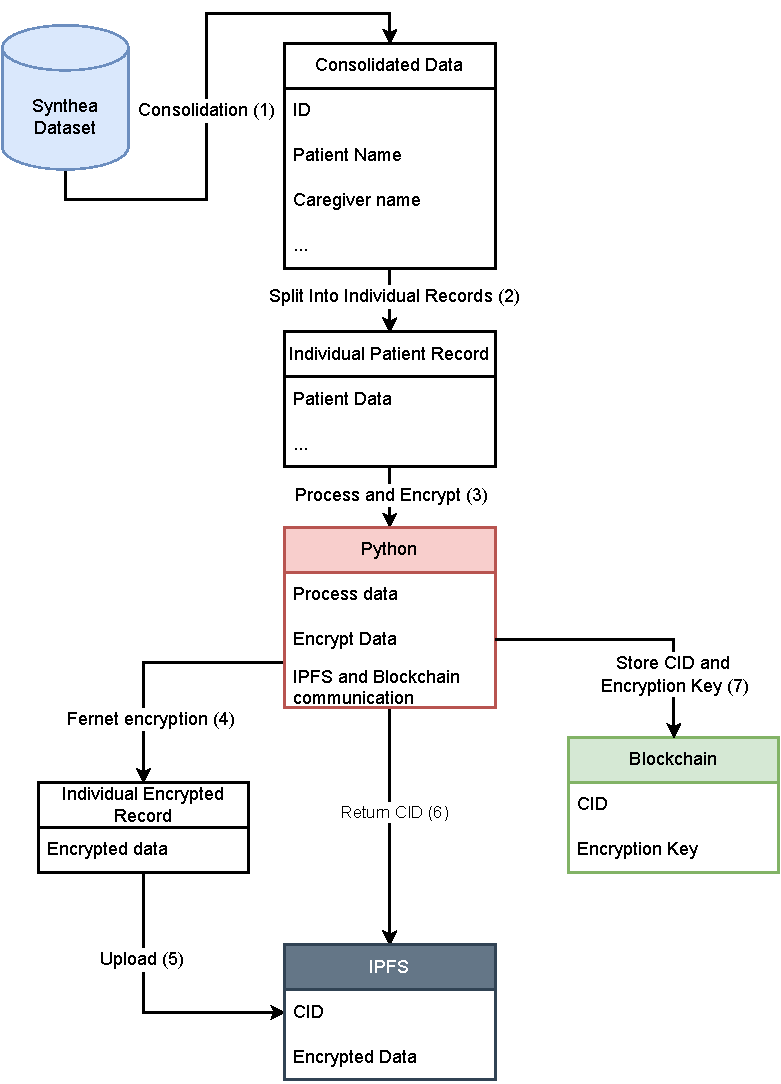
\includegraphics[scale=0.75]{BlockChainPaper/DataProcessing.pdf}
\caption{Illustration of the data processing workflow, from sourcing synthetic patient records from Synthea to encrypting and storing these records on IPFS, and finally integrating with the blockchain.}
\label{fig:dataProcessing}
\end{figure}

Figure \ref{fig:dataProcessing} delineates the comprehensive process we employed for data handling. The procedure involves several critical steps:

\begin{itemize}
\item \textbf{Data Consolidation:} Synthea's extensive and detailed dataset is consolidated into a singular table that encapsulates key patient information, including identifiers such as Id, First Name, Last Name, Insurance Provider, and Caregiver details.

\item \textbf{Data Segmentation:} This unified table is then segmented into multiple CSV files, with each file representing a unique patient ID, thereby individualizing the records.

\item \textbf{Encryption:} Each patient record is encrypted using a randomly generated Fernet key, ensuring the security of the data during transmission and storage.

\item \textbf{Storage on IPFS:} The encrypted files are uploaded to IPFS, which assigns a Content Identifier (CID) to each file, indicating its unique location within the IPFS network.

\item \textbf{Blockchain Integration:} Finally, the CID, the encryption key, and the patient's wallet ID are incorporated into the constructor of our smart contract and deployed on the blockchain. This step effectively binds the patient's identity with their medical record in a secure, immutable manner.
\end{itemize}


\subsection{Testing and Evaluation}

To thoroughly evaluate the performance of our system, we focused on its two main components: IPFS and blockchain. Initial testing on IPFS revealed that data retrieval times are exceptionally fast, typically under 0.3 seconds, which can be considered nearly instantaneous. This efficiency led us to concentrate our testing efforts on the blockchain component, specifically the performance of our smart contract.

Our smart contract incorporates three essential functions: \texttt{view()}, \texttt{addPermission()}, and \texttt{rescindPermission()}. Given that the \texttt{view()} function incurs no cost and is uniformly swift across blockchain networks, our performance evaluation targeted the \texttt{addPermission()} and \texttt{rescindPermission()} functions. We measured two key performance metrics: transaction cost (in Ether) and transaction time (in seconds) for each operation.

For a realistic assessment of performance under stress conditions, we deployed our smart contract on Sepolia\cite{sepoliaTestnet2022}, a live test network known for its high traffic. However, it's important to recognize that results from Sepolia might not fully represent real-world usage of our EHR system, as Sepolia experiences a wide range of traffic globally, most of which is unrelated to EHR records. To complement our testing on Sepolia and simulate a more controlled environment, we also deployed our system on a local blockchain network using Ganache. This allowed us to evaluate performance in an isolated setting, free from external network traffic.

Performance tests were conducted with 30 runs per hour throughout the day to account for potential variations in network traffic and its impact on transaction times and costs. This approach ensures that our evaluation captures both worst-case scenarios on a busy test network like Sepolia and ideal conditions on a dedicated local network, providing a better view of our system's performance capabilities.

\section{Results}

\subsection{Sepolia Testnet}

\begin{figure}[ht]
\centering
\resizebox{\columnwidth}{!}{%
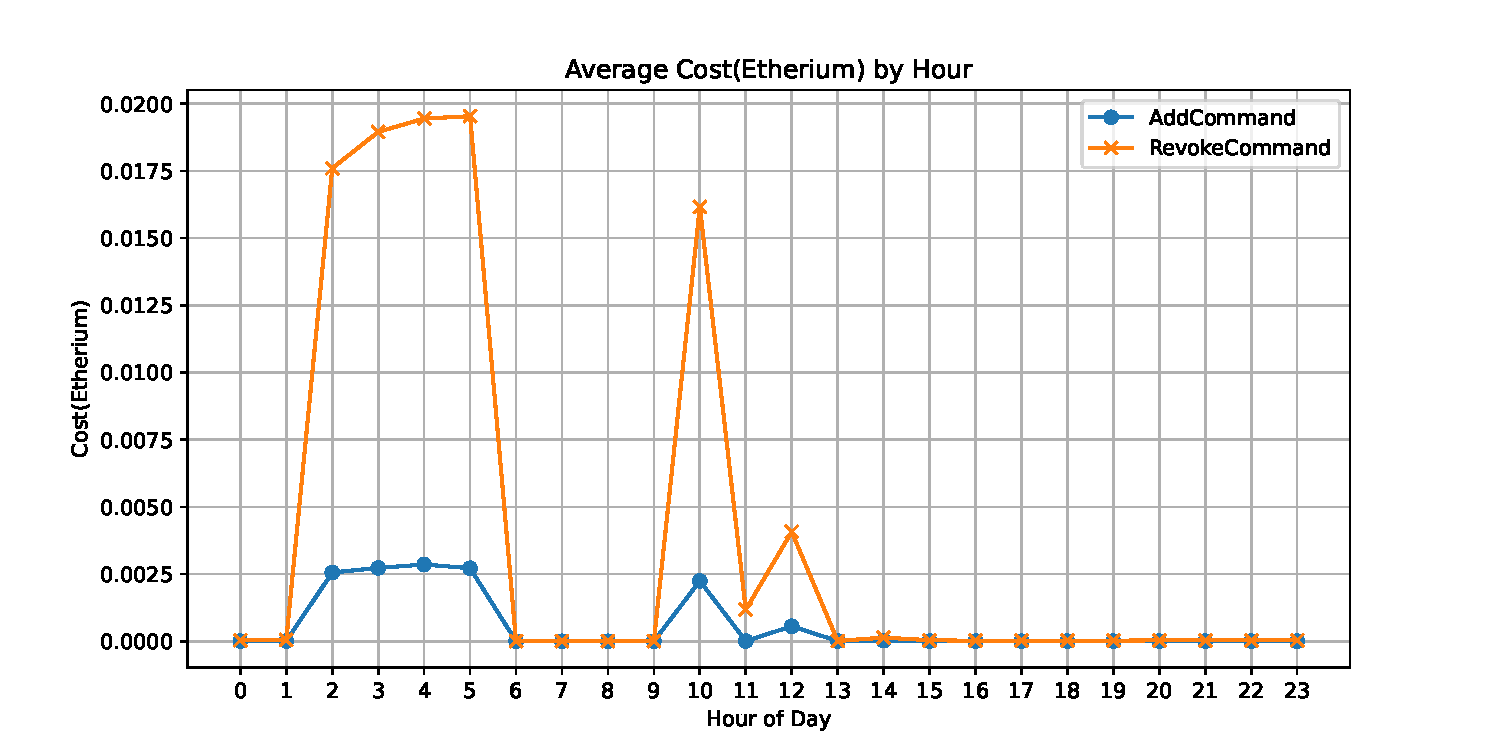
\includegraphics[width=0.8\columnwidth]{BlockChainPaper/Sepholia_transaction_cost_plots.pdf}
}
\caption{Transaction Cost Performance on Sepolia Throughout the Day}
\label{fig:Seph_Cost}
\end{figure}

\begin{figure}[ht]
\centering
\resizebox{\columnwidth}{!}{%
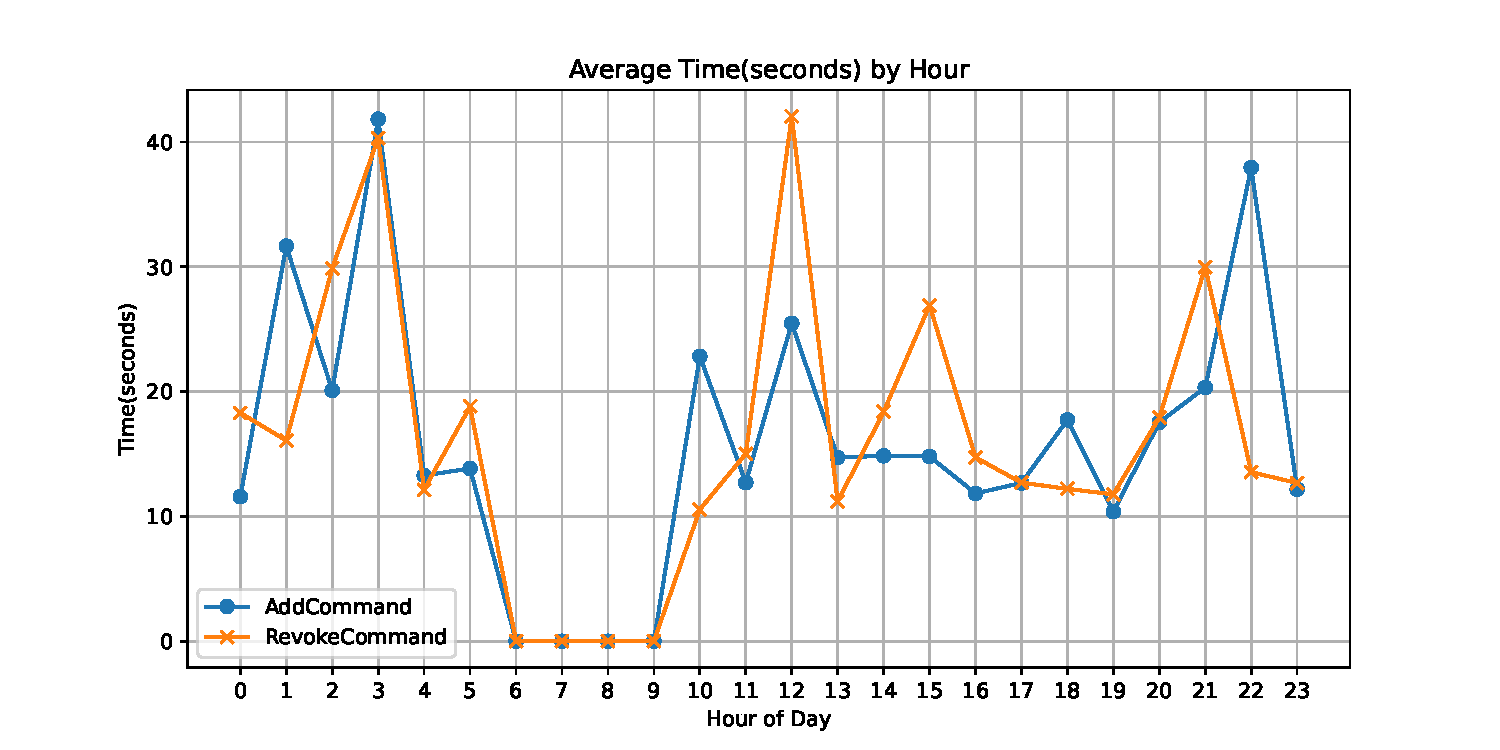
\includegraphics[width=0.8\columnwidth]{BlockChainPaper/Sepholia_transaction_time_plots.pdf}
}
\caption{Transaction Time Performance on Sepolia Throughout the Day}
\label{fig:Seph_Time}
\end{figure}

Analysis of the Sepolia Testnet reveals distinct patterns in transaction costs and times for "Add" and "Revoke" commands, marked by significant fluctuations at specific periods, especially during peak hours. The network experiences notable congestion between 6 AM and 9 AM North American Central Time Zone (CT), resulting in transaction failures under our configured wallet settings.

Figure \ref{fig:Seph_Cost} illustrates the varying transaction costs for "Add" and "Revoke" commands. Peak network activity spans from 1 AM to 1 PM North American Central Time Zone (CT), with "Revoke" transaction costs peaking at 0.019805 ether at 2 AM, and "Add" transactions reaching up to 0.0029 ether. Notably, the costs associated with "Revoke" commands are consistently higher than those for "Add" commands, reflecting the network's prioritization of resource allocation towards the revocation processes.

Figure \ref{fig:Seph_Time} displays the fluctuation in transaction times, where the fastest times recorded for "Add" commands are around 8.84 seconds, and for "Revoke" commands, approximately 12.01 seconds. Nonetheless, transaction durations generally exceed 10 seconds, with peaks at 107.99 seconds for "Revoke" commands at 1 AM and 55.09 seconds for "Add" commands at 12 PM, coinciding with the highest traffic volumes. These peaks in transaction times during early morning hours can be attributed to the global nature of blockchain networks, where nighttime in one region corresponds to daytime in another, leading to non-uniform network usage.

This analysis highlights the system's performance under stress, particularly during live network testing, where some transactions failed due to settings that did not account for peak congestion times. Such prolonged transaction durations are impractical for EHR operations, especially in scenarios demanding rapid access to healthcare data. This variability underscores the importance of further testing and optimization, particularly in more controlled environments like Ganache, to ensure the system's reliability and efficiency in real-world healthcare applications.

\subsection{Ganache Results}

\begin{table}[ht]
\centering
\begin{tabular}{lcc}
\hline
Operation & Average Time (seconds) & Average Cost (Ether) \\
\hline
Add Permission & 0.052096 & 0.00099022 \\
Revoke Permission & 0.070517 & 0.00119175 \\
\hline
\end{tabular}
\caption{Average Transaction Time and Cost for Operations on Ganache}
\label{tab:Ganache}
\end{table}

\begin{figure}[ht]
\centering
\resizebox{\columnwidth}{!}{%
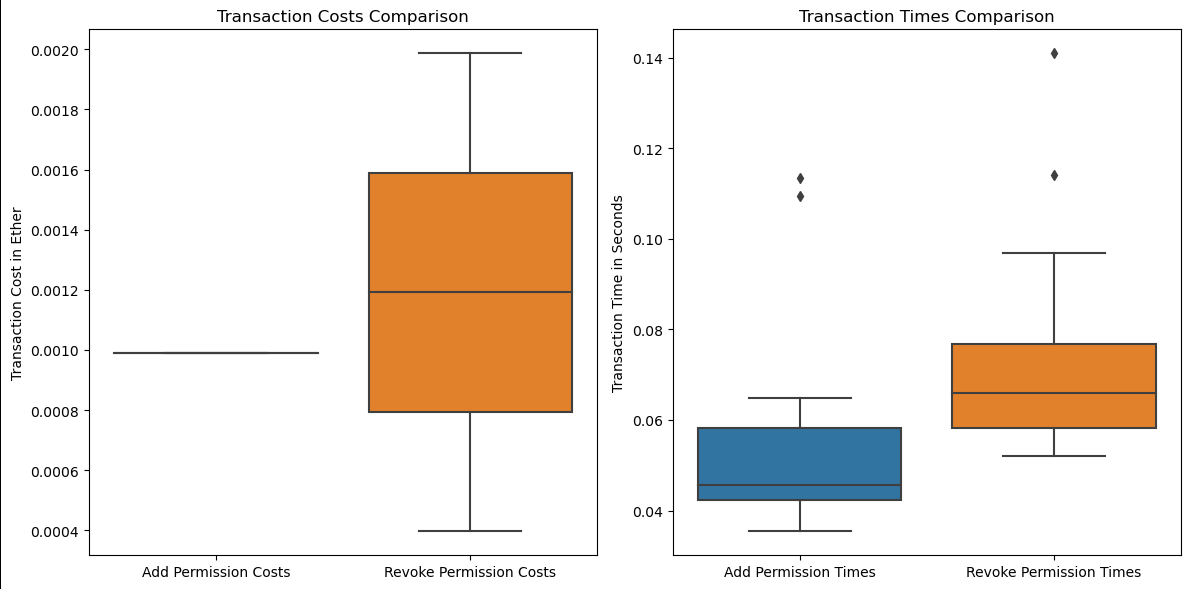
\includegraphics[width=0.8\columnwidth]{BlockChainPaper/GanacheBoxPlot.png}
}
\caption{Ganache's Box Plot Performance}
\label{fig:Ganache}
\end{figure}

The data in Table \ref{tab:Ganache} and Figure \ref{fig:Ganache} demonstrate the system improvements with Ganache. Adding permissions is achieved in an average time of $0.052096$ seconds at a cost of $0.00099022$ Ether. Revoking permissions, slightly more resource-intensive, is completed in $0.070517$ seconds at a cost of $0.00119175$ Ether.

Figure \ref{fig:Ganache} offers insights into Ganache's model performance, showing consistent costs for adding permissions and variable costs for revocation tasks. Additionally, transaction times for adding permissions are generally lower, indicating that revoking permissions is a more complex task for the network.

One thing to note is that performance in Ganache is extremely consistent, as reflected in the add permission cost, where there is close to no variation. While this might point to Ganache as a better platform, it might not be the case as we are only having the blockchain on a single node for testing. Thus, the consensus mechanism, cost, and effectiveness are much quicker and more efficient. More testing should be done in the future for larger networks. However, we still want to include the result to show the potential of our novel approach when there is a dedicated network for Electronic Health Records (EHR) on blockchain.

\section{Discussion}

Our study demonstrates the potential for implementing Electronic Health Records (EHR) on a blockchain system, transitioning from traditional databases. Utilizing the InterPlanetary File System (IPFS) enhances scalability for extensive EHR data storage, complementing blockchain's advantages. Results indicate our approach is promising, delivering cost-effective and fast services (less than 0.1 seconds for all tasks) in a private Ethereum network like Ganache.

Future research should address:

\begin{enumerate}
    \item Network implementation: The configuration and traffic significantly affect service quality. While Ganache shows excellent performance in ideal conditions, extensive load testing is necessary to determine if Ethereum is suitable or if a new network with different consensus mechanisms must be developed for optimal performance.
    
    \item Patient-Centric Architecture: Focusing on security and privacy raises challenges, especially when patients cannot grant data access, potentially leaving healthcare professionals without crucial information. This issue necessitates developing delegation mechanisms and fostering collaboration among medical professionals and patients.
\end{enumerate}


\section{Conclusion}

In conclusion, our study demonstrates the practical implementation of blockchain technology in Electronic Health Record (EHR) systems, addressing centralization, standardization, and security challenges. The integration of blockchain and the InterPlanetary File System (IPFS) establishes a secure and scalable foundation for healthcare data management.

While our results are promising, they highlight two key areas for future research. Patient-centric design requires solutions for scenarios where patients cannot grant access. Further optimization of the blockchain's network is essential, especially with system scalability in mind.

Blockchain, when combined with IPFS, offers a viable alternative for contexts where privacy and security are paramount. This hybrid approach harnesses blockchain's strengths while mitigating its limitations, extending its potential to various database applications in addition to EHR systems.

\chapter[Learning from Supply-Chain Disruptions (Pre- and Post-COVID)]{Learning from Supply-Chain Disruptions (Pre- and Post-COVID)}\label{chap:supplychain}

\noindent\emph{Chapter bridge.} The two chapters that follow rest on a premise:
that data drawn from different institutions, or from the same institution under
different operating conditions, is distributed differently enough to break a model
trained on any one slice---the non-IID problem that gives consent churn its
teeth in Chapter~\ref{chap:fl_clusters}. This chapter supplies real-world evidence
for that premise. Modeling delivery lead time across a large multi-institutional
health-commodity supply chain, it shows that the features driving the model
\emph{shift} between normal and pandemic operating regimes---a documented
distribution shift across conditions, the operational analog of the cross-silo
heterogeneity the federated study must withstand. It also contributes the
regression-and-feature-importance evaluation discipline reused later. The
supply-chain domain is treated here as motivating evidence, not as a second
modeling contribution. This chapter is adapted from the candidate's published
work~\cite{nhan2024optimizing}.

\section{Introduction}
\label{sec:introduction}

Supply chain management has always been a critical area of study. It not only reduces costs from production to delivery but also decreases the time it takes for products to reach customers—known as lead time. In a globalized world, the efficiency of supply chains is even more important. While there is extensive literature on supply chain management in business, research on supply chains in the healthcare domain is comparatively scarce. A literature review spanning from 2000 to 2018 highlights just 43 papers \cite{beldek2020supply}, which is minimal given the 18-year time frame.

This is a significant issue as "The global pharmaceutical industry directly contributed 532 billion U.S. dollars of gross value added to the world’s GDP in 2017. This equals one percent of global GDP or about the GDP of the Netherlands \cite{wifor2020}." Given the substantial economic impact of the healthcare and pharmaceutical industries, there should be a greater focus on improving supply chain systems. A more efficient supply chain in healthcare not only reduces costs for patients but also ensures timely delivery of essential items. A good predictive model is crucial in this context as it can help anticipate delays and inefficiencies, allowing for proactive measures to mitigate risks. This can ultimately enhance the reliability and responsiveness of healthcare supply chains, ensuring better outcomes during critical times.

The COVID-19 pandemic has particularly exposed the vulnerabilities in healthcare supply chains, leading to significant losses in lives due to a lack of resilience. In response to this, our research aims to take a closer look at the supply chain for health commodity aid. The aim is not only to develop a reasonable accurate predictive model that can help with the prediction of lead time but also to identify and analyze the factors that affect final lead times during both normal and pandemic periods.

\section{Background}

While the combination of machine learning technologies and supply chain management techniques in the healthcare domain is rather underexplored, there are still some results that stand out. Primarily, most research that we looked at generally focuses on two categories: technical efficiency improvement and risk management/resilience.

\subsection{Technical Efficiency Improvement}

\begin{itemize}
  \item \textbf{Digitalization through ERP Systems}
  
  The paper "Digitalization of the Healthcare Supply Chain through the Adoption of Enterprise Resource Planning (ERP) Systems in Hospitals: An Empirical Study on Influencing Factors and Cost Performance" \cite{ERPSupplyChain} explores the adoption of ERP systems in hospitals, showing significant potential in reducing supply chain costs and improving operational efficiency. This study demonstrated that technological and organizational readiness, hospital size, governmental policies, and perceived benefits significantly influence ERP adoption. These systems enhance operational efficiency and financial performance by integrating technology into hospital operations, leading to better resource management and cost savings.
  
  \item \textbf{IoT-Enabled Solutions}
  
  The paper "Enhancing Medicine Supply Chain Efficiency in Rural African Healthcare through IoT-Enabled Smart Mobile Medicine Storage" \cite{IotHealthCareSupplyChain} proposed the use of IoT (Internet of Things, micro devices, sensors) to improve the efficiency of medicine supply chains, particularly in rural and underserved areas. The research successfully designed and implemented a smart mobile medicine storage box that monitors environmental conditions both inside and outside the box. This IoT-enabled smart medicine storage box ensures the quality and safety of pharmaceuticals by monitoring environmental conditions in real-time and updating the information to the web. This system allows workers to monitor both the location and weather conditions and notifies the responsible party to take action when necessary. This model helps prevent drug wastage and ensures effective healthcare delivery in remote regions.
  
  \item \textbf{Blockchain Technology}
  
  The systematic literature review titled "Blockchain for the Healthcare Supply Chain: A Systematic Literature Review" \cite{BlockChainHeathCare} explores the current research on how blockchain technology can be used in the healthcare domain. Blockchain is particularly useful due to its inherent security features and the application of smart contracts, which automate transactions between peers under user-defined conditions, leading to more efficient systems. However, most of the existing research is still in the modeling stage and has not been implemented in real-life applications. Therefore, further research with practical applications is needed to truly demonstrate the usefulness of blockchain in the healthcare sector.
  
  \item \textbf{Machine Learning Applications}
  
  The paper "Estimating Lead Time Using Machine Learning Algorithms: A Case Study by a Textile Company" \cite{MachineLearningLeadtime} used data from a textile company to create a model to try to predict lead time. Their results show the potential application of machine learning models in lead time prediction, where the bagging and random forest models achieved an R\textsuperscript{2} value of 0.84 or higher and had low predictive error.
\end{itemize}

\subsection{Supply Chain Resilience and Risk Management}

\begin{itemize}
  \item \textbf{Advanced Performance Evaluation Techniques}
  
  The paper "Forecasting Sustainability of Healthcare Supply Chains Using Deep Learning and Network DEA" \cite{ForcastDeepLearning} proposed the combination of Network Data Envelopment Analysis (NDEA) with deep learning techniques to forecast and optimize the sustainability of healthcare supply chains. This model can potentially help scholars identify inefficiencies and predict future performance, aiding in better decision-making and resource allocation. Such advanced techniques are important for enhancing the resilience of healthcare supply chains.
  
  \item \textbf{Risk Management and Circular Economy}
  
  The paper "Upstream Healthcare Supply Chain Risk Management in the Implementation of Circular Economy at the Primary Care Level" \cite{UpstreamRiskManagement} acknowledges the need to reduce the impact of supply chain disruptions and healthcare waste. The authors propose implementing circular economy principles to identify and mitigate risks like supply delays and product shortages. Using Failure Mode Effect and Critical Analysis, the study prioritizes risks, showing that delays or shortages of critical products, such as latex gloves, often due to import delays, have the highest Risk Priority Number. To address this, the study suggests diversifying suppliers and using biodegradable materials like green nitrile gloves. This approach highlights the importance of supplier and manufacturer innovation in New Product Development stages to promote sustainable development.
  
  \item \textbf{Pandemic Response and Vaccine Distribution}
  
  The COVID-19 pandemic has been difficult for every country. One example is shown in the paper titled "Insight Importance of Supply Chain Management of Vaccines in India During Covid Pandemic" \cite{IndiaCovid19Vacc}, where it explores the critical components and challenges of vaccine supply chain management in India. It emphasizes the importance of efficient cold chain facilities and highlights issues such as population size affecting distribution, with smaller states managing more effectively despite proportional increases in health workers. The study also notes disparities in booking vaccination slots, with older individuals finding it easier than younger ones, and an overall smoother process for second doses.
  
  A more effective distribution system is needed. One suggestion comes from the paper "A Comprehensive Blockchain Framework for (COVID-19) Vaccine Program Registration, Supply Chain, and Side Effects" \cite{BlockchainCovid19Vacc}, which proposes a blockchain-based system to address vaccine distribution and monitoring challenges. It suggests integrating vaccine supply chain management with beneficiary registration and side-effect tracking using blockchain technology to ensure traceability and secure data sharing. The framework aims to link cold supply chain data with side-effect information and registration records to identify issues related to manufacturing or distribution.
\end{itemize}

While there has been significant research on supply chain efficiency and resilience, particularly during the pandemic, there is a notable lack of studies combining the use of machine learning models to predict lead times and really understand the difference between normal and pandemic operation. One study that examines the resilience of supply chain systems pre- and post-COVID in the healthcare domain is "A large-scale real-world comparative study using pre-COVID lockdown and post-COVID lockdown data on predicting shipment times of therapeutics in e-pharmacy supply chains" \cite{pre-postCovid-study}. In this research, the authors used various machine learning models to predict shipment time, achieving 93.5\% accuracy on post-COVID data and 91.35\% on pre-COVID data. This study shows the potential for using machine learning in this field. However, there are some oversights that we plan to expand upon in our study:

\begin{itemize}
  \item Utilization of shipment time instead of lead time: While shipment time is an important metric, when looking at pre- and post-pandemic periods, many factors affect the supply chain. Thus, we believe that lead time is a better metric.
  \item Choice of classification model instead of regression model: In the original paper, the authors chose binary classification (on-time/early delivery and late delivery). A downside to the binary approach is its inability to capture the true degree of delay. A one-day delay can be an inconvenience, while a three-month delay is disruptive and potentially life-threatening. We address this issue by using a regression model.
  \item Lack of comparison between the features' importance of the model pre- and post-pandemic. This is important to study as we should know what differs in the normal vs. pandemic periods.
\end{itemize}

Acknowledging these gaps, our research aims to develop a regression model capable of accurately predicting lead times for both pre- and post-COVID periods. The goal is not to replace human prediction but to provide an additional reference point that can be used alongside human predictions, creating a comprehensive range for downstream supply chain planning. Additionally, we aim to analyze the differences in feature importance between these two periods to understand variations in supply chain operations, thereby offering insights for optimization.

\section{Methodology}
\label{sec:methodology}
\subsection{Dataset}
The dataset employed for this study is the "USAID Global Health Supply Chain Program - Procurement and Supply Management (GHSC-PSM) Health Commodity Delivery Dataset" \cite{dataset}. This dataset is made up of detailed records of health commodity orders delivered through the USAID GHSC-PSM project with agree delivery year from 2015 to 2025. It includes orders funded by various programs such as PEPFAR, PMI, family planning/reproductive health, maternal and child health, COVID-19, and other USAID and USG initiatives.

\subsection{Preprocessing}

Originally, the dataset contained 38,500 rows and 104 columns. However, the data presented significant challenges due to its messiness and a high incidence of missing values (NaNs). To address these issues, we organized the products by categories and substituted missing values with the median of each feature set. Subsequently, we dropped all rows with remaining NaNs, reducing the dataset to approximately 16,000 rows. A conscious decision was made not to remove outliers, as our goal is to develop a resilient model that can account for extreme values, such as those observed during pandemic times.

For analysis, we condensed the original 104 columns into a more manageable set of features deemed most relevant for this study. Below is a breakdown of the selected features categorized into `categories` and `numeric` types, along with the `target` variable:


\begin{longtable}{|l|p{10cm}|}
\hline
\textbf{Category} & \textbf{Features/Variables} \\ \hline
\endfirsthead
\hline
\multicolumn{2}{|c|}{{\tablename~\thetable{} -- continued from previous page}} \\ \hline
\textbf{Category} & \textbf{Features/Variables} \\ \hline
\endhead
\hline \multicolumn{2}{|r|}{{Continued on next page}} \\ \hline
\endfoot
\hline
\endlastfoot
Categorical Variables & Country, Transportation Mode, Order Type, Fulfillment Method, Product Category, Vendor Incoterm, Reason Code, Item Tracer Category, Framework Contract \\ \hline
Numeric Variables & Manufacture, Pick Up, Quality Assurance, Illustrative Price, RO Validation, Sourcing and Planning, USAID Approval, Process PO/DO, Reason Code Duration \\ \hline
Target Variable & Actual Lead Time (calculated from "Latest Actual Delivery Date" - "Order Entry Date") \\ \hline
\end{longtable}

After preprocessing, we examined the Variance Inflation Factor (VIF) to assess multicollinearity. VIF measures how much the variance of a regression coefficient is inflated due to multicollinearity. Values above 10 generally indicate high multicollinearity, which could potentially distort the model estimates.

\begin{table}[h!]
\centering
\begin{tabular}{|l|r|}
\hline
\textbf{Variable} & \textbf{VIF} \\ \hline
Manufacture & 2.100547 \\ \hline
Pick Up & 3.104425 \\ \hline
Quality Assurance & 2.176681 \\ \hline
Illustrative Price & 1.015987 \\ \hline
RO Validation & 1.501254 \\ \hline
Sourcing and Planning & 2.513305 \\ \hline
USAID Approval & 1.111466 \\ \hline
Process PO/DO & 1.650779 \\ \hline
Reason Code Duration & 1.137324 \\ \hline
\end{tabular}
\caption{Variance Inflation Factors (VIF) for Different Variables}
\label{table:vif}
\end{table}

\noindent
The VIF values for all numerical columns are well below the threshold of 10, indicating that multicollinearity is not a concern for our selected features. This ensures the stability and reliability of our regression coefficients. With the data satisfactorily preprocessed, we can confidently proceed to the analysis phase.

\subsection{Experiment Setup}
The primary goal of this project is to understand the impact of COVID-19 on the medical supply chain process. To achieve this, we initially aim to develop a predictive model that is accurate enough to facilitate further analysis, with an objective to maintain an error rate of around 7 days.

\subsubsection{Model Selection}
During initial testing, various models were evaluated based on their fit to the dataset, using the R-squared (R\textsuperscript{2}) metric to assess each model's performance. The Random Forest algorithm seems to be the most suitable due to its high average R\textsuperscript{2} value on the whole dataset. Random Forest is particularly effective for this dataset as it handles sparse data well and does not assume linearity in the data relationships. This model works by constructing multiple decision trees during training time and outputting the mean prediction of the individual trees, thus reducing overfitting and increasing prediction accuracy.

\subsubsection{Data Segmentation}
To assess the impact of COVID-19, the data was segmented into different periods for comparison:
\begin{itemize}
  \item \textbf{Before and After COVID-19:} Data was divided into two segments, before January 1, 2020, and after January 1, 2020, to analyze the changes in the supply chain dynamics due to the pandemic onset.
  \item \textbf{During Peak and Non-Peak COVID-19:} The dataset was also segmented into peak COVID-19 period (January 1, 2020, to March 22, 2022—the last day of the mask mandate in the US) and non-peak periods to understand fluctuations during the height of the pandemic.
\end{itemize}

\subsubsection{Performance Evaluation}
Each dataset segment was fitted to the Random Forest model, and performance metrics such as minimum error, maximum error, median error, Root Mean Square Error (RMSE), and R\textsuperscript{2} were calculated. This process was repeated 10 times with 10 shuffles of the dataset.

Upon obtaining the model results, the top five most important features were analyzed to understand their impact on the supply chain during the pandemic. This analysis aims to pinpoint which factors were most affected by COVID-19 and how they influenced the overall supply chain resilience.

\section{Results and Discussion}
\label{sec:results}
\subsection{USAID's Manual Expected Lead Time}
Before analyzing the results from our predictive model, we examined the errors in the manual expected lead times provided by USAID. The dataset includes the column 'Estimated Delivery Date'. We subtracted this column from the 'Order Entry Date' to calculate the 'Expected Lead Time'. We then assessed the variance between the predicted lead time and the 'Actual Lead Time', as shown in Table \ref{tab:error_metrics}.

\begin{table}[H]
\centering
\begin{tabular}{|l|r|r|r|r|r|}
\hline
\textbf{Period} & \textbf{Min\_Error} & \textbf{Max\_Error} & \textbf{Mean\_Error} & \textbf{Median\_Error} & \textbf{RMSE} \\
\hline
Whole Period     & 0.0 & 639.0 & 29.938709 & 0.0 & 906.910365 \\
After COVID-19   & 0.0 & 403.0 & 50.529947 & 0.0 & 1,176.568441 \\
Before COVID-19  & 0.0 & 639.0 & 13.990051 & 0.0 & 622.359383 \\
Peak Period      & 0.0 & 403.0 & 60.971333 & 0.0 & 1,302.676753 \\
Non-Peak Period  & 0.0 & 639.0 & 12.786385 & 0.0 & 582.361095 \\
\hline
\end{tabular}
\caption{Error Metrics for Different Periods by USAID Manual Prediction}
\label{tab:error_metrics}
\end{table}

Overall, the results are promising from a median perspective, indicating effective planning. However, during the pandemic, the errors are significantly higher, suggesting that standard planning methods may not adequately consider resilience in unpredictable situations.

\subsection{Fitment}

\begin{table}[h!]
\centering
\begin{tabular}{|l|l|r|r|r|r|r|}
\hline
\textbf{Metric} & \textbf{Period} & \textbf{Mean} & \textbf{Std Dev} & \textbf{Min} & \textbf{50\%} & \textbf{Max} \\ \hline
Min Error & After COVID & 0.00 & 0.00 & 0.00 & 0.00 & 0.00 \\ \cline{2-7}
 & Before COVID & 0.00 & 0.00 & 0.00 & 0.00 & 0.00 \\ \hline
Max Error & After COVID & 323.06 & 48.66 & 252.56 & 321.26 & 391.58 \\ \cline{2-7}
 & Before COVID & 559.25 & 98.36 & 395.62 & 633.05 & 645.75 \\ \hline
Average Error & After COVID & 16.44 & 0.83 & 15.41 & 16.63 & 17.47 \\ \cline{2-7}
 & Before COVID & 24.25 & 0.89 & 23.02 & 24.29 & 26.38 \\ \hline
Median Error & After COVID & 5.40 & 0.33 & 4.73 & 5.51 & 5.78 \\ \cline{2-7}
 & Before COVID & 8.90 & 0.42 & 8.14 & 8.99 & 9.70 \\ \hline
RMSE & After COVID & 33.59 & 1.84 & 30.47 & 33.85 & 36.20 \\ \cline{2-7}
 & Before COVID & 48.19 & 2.23 & 44.99 & 47.60 & 52.44 \\ \hline
R-squared & After COVID & 0.93 & 0.01 & 0.92 & 0.93 & 0.94 \\ \cline{2-7}
 & Before COVID & 0.88 & 0.01 & 0.87 & 0.89 & 0.89 \\ \hline
\end{tabular}
\caption{Comparison of Error Metrics Before and After COVID-19}
\label{table:before_and_after}
\end{table}

\begin{table}[h!]
\centering
\begin{tabular}{|l|l|r|r|r|r|r|}
\hline
\textbf{Metric} & \textbf{Period} & \textbf{Mean} & \textbf{Std Dev} & \textbf{Min} & \textbf{50\%} & \textbf{Max} \\ \hline
Min Error & Peak Pandemic & 0.00 & 0.00 & 0.00 & 0.00 & 0.00 \\ \cline{2-7}
 & Non-Peak & 0.00 & 0.00 & 0.00 & 0.00 & 0.00 \\ \hline
Max Error & Peak Pandemic & 314.95 & 67.03 & 229.18 & 292.79 & 401.79 \\ \cline{2-7}
 & Non-Peak & 487.80 & 105.85 & 365.86 & 459.22 & 646.35 \\ \hline
Average Error & Peak Pandemic & 18.12 & 0.65 & 16.61 & 18.20 & 18.81 \\ \cline{2-7}
 & Non-Peak & 22.99 & 0.58 & 22.07 & 22.82 & 23.93 \\ \hline
Median Error & Peak Pandemic & 5.99 & 0.55 & 5.10 & 5.92 & 7.00 \\ \cline{2-7}
 & Non-Peak & 8.17 & 0.52 & 7.17 & 8.21 & 9.19 \\ \hline
RMSE & Peak Pandemic & 36.76 & 2.08 & 32.22 & 37.11 & 39.90 \\ \cline{2-7}
 & Non-Peak & 45.56 & 1.17 & 43.37 & 45.45 & 47.65 \\ \hline
R-squared & Peak Pandemic & 0.92 & 0.01 & 0.91 & 0.92 & 0.94 \\ \cline{2-7}
 & Non-Peak & 0.89 & 0.01 & 0.88 & 0.89 & 0.90 \\ \hline
\end{tabular}
\caption{Comparison of Error Metrics During Peak and Non-Peak Pandemic Periods}
\label{table:peak_vs_nonpeak}
\end{table}

The Random Forest model demonstrates robust performance across various segments, with all models achieving an R-squared (R\textsuperscript{2}) value of at least 0.87, with 0.01 std dev across 10 runs. This means that the fitment is really good. Remarkably, the minimum error across all models is 0 days in lead time.

Despite the generally strong performance, challenges arise with outlier predictions. The maximum error observed across the models exceeds 300 days and can reach as high as 645 days, significantly impacting the Root Mean Square Error (RMSE) and the average error. RMSE is particularly sensitive to outliers as it squares all errors, thereby amplifying their impact. This implies that a small portion of the data does not conform to the general trend, necessitating some form of outlier removal in the original dataset.

Overall, the Before and After COVID model behaves similarly to the Peak vs Non-Peak pandemic model. In all metrics, the peak vs non-peak pandemic performs slightly better. Thus, we can treat them the same. An unexpected finding from the analysis is that performance during the pre-COVID/normal operations phase is worse compared to the post-COVID/peak-COVID phase, with median errors of approximately 8 days versus 5 days, respectively. This outcome is counterintuitive, as one might expect the COVID-19 pandemic to introduce greater unpredictability into the supply chain.

Comparison with the results from USAID's manual lead time prediction reveals that our model generally performs less accurately during normal operations compared to pandemic times. However, our model exhibits superior performance when faced with outliers or during pandemic times. The worst-performing run has an RMSE of approximately 52.44 at maximum, whereas the RMSE for the manual prediction stands at 582.36 at minimum. This stark contrast underscores the value of our approach.

\subsection{Features Analysis}

\begin{figure}[ht]
\centering
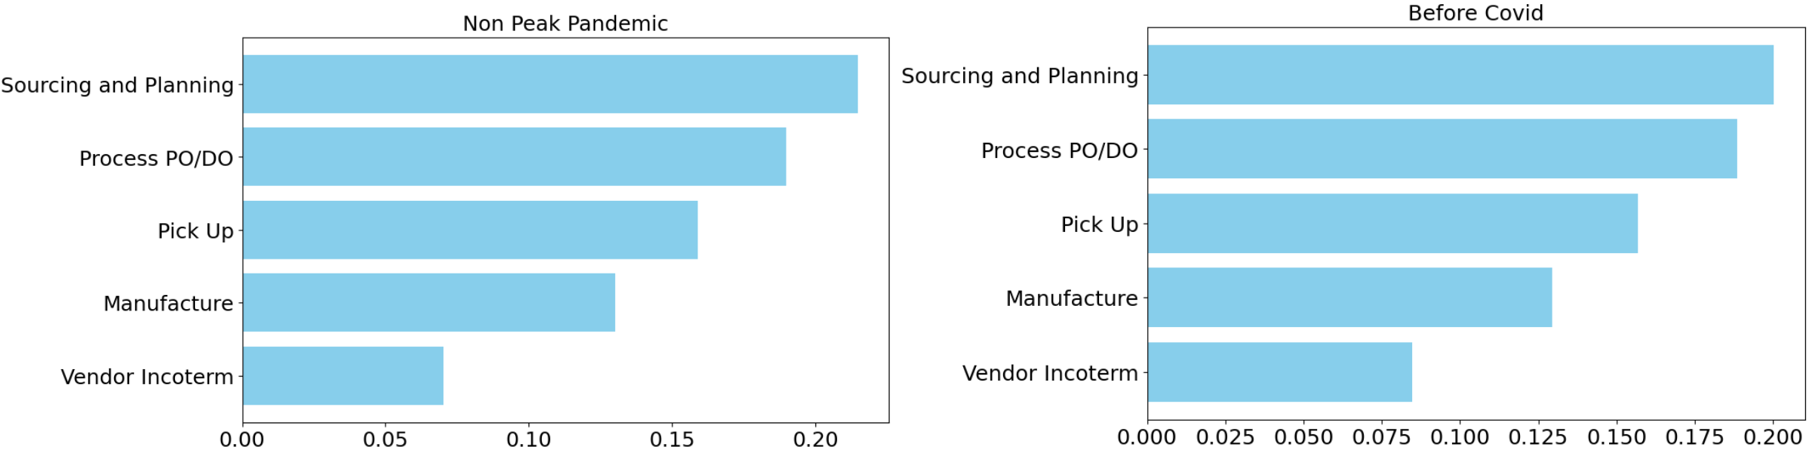
\includegraphics[width=1\textwidth]{CovidPaper/NormalOperation.png}
\caption{Top 5 features for non-peak and before pandemic}
\label{fig:normalop}
\end{figure}

\begin{figure}[ht]
\centering
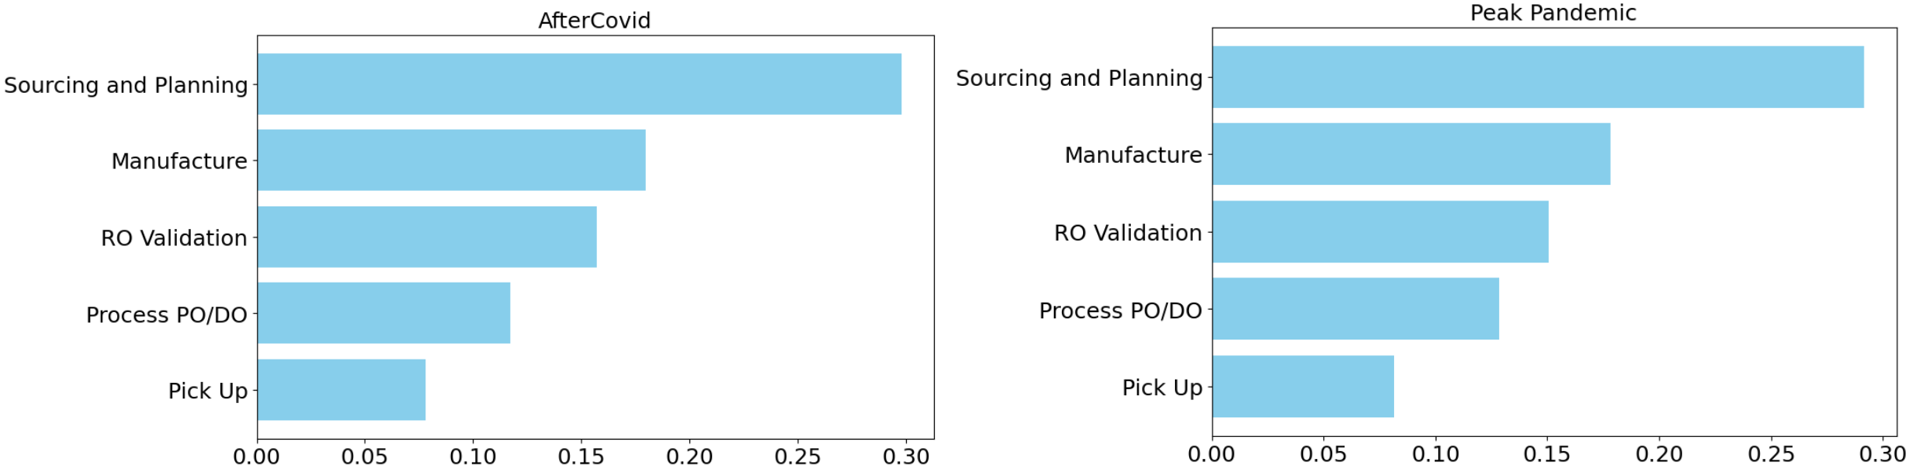
\includegraphics[width=1\textwidth]{CovidPaper/StressOperation.png}
\caption{Top 5 features for peak and after pandemic}
\label{fig:peakpandemic}
\end{figure}

Before delving into the feature analysis, it is crucial to define and understand the significance of each feature involved in the model:

\begin{itemize}
    \item \textbf{Sourcing and Planning:} Total cycle time in days to plan warehouse fulfillment for Distribution Orders or to complete sourcing for Purchase Orders.
    \item \textbf{Manufacture:} Total time in days for an order to be made ready for pick-up after order release.
    \item \textbf{RO Validation:} Total cycle time in days to complete order validation.
    \item \textbf{Process PO/DO (Purchase Order/Delivery Order):} Total time in days to release an order for fulfillment following USAID approval.
    \item \textbf{Pickup:} Total time in days for an order to be picked up for shipment.
    \item \textbf{Vendor Incoterm:} Incoterms (International Commercial Terms) define the transportation responsibilities between the buyer and seller, affecting the risk and cost responsibilities from the moment the merchandise is transferred from the seller to the buyer.
\end{itemize}

In our analysis across all time segments, \textbf{Sourcing and Planning} emerges as the most critical feature. This aligns with the fundamental principles of supply chain management, where effective sourcing and planning significantly enhance operational efficiency and responsiveness.

However, an observation from the pandemic versus normal operations analysis is the shift in importance of certain features. During the pandemic, \textbf{RO Validation} ranks among the top five features, suggesting a heightened focus on order accuracy. In contrast, during normal operations, \textbf{RO Validation} is replaced by \textbf{Vendor Incoterm}, indicating a higher priority on the terms of trade and the associated risks and costs.

This shift implies that during normal operations, the terms and conditions governing the shipment and delivery of goods are critical, potentially due to the more stable and predictable environment allowing for more focus on cost-efficiency and risk management. This might also explain why operations during normal times are less predictable than during the pandemic when strict adherence to validated processes and urgent compliance takes precedence over trade terms.

\subsection{Practical Implications}
The conventional just-in-time (JIT) approach to supply chain management is one of the most widely adopted strategies in business. This philosophy of precise synchronization optimizes both cost and time from the manufacturer’s perspective. In a globalized economy, everything must be perfectly in sync. However, any disruption in this chain can lead to delays, product availability issues, and price hikes on the consumer end, ultimately resulting in a poorer customer experience. A notable example is Toyota, the pioneer of JIT, which has started to incorporate more just-in-case elements to add buffers and maintain high service quality \cite{To_2023}.

Understanding the right balance between just-in-case and just-in-time elements is crucial, and predicting lead times plays a key role in achieving this balance. This is where our research contributes. Although our current predictive model may not yet be robust enough for fully automated systems, it could serve as a valuable supplementary tool for supply chain managers, providing an additional reference point for decision-makers. While this approach may not directly reduce lead times, the increased accuracy in lead time predictions can enhance coordination, minimize resource wastage, and prevent the costly consequences of delayed orders further down the supply chain.


\section{Conclusion}
From our research, we have developed a model that can somewhat accurately predict lead times, offering small insights into the operational differences between pandemic and normal conditions. Utilizing the Random Forest algorithm, our study achieved a median error of approximately 7 days in lead times. Notably, we also identified that RO validation takes precedence over Vendor Incoterm during pandemic times. While the result is far from being a reliable tool for a fully automated system, this current result is still a useful tool as it can act as an additional reference point. 

Looking ahead, we aim to refine our approach to data analysis to further reduce the Root Mean Square Error (RMSE). Additionally, we plan to explore more advanced machine learning models, particularly neural networks, to ascertain whether a higher degree of accuracy is achievable. While we initially opted against this due to the limitations in feature analysis with neural networks, advancing our model to accurately predict lead times under both normal and pandemic conditions remains a priority. Ultimately, our goal is to develop a real-time prediction tool that can significantly benefit practitioners in the field by providing reliable lead time estimates, enhancing decision-making and operational efficiency.



\chapter{Federated Learning Across Hospital Clusters}
\label{chap:fl_clusters}

\noindent\emph{This is one of the two new contribution chapters.} It builds on the
components of the preceding chapters---the blockchain/IPFS consent layer
(Chapter~\ref{chap:blockchain}), the compute-placement rule of
Chapter~\ref{chap:spark}, and the cross-institution heterogeneity
established in Chapter~\ref{chap:supplychain}---to specify a consent-gated
cross-silo federated learning system over the primary clinical task of
Section~\ref{sec:thesis}: 30-day readmission prediction on the Diabetes 130
cohort. Its purpose is not to demonstrate that such
a system can be built; recent work has already done that. Its purpose is to
\emph{measure what the patient autonomy it provides costs}, along the two axes
defined in Section~\ref{sec:thesis}: governance overhead (the systems cost) and
accuracy degradation under consent dynamics (the utility cost). The utility-cost
studies of this chapter have been \emph{executed}; their results are reported
below.

\section{Honest Framing of the Contribution}

This chapter and the next deliver a \emph{measurement}, not a leaderboard result.
We therefore state plainly what is and is not being claimed. The system under
test is a 30-day readmission classifier on the Diabetes 130 cohort; its
centralized ceiling is established below (AUROC $\approx 0.677$, inside the
published state-of-the-art band of 0.667--0.70 for this task) and is \emph{not}
the object of study. What is
under study is how that accuracy moves, and what governance costs, as patients
exercise dynamic, revocable consent. Peak accuracy is explicitly not the target:
chasing it would optimize the wrong quantity; indeed the task's low signal
ceiling is convenient, because it guarantees that measured degradation reflects
population change rather than under-fitting headroom. The deliverable is the
cost--utility frontier and the non-obvious findings it reveals.

\section{System Design: Consent-Gated Cross-Silo FL}
\label{sec:fl_design}

The system couples a federated coordinator with the two-tier on-chain consent
layer. Before each training round (or each consent-refresh interval, a swept
parameter), the coordinator resolves two things from the ledger: the set of
admitted hospital silos (the institutional tier, mostly static) and, within each
silo, the set of patients whose consent is currently active (the patient tier,
dynamic and revocable). Only consented records contribute to that round.

\begin{itemize}
  \item \textbf{Consent layer.} Two smart contracts---a silo registry and a
        patient-consent contract---extend the grant/revoke design of
        Chapter~\ref{chap:blockchain}. The chain stores only
        \texttt{\{patientID, consentStatus, content-identifier, key,
        authorizedViewers\}}; the encrypted FHIR-aligned record sits off-chain on
        IPFS. No clinical data is ever written to the ledger.
  \item \textbf{Training layer.} Each silo trains the readmission classifier
        locally; the coordinator aggregates with class-weighted \textbf{FedAvg}.
        FedAvg is chosen as a
        neutral baseline precisely because its sensitivity to non-IID data makes
        consent churn \emph{visible} as a utility cost---and, as the executed
        comparison below shows, because no alternative aggregator improves on it
        at this federation size.
  \item \textbf{Data.} The Diabetes 130 cohort (101{,}766 encounters;
        171 features after preprocessing; 11.2\% positive) is
        partitioned across $K{=}3$ silos with controlled non-IID skew via a
        Dirichlet$(\alpha)$ label-distribution split, from IID
        ($\alpha{\to}\infty$) to severe heterogeneity ($\alpha{=}0.1$). Synthea
        supplies the hospital-scale population for the systems-cost axis only
        (Section~\ref{sec:cost_axis}).
\end{itemize}

\subsection{Executed Baseline: Ceiling, Floor, and Aggregation Methods}
\label{sec:executed_baseline}

The reference anchors for the utility axis have been established experimentally
(five-fold cross-validation; five seeds for federated runs).

\begin{itemize}
  \item \textbf{Centralized ceiling.} A multi-model benchmark (logistic
        regression, random forest, histogram gradient boosting, XGBoost,
        LightGBM), each with imbalance handling, tops out at AUROC
        $\approx 0.677$ (random forest / XGBoost)---inside the published
        0.667--0.70 band for this task. Model choice barely moves AUROC: the
        task's signal ceiling is genuinely low.
  \item \textbf{Federated ceiling.} Trees are not weight-averageable, so the
        federated ceiling is set by the best \emph{averageable} model: logistic
        regression at AUROC $0.666$. The $\approx 0.011$ gap between the tree
        ceiling and the averageable ceiling is the first concrete, measured cost
        of federating this task.
  \item \textbf{Aggregation methods at $K{=}3$.} All five methods (FedAvg,
        FedProx, FedAvgM, FedAdam, SCAFFOLD) are statistically indistinguishable
        at IID and moderate skew (AUROC $0.666$--$0.670$), i.e.\ the aggregation
        choice barely matters until heterogeneity is pathological. The one
        exception is diagnostic: \textbf{SCAFFOLD collapses at severe skew}
        ($\alpha{=}0.1$: AUROC $0.625$), a documented small-$K$ failure mode of
        control variates over few, small, extreme silos. Class-weighted FedAvg
        is therefore the empirically justified default instrument.
\end{itemize}

\section{The Systems-Cost Axis (RQ1)}
\label{sec:cost_axis}

Every federated round is instrumented to decompose its wall-clock and monetary
cost into \emph{compute} and \emph{governance}, where governance covers
consent-set resolution, on-chain grant/revoke transactions, and encrypted-record
retrieval. Reusing the gas-and-latency methodology of
Chapter~\ref{chap:blockchain}, we sweep consent-churn rate, consent-refresh
cadence, federation size, and chain backend (local, permissioned, public), and
report per-operation \emph{distributions} rather than means, since public-chain
latency is heavy-tailed. The objective is the H1 infeasibility threshold beyond
which per-round on-chain consent cannot keep up and must be amortized across
rounds, together with the staleness that amortization introduces.

\section{The Utility-Cost Axis: Three Churn Regimes (RQ2)}
\label{sec:utility_axis}

The central experiment drives the trainer under controlled consent dynamics and
measures the resulting accuracy degradation. Crucially, we do not treat ``churn''
as one phenomenon; we separate three regimes that the literature conflates, with
permanent withdrawal further split by \emph{who} withdraws. This study has been
executed on the primary task: consent schedules are injected into the FedAvg
round loop, churn rates are swept up to 70\%, and each condition is run over
five seeds. Table~\ref{tab:churn_results} reports the degradation at the
maximum-stress setting of each regime.

\begin{enumerate}
  \item \textbf{Transient / rotating departure.} Patients withdraw consent and
        later restore it; their contributions re-enter the population.
        \emph{Measured: near-harmless} ($-0.003$ AUROC at 70\% churn).
  \item \textbf{Permanent withdrawal.} Contributions leave for good. When
        withdrawal is \emph{random}, the population shrinks without shifting and
        the cost stays small ($-0.007$ at 70\%). When withdrawal is
        \emph{biased}---positive-outcome patients leave first---the same
        headcount costs roughly three times as much ($-0.021$), because the
        training distribution itself moves. This is the natural setting for the
        federated-unlearning extension of Chapter~\ref{chap:conclusion}.
  \item \textbf{Whole-silo departure.} An institution exits, removing an entire
        slice of the distribution at once. \emph{Measured: the dominant regime}
        ($-0.059$ when the positive-heavy silo exits under severe skew,
        $\alpha{=}0.1$---roughly six times the transient cost; only $-0.010$
        when a positive-light silo exits, confirming that the damage is
        distributional, not institutional per se).
\end{enumerate}

\begin{table}[htbp]
\centering
\caption{Executed consent-churn study on the primary readmission task:
degradation ($\Delta$AUROC vs.\ the no-churn federated baseline), class-weighted
FedAvg, $K{=}3$, five seeds.}
\label{tab:churn_results}
\begin{tabular}{lr}
\toprule
Regime (maximum-stress setting) & $\Delta$AUROC \\
\midrule
Transient (rejoin), 70\% churn                          & $-0.003$ \\
Permanent, random, 70\%                                 & $-0.007$ \\
Permanent, biased (positives leave first), 70\%         & $-0.021$ \\
Whole-silo exit, positive-light silo ($\alpha{=}0.1$)   & $-0.010$ \\
Whole-silo exit, positive-heavy silo ($\alpha{=}0.1$)   & $-0.059$ \\
\emph{Count-matched random control} (same $N$ as silo exit) & $-0.039$ \\
\bottomrule
\end{tabular}
\end{table}

The headline finding is the isolation test in the last two rows: removing an
entire positive-heavy silo costs $-0.059$ AUROC, while removing the \emph{same
number of patients} drawn uniformly at random costs $-0.039$. Identity, not
headcount, carries the damage: \textbf{\emph{who} leaves matters more than
\emph{how many} leave}, confirming H2 and overturning the intuitive headcount
model of consent cost. Two honest qualifications frame this result. First,
random per-patient churn is genuinely \emph{cheap} on this task---a real, if
undramatic, finding in itself; the large costs come exclusively from
\emph{distribution shift} (biased withdrawal, silo exit). Second, the absolute
magnitudes are moderated by the large cohort, the linear averageable client, and
the rank-robustness of AUROC; a planned higher-capacity averageable client
(a small MLP) tests whether they are a linear-model artifact.

\section{Multi-Project Consent (RQ4)}
\label{sec:multiproject}

To show the framework generalizes beyond a single disease model without building a
second one, the consent layer is extended to a patient\,$\times$\,study matrix: a
patient may be enrolled in, and independently withdraw from, several federated
studies at once. Additional ``studies'' are instantiated as parameterized
federated runs over the same infrastructure rather than as new clinical models. We
measure the marginal governance cost per added study, testing H4's prediction of
bounded, sub-linear overhead because consent state is shared infrastructure.

\section{Extensibility Beyond the Clinical Model}
\label{sec:extensibility}

The consent-gated architecture is domain-agnostic. The supply-chain forecasting of
Chapter~\ref{chap:supplychain} is one candidate second tenant of the
multi-project consent layer---a federated demand model over a hospital consortium
would reuse the same governance path---but it is noted here only as evidence of
generality, not pursued as a co-equal modeling contribution within this
dissertation.


\chapter{System Integration and Evaluation}
\label{chap:integration_eval}

\noindent\emph{This is the second new contribution chapter.} It presents the
end-to-end consent-gated prototype and the experiments that produce this
dissertation's central artifact: the \emph{cost--utility frontier} of patient
autonomy. Where Chapter~\ref{chap:fl_clusters} specifies the design and the two
measurement axes, this chapter reports the integrated system and the results of
sweeping consent dynamics across it.

\section{Prototype Architecture}
\label{sec:architecture}

The prototype implements the single clinical workflow of the consent-gated
readmission model; it does not maintain a separate supply-chain pipeline (the
supply-chain domain serves as motivating evidence in
Chapter~\ref{chap:supplychain}, not as a deliverable system).

\begin{itemize}
    \item \textbf{Patient consent and data governance.} Each patient carries a
    key pair and a consent record on the
    Ethereum/IPFS consent layer of Chapter~\ref{chap:blockchain}: the chain holds
    the permission, content identifier, and key; the encrypted FHIR-aligned record
    sits off-chain on IPFS. Grant and revoke are first-class, auditable
    operations. Diabetes 130 encounters populate the silos for the utility
    studies; Synthea-generated FHIR profiles scale the population for the
    systems-cost stress tests.
    \item \textbf{Consent-resolved local processing.} At each silo, the local
    pipeline queries the consent layer before a round to obtain the currently
    consenting patient set and selects only those records for training. (Spark is
    retained at the per-silo layer for the later image-scale extension; for the
    tabular Year-1 study it is not on the critical path, consistent with the
    finding of Chapter~\ref{chap:spark}.)
    \item \textbf{Federated training.} Consented updates are aggregated with
    FedAvg; the global model returns to each silo. Every round is instrumented to
    separate compute cost from governance cost (Section~\ref{sec:cost_axis}).
\end{itemize}

\subsection{Implementation Status}
The utility-axis instrumentation is \emph{built and executed}: a modular
centralized benchmark, a churn-aware federated trainer implementing all five
aggregation methods, and a library of consent-churn schedules (transient,
permanent-random, permanent-biased, whole-silo, and the count-matched control),
with the five-seed results reported in
Sections~\ref{sec:executed_baseline}--\ref{sec:utility_axis}. A simulated
multi-silo deployment runs on a single host, with a two-machine LAN deployment
having validated the networking, serialization, and aggregation path. The next
build step is the on-chain cost instrumentation (local, permissioned, and public
backends) wired onto the existing per-round hook, with the already-built churn
schedules serving as the transaction-traffic generator---the coupling that lets
a single churn parameter drive both axes of the frontier simultaneously.

\section{Experimental Protocol}
\label{sec:protocol}
The evaluation runs the two measurement studies of
Chapter~\ref{chap:fl_clusters} end to end:
\begin{enumerate}
  \item \textbf{Systems cost (RQ1).} Per-round, per-operation latency and gas on
  local vs.\ permissioned vs.\ public chains, swept over churn rate, refresh
  cadence, and federation size; round time decomposed into compute vs.\
  governance; reported as distributions.
  \item \textbf{Utility cost (RQ2).} Accuracy, F1, ROC-AUC, PR-AUC, and
  calibration (expected calibration error) of the federated readmission model
  under each of the
  three churn regimes at each churn rate, against centralized and no-churn
  baselines, with McNemar tests for significance. \emph{Executed: see
  Section~\ref{sec:utility_axis}.}
  \item \textbf{Frontier and multi-project (RQ3, RQ4).} The joint cost--utility
  frontier with its operating ``knee,'' and the marginal governance cost per
  added study in the patient\,$\times$\,study consent matrix.
\end{enumerate}

\section{Results}
\label{sec:results}
The utility-axis results (RQ2) are in hand and reported in
Chapter~\ref{chap:fl_clusters}: the reference anchors
(Section~\ref{sec:executed_baseline}) and the three-regime degradation study
with its count-matched isolation test confirming H2
(Table~\ref{tab:churn_results}). \emph{[Remaining results to be completed as
experiments conclude.]} The central remaining result is the
cost--utility frontier (Figure to be added): model utility versus per-round
governance cost, one curve per churn regime and chain backend, with the H1
infeasibility threshold and the H3 knee annotated. Supporting tables will add
the multi-project marginal-cost
measurements (RQ4). Findings will be stated as the deltas and breaking points the
thesis targets, not as a single accuracy figure.

%%%%%%%%%%%%%%%%%%%%%%%%%%%%%%%%%%%%%%%%%%%%%%%%%%%%%%%%%%%%%%%%%%%%%%%%%%%%
% Chapter — Discussion, Conclusions, and Future Work
%%%%%%%%%%%%%%%%%%%%%%%%%%%%%%%%%%%%%%%%%%%%%%%%%%%%%%%%%%%%%%%%%%%%%%%%%%%%
\chapter{Discussion, Conclusions, and Future Work}
\label{chap:conclusion}

\section{Summary of Contributions}
This dissertation reframes patient-consent governance in cross-silo federated
learning from a feature to be built into a cost to be measured. Building on three
published components---a scalable cervical classifier
(Chapter~\ref{chap:spark}), a patient-controlled blockchain/IPFS consent layer
with a validated on-chain cost methodology (Chapter~\ref{chap:blockchain}), and a
multi-institutional regime-shift study (Chapter~\ref{chap:supplychain})---it builds
a consent-gated cross-silo FL system and measures the two-axis cost of patient
autonomy: governance overhead and utility degradation under dynamic, revocable
consent (Chapters~\ref{chap:fl_clusters}--\ref{chap:integration_eval}). Its primary
artifacts are the cost--utility frontier, the three-regime characterization of
consent churn, and the multi-project consent matrix.

\section{Limitations}
The federation is simulated rather than a live multi-hospital deployment, and
its silos are Dirichlet partitions of one cohort rather than real hospital
boundaries (real-silo replication, e.g.\ on eICU, is future work). The measured
utility magnitudes are moderated by the large cohort, the linear averageable
client, and AUROC's rank-robustness---the planned MLP client tests whether they
are a model-capacity artifact. Synthetic data is confined to the systems axis,
where signal quality is irrelevant by construction. Finally, the Year-1 system
claims consent
governance and data autonomy, not formal privacy, since FedAvg alone provides
leaky data-locality rather than a differential-privacy guarantee.

\section{Future Work}
Four extensions deepen the frontier without changing the thesis. (1)
\textbf{Privacy that earns the word:} compose differential privacy (DP-SGD) and/or
secure aggregation onto the federated trainer and measure the
noise\,$\rightarrow$\,accuracy cost as a third axis. (2) \textbf{Robustness:}
the aggregator dimension is already closed---five methods were compared and
class-weighted FedAvg justified empirically
(Section~\ref{sec:executed_baseline})---so the remaining robustness check is
model capacity: re-run the churn study with a small MLP client to test whether
the modest magnitudes are a linear-model artifact, and replicate on real
hospital silos (eICU). (3) \textbf{Federated unlearning:} on permanent withdrawal,
trigger unlearning of the revoked contribution and measure its cost---an open
problem in the consent-gating literature. (4) \textbf{Image scale:} extend to
cervical images (SipakMed), where the heavy Spark/CNN pipeline of
Chapter~\ref{chap:spark} is justified, and re-run the cost--utility study at image
scale. These constitute the multi-year arc of which this dissertation is the
foundation.

\printbibliography % Prints the bibliography using biblatex
\end{document}



